\documentclass[11pt]{book}
\oddsidemargin 0in
\evensidemargin 0in
\marginparwidth 0in
\textheight 8in
\textwidth 6.5in
\topmargin 0in
\headheight 14pt
\usepackage{amssymb,amsmath,amsthm,fancyhdr,supertabular,longtable,hhline,mathtools}
\usepackage{colortbl}
\usepackage{import, multicol,boxedminipage}
\usepackage{chapterfolder}
\usepackage[metapost,truebbox]{mfpic}
\usepackage[pdflatex]{graphicx}
\usepackage{makeidx}
\usepackage[colorlinks, hyperindex, plainpages=false, linkcolor=blue, urlcolor=blue, pdfpagelabels]{hyperref}
\usepackage[all]{hypcap}
\definecolor{ResultColor}{gray}{0.9}
\theoremstyle{definition}  % this prevents the text in definitions, theorems, and corollaries from being italicized
\newtheorem{defn}{\bf Definition}[chapter]
\newtheorem{thm}{\bf Theorem}[chapter]
\newtheorem{cor}[thm]{\bf Corollary}
\newtheorem{eqn}{\bf Equation}[chapter]
\newtheorem{ex}{\bf Example}[section]
\newtheorem{fig}{\bf Figure}[chapter]
\setlength{\parindent}{0in}
\newcommand{\bbm}{\begin{boxedminipage}{6.41in}}
\newcommand{\ebm}{\end{boxedminipage}}
\usepackage{array}
\setlength{\extrarowheight}{2pt}
\allowdisplaybreaks[2]
\usepackage{cancel}
\usepackage{sectsty}
%\usepackage{appendix}
\usepackage{textcomp}
\usepackage{multirow}
\usepackage[nottoc]{tocbibind}

\DeclareSymbolFont{AMSb}{U}{msb}{m}{n}
\DeclareMathSymbol{\C}{\mathbin}{AMSb}{"43}
\DeclareMathSymbol{\N}{\mathbin}{AMSb}{"4E}
\DeclareMathSymbol{\I}{\mathbin}{AMSb}{"5A}
\DeclareMathSymbol{\Q}{\mathbin}{AMSb}{"51}
\DeclareMathSymbol{\R}{\mathbin}{AMSb}{"52}
\DeclareMathSymbol{\W}{\mathbin}{AMSb}{"57}

\allsectionsfont{\mdseries \scshape}
\makeatletter
\renewcommand\l@section{\@dottedtocline{1}{1.5em}{3em}}
\renewcommand\l@subsection{\@dottedtocline{2}{4.5em}{3.5em}}
\newcommand{\ds}{\displaystyle}
\makeatother
\pagestyle{fancy}
\newcounter{HW}
\newcounter{HWindent}

\renewcommand{\textinterrobang}{$! \! \! ?$}

%Below is for Iowna Font
%\renewcommand*\sfdefault{iwona}
%\usepackage[math]{iwona}

%Below is for Helvetica (scaled): 
\usepackage[scaled=.92]{helvet}   
\renewcommand{\familydefault}{\sfdefault}  %makes the text of the book sans serif
\usepackage[helvet]{sfmath}  %makes the math in the book sans serif
\allsectionsfont{\sffamily}  %makes the chapter and section titles sans serif

\makeatletter
\newcases{mycases}{\quad}{%
  \hfil$\m@th\displaystyle{##}$}{$\m@th\displaystyle{##}$\hfil}{\lbrace}{.}
\makeatother

\begin{document}

\renewcommand{\textinterrobang}{$! \! \! ?$}

\chapter{\sc Sequences and the Binomial Theorem}

\section{Sequences}

\documentclass{ximera}

\begin{document}
	\author{Stitz-Zeager}
	\xmtitle{TITLE}


\mfpicnumber{1}

\opengraphsfile{Sequences}

\setcounter{footnote}{0}

\label{Sequences}

In this section, we introduce \textit{sequences} which are an important class of functions whose domains are, more or less,  the set of natural numbers.\footnote{Recall that this is the set $\mathbb{N} = \{1, 2, 3, \ldots\}$.}  Before we get to far ahead of ourselves, let's look at what the term `sequence' means mathematically.  Informally, we can think of a sequence as an infinite list of numbers.  For example, consider the sequence

 \begin{equation} \label{seq1} \frac{1}{2}, -\frac{3}{4}, \frac{9}{8}, -\frac{27}{16}, \ldots \tag{1} \end{equation} 

As usual, the periods of \index{ellipsis (\ldots)} ellipsis, $\ldots$, indicate that the proposed pattern continues forever.  Each of the numbers in the list is called a  \textit{term}, and we call $\frac{1}{2}$ the `first term', $-\frac{3}{4}$  the `second term', $\frac{9}{8}$  the `third term' and so forth.  In numbering them this way, we are setting up a function, which we'll call `$a$' per tradition, between the natural numbers and the terms in the sequence.

\setlength{\extrarowheight}{2pt}

\[ \begin{array}{|r||r|}  \hline

n & a(n)  \\[2pt]  \hline
1  & \frac{1}{2} \\[3pt]  \hline 
2 & -\frac{3}{4}  \\[3pt] \hline 
3 & \frac{9}{8}  \\[3pt] \hline 
4 & -\frac{27}{16}  \\[3pt] \hline 
\vdots & \vdots  \\[2pt] \hline
\end{array} \] 

\setlength{\extrarowheight}{0pt}

In other words, $a(n)$ is the $n^{\text{th}}$ term in the sequence.  We formalize these ideas in our definition of a  sequence and introduce some accompanying notation.

\smallskip

\colorbox{ResultColor}{\bbm

\begin{defn} \label{sequencedefn} \index{sequence ! definition of}  A \textbf{sequence} is a function $a$ whose domain is the natural numbers. The value $a(n)$ is often written as $a_{n}$ and is called the \index{sequence ! $n^{\textrm{th}}$ term}  \textbf{\boldmath $n^{\textbf{th}}$ term} of the sequence.  The sequence itself is usually denoted using the notation:  $a_{n}$, $n \geq 1$ or the notation:  $\left\{ a_{n} \right\}_{n = 1}^{\infty}$.


\end{defn}

\ebm}

\smallskip

Applying the notation provided in Definition \ref{sequencedefn} to the sequence given (\ref{seq1}), we have $a_{\text{\tiny$1$}} =  \frac{1}{2}$, $a_{\text{\tiny$2$}} =  -\frac{3}{4}$, $a_{\text{\tiny$3$}} =  \frac{9}{8}$. 

Suppose we wanted to know $a_{\text{\tiny$117$}}$, that is, the $117^{\text{th}}$ term in the sequence. While the pattern of the sequence is apparent, it would benefit us greatly to have an explicit formula for $a_{n}$.  Unfortunately, there is no general algorithm that will produce a formula for every sequence, so any formulas we do  develop will come from that greatest of teachers, experience. In other words, it is time for an example.

\begin{ex} \label{seqex1}  Write the first four terms of the following sequences.

\begin{multicols}{2}
\begin{enumerate}


\item  $a_{n} = \dfrac{5^{n-1}}{3^{n}}$, $n \geq 1$

\item  $b_{k} = \dfrac{(-1)^{k}}{2k+1}$, $k \geq 0$

\setcounter{HW}{\value{enumi}}
\end{enumerate}
\end{multicols}

\begin{multicols}{2}
\begin{enumerate}
\setcounter{enumi}{\value{HW}}

\item  $\left\{ 2n - 1 \right\}_{n=1}^{\infty} \vphantom{\left\{\dfrac{1 + (-1)^{i}}{i} \right\}_{i=2}^{\infty}}$

\item  $\left\{\dfrac{1 + (-1)^{i}}{i} \right\}_{i=2}^{\infty}$

\setcounter{HW}{\value{enumi}}
\end{enumerate}
\end{multicols}

\begin{multicols}{2}
\begin{enumerate}
\setcounter{enumi}{\value{HW}}


\item\label{introrecursiveex01}  $a_{\text{\tiny$1$}} = 7$, $a_{n \text{\tiny$ + 1$}} = 2 - a_{n}$, $n \geq 1$

\item  \label{factorialintroex} $f_{\text{\tiny$0$}} = 1$, $f_{n} =n \cdot f_{n-\text{\tiny$1$}}$, $n \geq 1$

\setcounter{HW}{\value{enumi}}
\end{enumerate}
\end{multicols}



{\bf Solution.}

\begin{enumerate}

\item Since we are given $n \geq 1$, the first four terms of the sequence are  $a_{\text{\tiny$1$}}$, $a_{\text{\tiny$2$}}$, $a_{\text{\tiny$3$}}$ and $a_{\text{\tiny$4$}}$.  Since the notation $a_{\text{\tiny$1$}}$ means the same thing as $a(1)$, we obtain our first term by replacing every occurrence of $n$ in the formula for $a_{n}$ with $n=1$ to get  $a_{\text{\tiny$1$}} = \frac{5^{1-1}}{3^{1}} = \frac{1}{3}$.  Proceeding similarly, we get $a_{\text{\tiny$2$}} = \frac{5^{2-1}}{3^{2}} =\frac{5}{9}$, $a_{\text{\tiny$3$}} = \frac{5^{3-1}}{3^{3}} =\frac{25}{27}$ and $a_{\text{\tiny$4$}} = \frac{5^{4-1}}{3^{4}} =\frac{125}{81}$.  

\item For this sequence we have $k \geq 0$, so the first four terms are $b_{\text{\tiny$0$}}$, $b_{\text{\tiny$1$}}$, $b_{\text{\tiny$2$}}$ and $b_{\text{\tiny$3$}}$.  Proceeding as before, replacing in this case the variable $k$ with the appropriate whole number, beginning with $0$, we get $b_{\text{\tiny$0$}} = \frac{(-1)^{0}}{2(0)+1} = 1$, $b_{\text{\tiny$1$}} = \frac{(-1)^{1}}{2(1)+1} = - \frac{1}{3}$, $b_{\text{\tiny$2$}} = \frac{(-1)^{2}}{2(2)+1} = \frac{1}{5}$ and $b_{\text{\tiny$3$}} =  \frac{(-1)^{3}}{2(3)+1} = -\frac{1}{7}$.  As a side-note, this sequence is called an \index{sequence ! alternating} \textit{alternating} sequence since the signs alternate between `$+$' and `$-$.' The reader is encouraged to think what component of the formula is producing this effect.

\item  The notation $\left\{ 2n - 1 \right\}_{n=1}^{\infty}$ means  $a_{n} = 2n -1$, $n \geq 1$.  We get $a_{\text{\tiny$1$}} = 1$, $a_{\text{\tiny$2$}} = 3$, $a_{\text{\tiny$3$}} = 5$ and $a_{\text{\tiny$4$}} = 7$.  In other words, we get the first four odd natural numbers.  The reader is encouraged to examine whether or not this pattern continues indefinitely.

\item  Here, we are using the letter $i$ as a counter, not as the imaginary unit we saw in Section \ref{ComplexZeros}.  Proceeding as before, we set $a_{i} = \frac{1 + (-1)^{i}}{i}$, $i \geq 2$.  We find $a_{\text{\tiny$2$}} = 1$, $a_{\text{\tiny$3$}} = 0$, $a_{\text{\tiny$4$}} = \frac{1}{2}$ and $a_{\text{\tiny$5$}} = 0$.  

\item  To obtain the terms of this sequence, we start with $a_{\text{\tiny$1$}} = 7$ and use the equation $a_{n \text{+\tiny$1$}} = 2 - a_{n}$ for $n \geq 1$ to generate successive terms.  When $n = 1$, this equation becomes $a_{\text{\tiny$1 + 1$}} = 2 - a_{\text{\tiny$1$}}$ which simplifies to $a_{\text{\tiny$2$}} = 2 - a_{\text{\tiny$1$}} = 2 - 7 = -5$.  When $n = 2$, the equation becomes $a_{\text{\tiny$2 + 1$}} = 2 - a_{\text{\tiny$2$}}$ so we get $a_{\text{\tiny$3$}} = 2 - a_{\text{\tiny$2$}} = 2 - (-5) = 7$.  Finally, when $n = 3$, we get $a_{\text{\tiny$3 + 1$}} = 2 - a_{\text{\tiny$3$}}$ so $a_{\text{\tiny$4$}} = 2 - a_{\text{\tiny$3$}} = 2-7 = -5$.  

\item  As with the problem above, we are given a place to start with $f_{\text{\tiny$0$}} = 1$ and given a formula to build other terms of the sequence.  Substituting $n = 1$ into the equation $f_{n} = n \cdot f_{n-\text{\tiny$1$}}$, we get $f_{\text{\tiny$1$}} = 1 \cdot f_{\text{\tiny$0$}} = 1 \cdot 1 = 1$.  Advancing to $n = 2$, we get $f_{\text{\tiny$2$}} = 2 \cdot f_{\text{\tiny$1$}} = 2 \cdot 1 = 2$.  Finally, $f_{\text{\tiny$3$}} = 3 \cdot f_{\text{\tiny$2$}} = 3 \cdot 2 = 6$.  \qed

\end{enumerate}

\end{ex}

Some remarks about Example \ref{seqex1} are in order. We first note that since sequences are functions, we can graph them in the same way we graph functions.  For example, if we wish to graph the sequence $\left\{ b_{k} \right\}_{k=0}^{\infty}$ from Example \ref{seqex1}, we graph the equation $y=b(k)$ for the values $k \geq 0$. That is, we plot the points $(k, b(k))$ for the values of $k$ in the domain, $k = 0, 1, 2, \ldots$.  The resulting collection of points is the graph of the sequence.  Note that we do not connect the dots in a pleasing fashion as we are used to doing, because the domain is just the whole numbers in this case, not a collection of intervals of real numbers.\footnote{If you feel a sense of nostalgia, you should see Section \ref{FunctionsandtheirRepresentations}.}
\begin{center}

\begin{mfpic}[20]{-1}{4}{-2}{2}
\point[4pt]{(0,1), (1,-0.3333), (2,0.2), (3, -0.1428) }
\axes
\tlabel[cc](4,-0.5){\scriptsize $k$}
\tlabel[cc](0.5,2){\scriptsize $y$}
\xmarks{1,2,3}
\ymarks{-1.5, -1, -0.5, 0.5, 1, 1.5}
\tlpointsep{10pt}
\axislabels {x}{{\tiny $1$} 1, {\tiny $2$} 2, {\tiny $3$} 3}
\tlpointsep{4pt}
\axislabels {y}{{\tiny $-\frac{3}{2}$} -1.5, {\tiny $-1$} -1, {\tiny $-\frac{1}{2}$} -0.5, {\tiny $\frac{1}{2}$} 0.5, {\tiny $1$} 1, {\tiny $\frac{3}{2}$} 1.5}
\end{mfpic}

Graphing  $y = b_{k} = \dfrac{(-1)^{k}}{2k+1}$, $k \geq 0$

\end{center}

Speaking of $\left\{ b_{k} \right\}_{k=0}^{\infty}$, the astute and mathematically minded reader will correctly note that this technically isn't a sequence, since according to Definition \ref{sequencedefn}, sequences are functions whose domains are the \textit{natural} numbers, not the \textit{whole} numbers, as is the case with $\left\{ b_{k} \right\}_{k=0}^{\infty}$.  In other words, to satisfy Definition \ref{sequencedefn}, we need to shift the variable $k$ so it starts at $k=1$ instead of $k=0$.  

To see how we can do this, it helps to think of the problem graphically.  What we want is to shift the graph of $y=b(k)$ to the right one unit, and thinking back to Section \ref{Transformations}, we can accomplish this by replacing $k$ with $k-1$ in the definition of $\left\{ b_{k} \right\}_{k=0}^{\infty}$.  

Specifically, let $c_{k} = b_{k-\text{\tiny$1$}}$ where $k - 1 \geq 0$.  We get $c_{k} = \frac{(-1)^{k-1}}{2(k-1)+1} = \frac{(-1)^{k-1}}{2k-1}$, where now $k \geq 1$. We leave to the reader to verify that $\left\{ c_{k} \right\}_{k=1}^{\infty}$ generates the same list of numbers as does $\left\{ b_{k} \right\}_{k=0}^{\infty}$, but the former satisfies Definition \ref{sequencedefn}, while the latter does not.   

Like so many things in this text, we acknowledge that this point is pedantic and join the vast majority of authors who adopt a more relaxed view of Definition \ref{sequencedefn} to include any function which generates a list of numbers which can then be matched up with the natural numbers.\footnote{We're basically talking about the `countably infinite' subsets of the real number line when we do this.}   


 One last note about Example \ref{seqex1} concerns the manner in which the sequences in numbers  \ref {introrecursiveex01} and \ref{factorialintroex} are defined.  We say these two sequences are  described \index{sequence ! recursive} `\textit{recursively}.'  In each instance, an initial value of the sequence is given which is then followed by a \index{recursion equation} \textit{recursion equation} $-$ a formula which enables us to use known terms of the sequence to determine other terms.  
 
 The terms of the sequence from number  \ref{factorialintroex} is given notation and name:  $f_{n}=n!$ is called \index{factorial} \textit{$n$-factorial}.  Using the `!' notation, we can describe the factorial sequence as: $0! = 1$ and $n! = n(n-1)!$ for $n \geq 1$. 
 
 After $0! = 1$ the next four terms, written out in detail, are $1! = 1 \cdot 0! = 1 \cdot 1 = 1$, $2! = 2 \cdot 1! = 2 \cdot 1 = 2$, $3! = 3 \cdot 2! = 3 \cdot 2 \cdot 1 = 6$ and  $4! = 4 \cdot 3! = 4 \cdot 3 \cdot 2 \cdot 1 = 24$.  From this, we see a more informal way of computing  $n!$, which is $n! = n\cdot(n -1)\cdot(n -2) \cdots 2 \cdot 1$ with $0! = 1$ as a special case.  (We will study factorials in greater detail in Section \ref{Binomial}.)\footnote{Another  famous sequence, the \href{http://en.wikipedia.org/wiki/Fibonacci_number}{\underline{Fibonacci Numbers}} are defined also recursively and are explored in the exercises.}  
 
 While none of the sequences in Example \ref{seqex1} worked out to be the sequence in (\ref{seq1}), they do give us some insight into what kinds of patterns to look for.  Two patterns in particular are given in the next definition.

\smallskip

\colorbox{ResultColor}{\bbm
\begin{defn}  \label{arithgeodefn}  \textbf{Arithmetic and Geometric Sequences:}  Suppose $\left\{ a_{n} \right\}_{n=k}^{\infty}$ is a sequence\footnote{Note that we have adjusted for the fact that not all `sequences' begin at $n=1$.}

\begin{itemize}

\item If  there is a number $d$ so that $a_{n \text{\tiny$ + 1$}}  = a_{n} + d$ for all $n \geq k$, then $\left\{ a_{n} \right\}_{n=k}^{\infty}$ is called an \index{sequence ! arithmetic ! definition of}\index{arithmetic sequence}\textbf{arithmetic sequence}.  The number $d$ is called the \index{sequence ! arithmetic ! common difference} \textbf{common difference}.

\item If  there is a number $r$ so that $a_{n \text{\tiny$ + 1$}} = r a_{n}$ for all $n \geq k$, then $\left\{ a_{n} \right\}_{n=k}^{\infty}$ is called a \index{sequence ! geometric ! definition of}\index{geometric sequence}\textbf{geometric sequence}.  The number $r$ is called the \index{sequence ! geometric ! common ratio}\textbf{common ratio}.

\end{itemize}


\end{defn}
\ebm}

\smallskip  

In English, an arithmetic sequence is one in which we proceed from one term to the next by always \textit{adding} the fixed number $d$.  If this sort of `constant change' idea sounds familiar, it should.  Indeed, arithmetic sequences are merely \textit{linear} functions, something we will explore in more detail shortly.  Note the name `common difference' comes from a slight rewrite of the recursion equation from $a_{n \text{\tiny$ + 1$}}  = a_{n} + d$ to $a_{n \text{\tiny$ + 1$}} - a_{n} = d$.  That is, every pair of successive terms has the \textit{same} or \textit{common} difference,  $d$.

Analogously, a geometric sequence is one in which we proceed from one term to the next by always \textit{multiplying} by the same fixed number $r$. If this notion sounds familiar, it is because geometric sequences are, in fact, \textit{exponential} functions.  Again, we will explore this connection in more detail later.  We note that if $a_{n} \neq 0$, we can rearrange the recursion equation to get $\frac{a_{n+1}}{a_{n}} = r$.  Hence, every pair of successive terms has the \textit{same} or \textit{common} ratio, $r$.  


Some sequences are arithmetic, some are geometric and some are neither as the next example illustrates.\footnote{Can a sequence be both arithmetic \textit{and} geometric?  See Exercise \ref{arithmeticandgeometricexercise}.}

\begin{ex}  \label{arithgeoex1}  Determine if the following sequences are arithmetic, geometric or neither.  If arithmetic, find the common difference $d$; if geometric, find the common ratio $r$.

\begin{multicols}{2}
\begin{enumerate}


\item  $a_{n} = \dfrac{5^{n-1}}{3^{n}}$, $n \geq 1$

\item  $b_{k} = \dfrac{(-1)^{k}}{2k+1}$, $k \geq 0$

\setcounter{HW}{\value{enumi}}
\end{enumerate}
\end{multicols}

\begin{multicols}{2}
\begin{enumerate}
\setcounter{enumi}{\value{HW}}


\item  $\left\{ 2n - 1 \right\}_{n=1}^{\infty} \vphantom{\dfrac{1}{2}, -\dfrac{3}{4}, \dfrac{9}{8}, -\dfrac{27}{16}, \ldots}$

\item  $\dfrac{1}{2}, -\dfrac{3}{4}, \dfrac{9}{8}, -\dfrac{27}{16}, \ldots$

\setcounter{HW}{\value{enumi}}
\end{enumerate}
\end{multicols}

{\bf Solution.}  A good rule of thumb to keep in mind when working with sequences is ``When in doubt, write it out!''  Writing out the first several terms can help you identify the pattern of the sequence should one exist.

\begin{enumerate}

\item  From Example \ref{seqex1}, we know that the first four terms of this sequence are $\frac{1}{3}, \, \frac{5}{9}, \, \frac{25}{27}$ and $\frac{125}{81}$.  To see if this is an arithmetic sequence, we look at the successive differences of terms.  We find that $a_{\text{\tiny$2$}} - a_{\text{\tiny$1$}} = \frac{5}{9} - \frac{1}{3} = \frac{2}{9}$ and $a_{\text{\tiny$3$}} - a_{\text{\tiny$2$}} = \frac{25}{27} - \frac{5}{9} = \frac{10}{27}$.  Since we get different numbers, there is no `common difference' and we have established that the sequence is \textit{not} arithmetic.  

To see if the sequence is geometric, we compute the ratios of successive terms.  The first three ratios  \textit{suggest} the sequence is geometric:   \[\frac{a_{\text{\tiny$2$}}}{a_{\text{\tiny$1$}}} = \frac{\frac{5}{9}}{\frac{1}{3}} = \frac{5}{3}, \;\;\; \frac{a_{\text{\tiny$3$}}}{a_{\text{\tiny$2$}}} = \frac{\frac{25}{27}}{\frac{5}{9}} = \frac{5}{3} \;\; \text{ and } \;\; \frac{a_{\text{\tiny$4$}}}{a_{\text{\tiny$3$}}} = \frac{\frac{125}{81}}{\frac{25}{27}} = \frac{5}{3}\] 
To \textit{prove} the sequence is geometric, however, we must show that $\frac{a_{n+1}}{a_{n}} = r$ for all $n$:

\[ \dfrac{a_{n\text{\tiny$ + 1$}}}{a_{n}} = \dfrac{\dfrac{5^{(n+1)-1}}{3^{n+1}}}{\dfrac{5^{n-1}}{3^{n}}} = \dfrac{5^{n}}{3^{n+1}} \cdot \dfrac{3^{n}}{5^{n-1}} = \dfrac{5}{3} \]

Hence, the sequence is geometric with common ratio $r = \frac{5}{3}$.

\item Again, we have Example \ref{seqex1} to thank for providing the first four terms of this sequence: $1, \, -\frac{1}{3}, \, \frac{1}{5}$ and $-\frac{1}{7}$.  We find $b_{\text{\tiny$1$}} - b_{\text{\tiny$0$}} =  -\frac{4}{3}$ and $b_{\text{\tiny$2$}} - b_{\text{\tiny$1$}} = \frac{8}{15}$.  Hence, the sequence is not arithmetic.  To see if it is geometric, we compute $\frac{b_{\text{\tiny$1$}}}{b_{\text{\tiny$0$}}} = -\frac{1}{3}$ and $\frac{b_{\text{\tiny$2$}}}{b_{\text{\tiny$1$}}} = -\frac{3}{5}$.  Since there is no `common ratio,' we conclude the sequence is not geometric, either.

\item  As we saw in Example \ref{seqex1}, the sequence $\left\{ 2n - 1 \right\}_{n=1}^{\infty}$ generates the odd numbers:  $1, 3, 5, 7, \ldots$.  Computing the first few differences, we find $a_{\text{\tiny$2$}} - a_{\text{\tiny$1$}} = 2$, $a_{\text{\tiny$3$}} - a_{\text{\tiny$2$}} = 2$, and $a_{\text{\tiny$4$}} - a_{\text{\tiny$3$}} = 2$.  This suggests that the sequence is arithmetic.  To prove this is the case, we find \[a_{n \text{\tiny$ + 1$}} - a_{n} = (2(n+1)-1) - (2n-1) = 2n+2-1-2n+1 = 2\]  This establishes that the sequence is arithmetic with common difference $d = 2$.  To see if it is geometric, we compute $\frac{a_{\text{\tiny$2$}}}{a_{\text{\tiny$1$}}} = 3$ and  $\frac{a_{\text{\tiny$3$}}}{a_{\text{\tiny$2$}}} = \frac{5}{3}$.  Since these ratios are different, we conclude the sequence is not geometric.

\item  We met our last sequence at the beginning of the section.  Given that $a_{\text{\tiny$2$}} - a_{\text{\tiny$1$}} = -\frac{5}{4}$ and $a_{\text{\tiny$3$}} - a_{\text{\tiny$2$}} = \frac{15}{8}$, the sequence is not arithmetic.  Computing the first few ratios, however, gives us $\frac{a_{\text{\tiny$2$}}}{a_{\text{\tiny$1$}}} = -\frac{3}{2}$, $\frac{a_{\text{\tiny$3$}}}{a_{\text{\tiny$2$}}} = -\frac{3}{2}$ and $\frac{a_{\text{\tiny$4$}}}{a_{\text{\tiny$3$}}} = -\frac{3}{2}$.  Since these are the only terms given to us, we \textit{assume} that the pattern of ratios continue in this fashion and conclude that the sequence is geometric. \qed

\end{enumerate}

\end{ex}

We are now one step away from determining an explicit formula for the sequence given in (\ref{seq1}).  We know that it is a geometric sequence and our next result gives us the explicit formula we require.

\smallskip

\colorbox{ResultColor}{\bbm

\begin{eqn}  \label{arithgeoformula}  \textbf{Formulas for Arithmetic and Geometric Sequences:} 

\begin{itemize}

\item  \index{sequence ! arithmetic ! formula for $n^{\textrm{th}}$ term}An arithmetic sequence with first term $a_{1} = a$ and common difference $d$ is given by \[a_{n} = a + (n-1) d, \quad n \geq 1\] 

%\vspace{-.3in}

\item  \index{sequence ! geometric ! formula for $n^{\textrm{th}}$ term}A geometric sequence with first term $a_{1} = a$ and common ratio $r \neq 0$ is given by  \[ a_{n} = ar^{n-1}, \quad n \geq 1\] 

%\vspace{-.2in}

\end{itemize}

\end{eqn}

\ebm}

\smallskip


An intuitive way to arrive at Equation \ref{arithgeoformula} appeals to Definition \ref{arithgeodefn} directly.  Given an arithmetic sequence with first term $a$ and common difference $d$, the way we get from one term to the next is by adding $d$.  Hence, the terms of the sequence are:  $a$, $a+d$, $a+2d$, $a+3d$, \ldots.  We see that to reach the $n$th term, we add $d$ to $a$ exactly $(n-1)$ times, which is exactly what the formula says.\footnote{We formalize this argument in Section \ref{Induction}.}

Note if we rewrite the formula $a_{n} = a_{1} + (n-1) d$ using traditional function notation as  $a(n) = a(1) + d (n-1)$ we can see arithmetic sequences are linear functions.\footnote{Note here $a$ is a \textit{function}, so the expressions $a(n)$ and $a(1)$ here represent the \textit{outputs} from $a$.  On the other hand, the expression $d(n-1)$ indicates \textit{multiplication} of the real numbers $d$ and $(n-1)$.}  Indeed, relabeling the function $a$ as `$f$' and the independent variable $n$ as `$x$,' we can make the identifications $x_{0} = 1$, and $m=d$ so as to put the equation $a(n) = a(1) + d  (n-1)$ into the form of Equation \ref{linearfunctionpointslope}: 

\[ \begin{array}{ccccc}
a(n) & = & a(1) & + & d (n-1) \\
 f(x) & = & f(1) & + & m (x-1) \\ \end{array} \]


Hence,  arithmetic sequences are linear functions with slope $d$ whose domains are the natural numbers.


The derivation of the formula for geometric series follows similarly.  Here, we start with the first term $a$ and go from one term to the next by multiplying by $r$.  We get $a, ar, ar^2, ar^3$ and so forth.  The $n$th term results from multiplying $a$ by $r$ exactly $(n-1)$ times.\footnote{We note here that the reason $r=0$ is excluded from Equation \ref{arithgeoformula} is to avoid an instance of $0^{0}$ which is an indeterminate form. (See the remarks following Definition \ref{monomialfunction} in Section \ref{GraphsofPolynomials}.)} 

In the same way  arithmetic sequences are linear functions, geometric sequences are exponential functions.  Writing  $a_{n} = a_{1} r^{n-1}$ as $a(n) = a(1) r^{n-1}$,  we can relabel $a$ as $f$ and $n$ as $x$ and make the identifications $x_{0} = 1$ and $b = r$ to put the equation into the form described in  Definition \ref{expfcnpointbaseform}:

\[ \begin{array}{ccc}
a(n) & = & a(1) r^{n-1} \\
 f(x) & = & f(1) b^{x-1} \\ \end{array} \]

So, geometric sequences are exponential functions with base $r$ whose domains are the natural numbers.

With Equation \ref{arithgeoformula} in place, we finally have the tools required to find an explicit formula for the $n$th term of the sequence given in (\ref{seq1}). We know from Example \ref{arithgeoex1} that it is geometric with common ratio $r = -\frac{3}{2}$.  The first term is $a = \frac{1}{2}$ so by Equation \ref{arithgeoformula} we get $a_{n} = ar^{n-1} = \frac{1}{2} \left( - \frac{3}{2}\right)^{n-1}$ for $n \geq 1$.  After a touch of simplifying, we get $a_{n} = \frac{(-3)^{n-1}}{2^{n}}$ for $n \geq 1$. Note that we can easily check our answer by substituting in values of $n$ and seeing that the formula generates the sequence given in (\ref{seq1}).  We leave this to the reader.  In particular, the 117th term in the sequence is $a_{117} = \frac{1}{2} \left(-\frac{3}{2} \right)^{117-1} = \frac{3^{116}}{2^{117}}$.

Our next example gives us more practice finding patterns.



\begin{ex}  \label{seqex2}  Find an explicit formula for the $n^{\text{\scriptsize th}}$ term of the following sequences.

\begin{multicols}{3}
\begin{enumerate}

\item  $0.9, 0.09, 0.009, 0.0009, \ldots$

\item  $\dfrac{2}{5}, 2, -\dfrac{2}{3}, -\dfrac{2}{7}, \ldots$

\item  $1, -\dfrac{2}{7}, \dfrac{4}{13}, -\dfrac{8}{19}, \ldots$

\end{enumerate}
\end{multicols}

{\bf Solution.}

\begin{enumerate}



\item  Although this sequence may seem strange, the reader can verify it is actually a geometric sequence with common ratio $r = 0.1 = \frac{1}{10}$. With $a = 0.9 = \frac{9}{10}$, we get $a_{n} = \frac{9}{10} \left(\frac{1}{10}\right)^{n-1}$ for $n \geq 0$.  Simplifying, we get $a_{n} = \frac{9}{10^{n}}$, $n \geq 1$.  There is more to this sequence than meets the eye and we shall return to this example in the next section.
 

\item As the reader can verify, this sequence is neither arithmetic nor geometric.  In an attempt to find a pattern, we rewrite the second term with a denominator to make all the terms appear as fractions and associate the `$-$' with the denominators so we have a constant numerator:  

\[ \frac{2}{5}, \frac{2}{1}, \frac{2}{-3}, -\frac{2}{-7}, \ldots \]

 This tells us that we can tentatively sketch out the formula for the sequence as $a_{n} = \frac{2}{D_{n}}$ where $D_{n}$ is the sequence of denominators.  
 
The sequence of the denominators: $5,1,-3,-7, \ldots$ is seen to be an arithmetic sequence with a common difference of $-4$.   Using Equation \ref{arithgeoformula} with $a = 5$ and $d = -4$, we get the $n$th denominator by the formula $D_{n} = 5 + (n-1)(-4) = 9-4n$ for $n \geq 1$. Hence, our final answer is $a_{n} = \frac{2}{9-4n}$, $n \geq 1$.


\item  The sequence as given is neither arithmetic nor geometric, so we proceed as in the last problem to try to get patterns individually for the numerator and denominator.  Letting $C_{n}$ and $D_{n}$ denote the sequence of numerators and denominators, respectively,  so that $a_{n} = \frac{C_{n}}{D_{n}}$. 

 After some experimentation,\footnote{Here we take `experimentation' to mean a frustrating guess-and-check session.} we choose to write the first term as a fraction and associate the negatives `$-$' with the numerators.  This yields \[ \frac{1}{1}, \frac{-2}{7}, \frac{4}{13}, \frac{-8}{19}, \ldots \] 
 
 The numerators form the sequence $1, -2, 4, -8, \ldots$ which is geometric with $a=1$ and $r = -2$, so we get $C_{n} = (-2)^{n-1}$, for $n \geq 1$.  
 
 The denominators $1, 7, 13, 19, \ldots$ form an arithmetic sequence with $a = 1$ and $d = 6$.  Hence, we get $D_{n} = 1 + 6(n-1) = 6n-5$, for $n \geq 1$.  
 
 Putting these two formulas together, we obtain our formula for $a_{n} = \frac{C_{n}}{D_{n}} = \frac{(-2)^{n-1}}{6n-5}$, for $n \geq 1$.  We leave it to the reader to show that this checks out. \qed

\end{enumerate}

\end{ex}

While the last problem in Example \ref{seqex2} was neither geometric nor arithmetic, it did resolve into a combination of these two kinds of sequences.  If handed the sequence $2, 5, 10, 17, \ldots$, we would be hard-pressed to find a formula for $a_{n}$ if we restrict our attention to these two archetypes.  We said before that there is no general algorithm for finding the explicit formula for the $n$th term of a given sequence, and it is only through experience gained from evaluating sequences from explicit formulas that we learn to begin to recognize number patterns.  

The pattern $1, 4, 9, 16, \ldots$ is rather recognizable as the squares, so the formula $a_{n} = n^2$, $n \geq 1$ may not be too hard to determine.  With this in mind, it's possible to see  $2, 5, 10, 17, \ldots$ as the sequence $1 + 1, 4 + 1, 9 + 1, 16 + 1 , \ldots$, so that $a_{n} = n^2 + 1$, $n \geq 1$.  

Of course, since we are given only a small \textit{sample} of the sequence, we shouldn't be too disappointed to find out this isn't the \textit{only} formula which generates this sequence.  For example, consider the sequence defined by $b_{n} = -\frac{1}{4} n^4 + \frac{5}{2} n^3 - \frac{31}{4} n^2 + \frac{25}{2} n - 5$, $n \geq 1$.  The reader is encouraged to verify that it also produces the  terms  $2, 5, 10, 17$.  In fact, it can be shown that given any finite sample of a sequence, there are infinitely many explicit formulas all of which generate those same finite points.  This means that there will be infinitely many correct answers to some of the exercises in this section.\footnote{For more on this, see \href{http://www.math.kent.edu/~white/papers/pattern.pdf}{\underline{When Every Answer is Correct: Why
Sequences and Number Patterns Fail the Test}}.}  Just because your answer doesn't match ours doesn't mean it's wrong.  As always, when in doubt, write your answer out.  As long as it produces the same terms in the same order as what the problem wants, your answer is correct.  

\smallskip

Sequences play a major role in the Mathematics of Finance, as we have already seen with Equation \ref{compoundinterest} in Section \ref{ExpLogApplications}.  Recall that if we invest $P$ dollars at an annual percentage rate $r$ and compound the interest $n$ times per year,  the formula for $A_{k}$, the amount in the account after $k$ compounding periods, is $A_{k} = P\left(1 + \frac{r}{n}\right)^{k} = \left[P\left(1 + \frac{r}{n}\right)\right]\left(1 + \frac{r}{n}\right)^{k-1}$, $ k \geq 1$.  We leave it to the reader to show this is a geometric sequence with first term $P\left(1 + \frac{r}{n}\right)$ and common ratio $\left(1 + \frac{r}{n}\right)$. 

\medskip

 In section \ref{ExpLogApplications}, we showed $\ds{\lim_{n \rightarrow \infty} P\left(1 + \frac{r}{n}\right)^{nt} = Pe^{rt}}$, where we noted, at the time, that the limit here was taken on a discrete, rather than continuous variable.  That didn't stop us from using the limit properties listed in Theorem \ref{LimitProp01}.  We talk more on the limits of sequences next.


\subsection{Limits of Sequences}
\label{sequencelimits}



Consider the sequence $a_{n} = \frac{3n}{n+1}$, $n \geq 1$. Suppose we wished to find $\ds{\lim_{n \rightarrow \infty} a_{n}}$.

\medskip

We should first note that even though the domain of the sequence $a_{n}$ is discrete, we can nonetheless discuss what happens as $n \rightarrow \infty$ since for any real number $M>0$, we can find a natural number $n > M$.  (We could, for instance take $n  = \lfloor M \rfloor + 1$.)  

\medskip

Next, note that we can visualize  the sequence $a_{n} = \frac{3n}{n+1}$, $n \geq 1$ as being points on the graph of $f(x) = \frac{3x}{x+1}$:

\begin{center}

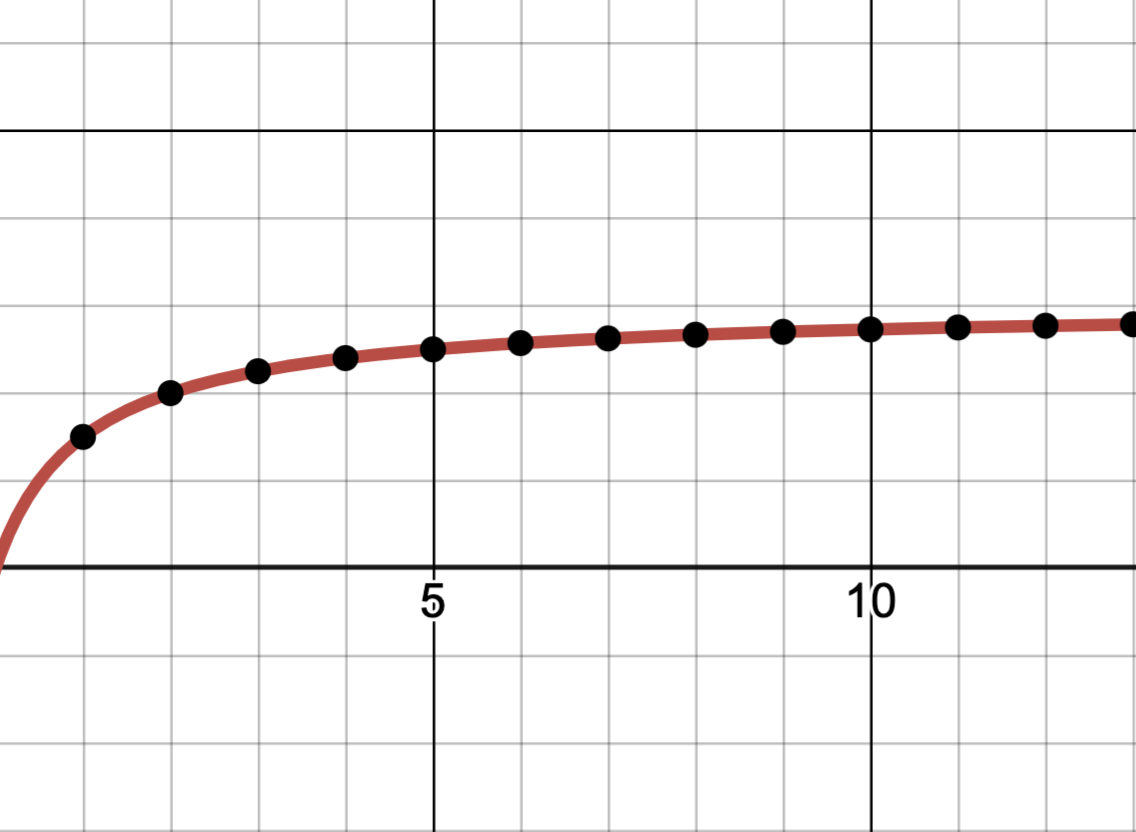
\includegraphics[width=3in]{./SequenceGraphics/sequenceoncurve.png}

\end{center}

Comparing leading terms of numerator and denominator, as $x \rightarrow \infty$, $\frac{3x}{x+1} \approx \frac{3x}{x} = 3$.   Hence,  $\ds{\lim_{x \rightarrow \infty}}$ $\frac{3x}{x+1} = 3$, which means \textbf{all} of the $y$-values on the graph of $y = f(x)$, including the $y$-values of the graph of the sequence,  approach $3$ as $x \rightarrow \infty$.  It stands to reason, then that $\ds{\lim_{n \rightarrow \infty}}$  $\frac{3n}{n+1} = 3$.


\medskip

The long and short of the above argument is that since $\ds{\lim_{x\rightarrow \infty}}$ $\frac{3x}{x+1}$ exists, $\ds{\lim_{n \rightarrow \infty}}$   $\frac{3n}{n+1} = $ $\ds{\lim_{x \rightarrow \infty}}$ $\frac{3x}{x+1}$.  While the syntax of `$\ds{\lim_{n \rightarrow \infty}}$  $\frac{3n}{n+1} =$ $\ds{\lim_{x \rightarrow \infty}}$  $\frac{3x}{x+1}$' appears to be just a switch in a dummy variable,\footnote{which it would be without context}  the switch from `$n$' to `$x$' indicates switching from a \textbf{discrete} variable to a \textbf{continuous} one. This sort of maneuver is called \index{continuous variable ! passing to}\index{passing to a continuous variable}\textbf{passing to a continuous variable} and is one of the primary ways we can use what we've already studied to analyze limits of sequences.  

\medskip

\colorbox{ResultColor}{\bbm

\begin{thm}\label{passingtocontinuous}   If $\ds{ \lim_{x \rightarrow \infty} f(x) = L}$  and $f(n) = a_{n}$  for all $n \geq k$ for some natural number $k$, then $\ds{ \lim_{n \rightarrow \infty} a_{n} = L}$.

\end{thm}

\ebm}

\medskip

Note the phrase `$f(n) = a_{n}$  for all $n \geq k$ for some natural number $k$' indicates the focus on what is happening as $n \rightarrow \infty$. In other words, the first finitely many sequence values do not impact the value of $\ds{\lim_{n \rightarrow \infty} a_{n}}$.  We are just concerned with the long-run or end behavior here.  The reason Theorem \ref{passingtocontinuous}  works, indeed why all of the limit properties discussed in Section \ref{IntroLimits} work with sequences as well as functions of continuous variables is because the formal definitions associated with limits of both sequences and functions share the same mathematical `bones.'  (See a Calculus instructor for more details.) We'll explore these connections more deeply in the Exercises.

\medskip

We have special words to describe sequences which have limits and those which do not.


\colorbox{ResultColor}{\bbm

\begin{defn} \label{convdiv} If $\left\{ a_{n} \right\}$  is  a sequence and $\ds{\lim_{n \rightarrow \infty} a_{n} = L}$, we say the sequence $\left\{ a_{n} \right\}$ \index{sequence ! converge}\index{sequence ! convergent}\textbf{converges} to $L$.  If                   $\ds{\lim_{n \rightarrow \infty} a_{n}}$ does not exist, we say the sequence \index{sequence ! diverge}\index{sequence ! divergent}\textbf{diverges}.

\end{defn}

\ebm}

\medskip

\begin{ex}\label{limitofsequenceexample} $~$

 \begin{enumerate}  \item Determine the following limits by passing to a continuous variable.  Check your answers graphically.

\begin{enumerate}

\item  $\ds{\lim_{n \rightarrow \infty}}$ $\frac{1 - n^2}{2n^2-3n+1}$.

\item  $\ds{\lim_{n \rightarrow \infty} n e^{-2n}}$.

\end{enumerate}


\item\label{squeezemotivation} What difficulties do you encounter when trying to pass the limit $\ds{\lim_{n \rightarrow \infty}}$ $\frac{(-1)^{n}}{n^2 +1}$ to a continuous variable?  What appears to be the limit?


\end{enumerate}

{\bf Solution.}  \begin{enumerate} \item  \begin{enumerate} \item Passing $\ds{\lim_{n \rightarrow \infty}}$ $\frac{1 - n^2}{2n^2-3n+1}$ to a continuous variable gives  $\ds{\lim_{x \rightarrow \infty}}$ $\frac{1 - x^2}{2x^2-3x+1}$.   Comparing leading terms, we have that as $x \rightarrow \infty$, $\frac{1 - x^2}{2x^2-3x+1} \approx \frac{-x^2}{2x^2} = -\frac{1}{2}$, so $\ds{\lim_{x \rightarrow \infty}}$ $\frac{1 - x^2}{2x^2-3x+1} = -\frac{1}{2}$.  By Theorem \ref{passingtocontinuous}, $\ds{\lim_{n \rightarrow \infty}}$ $\frac{1 - n^2}{2n^2-3n+1} = -\frac{1}{2}$.  This tracks given the graph below on the left.

\medskip

\item Passing  $\ds{\lim_{n \rightarrow \infty} n e^{-2n}}$ to a continuous variable gives  $\ds{\lim_{x \rightarrow \infty} x e^{-2x}}$.  Here we do not have leading terms to compare - but we do have an indeterminate form `$\infty \cdot 0$',  That being said, as discussed following Example \ref{exponentialcurvesketchingex} in Section \ref{ExponentialEquationsandInequalities}, the factor $e^{-2x}$ will dominate the factor $x$ as $x \rightarrow \infty$, so we have  $\ds{\lim_{n \rightarrow \infty} n e^{-2n}} = \ds{\lim_{x \rightarrow \infty} x e^{-2x} = 0}$.  The graph below on the right confirms this.

\begin{center}

\begin{multicols}{2}

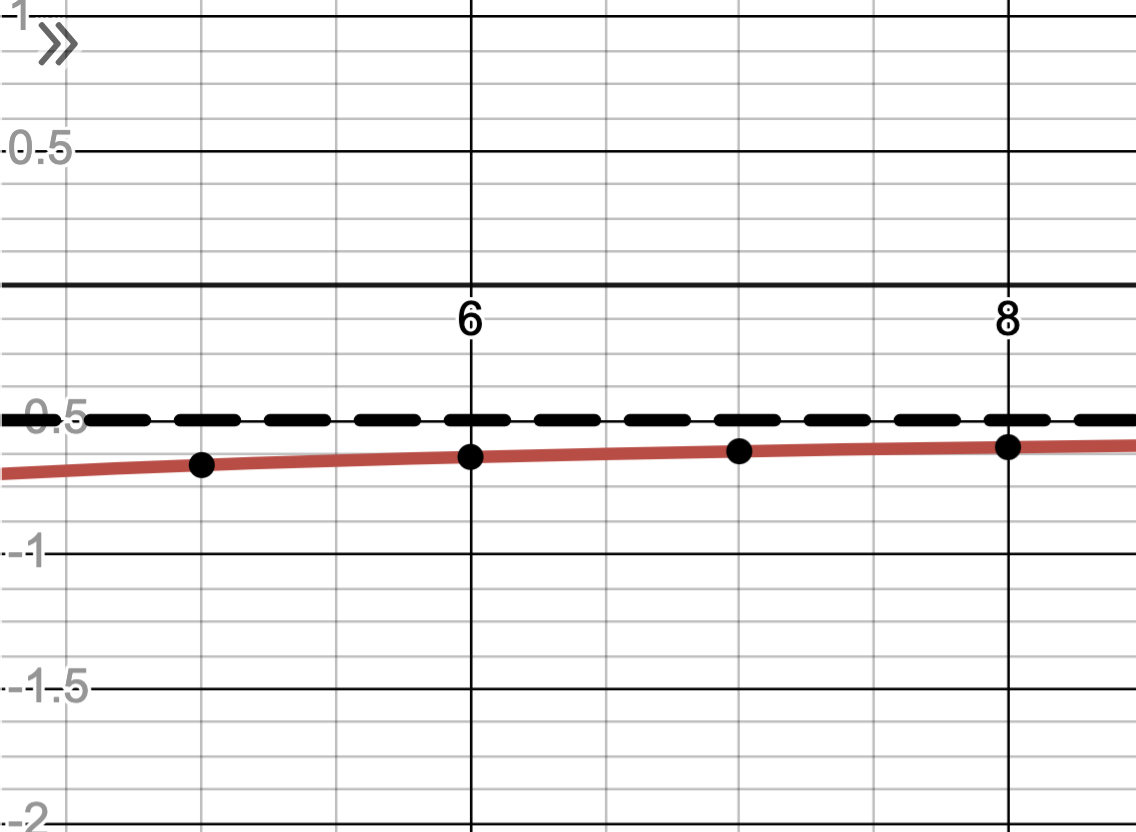
\includegraphics[width=2.5in]{./SequenceGraphics/seqlimitex02.png}

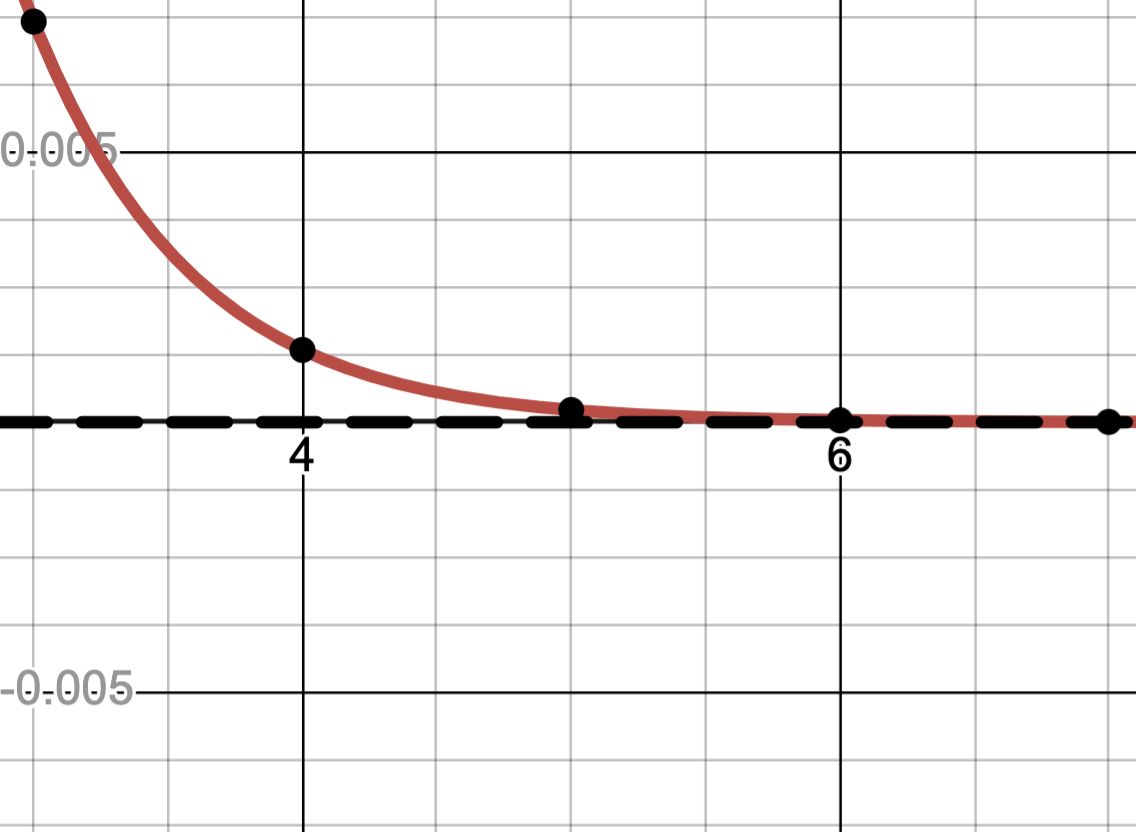
\includegraphics[width=2.5in]{./SequenceGraphics/seqlimitex01.png}

\end{multicols}

\begin{multicols}{2}
$a_{n} = \frac{1 - n^2}{2n^2-3n+1}$ along with $y =  \frac{1 - x^2}{2x^2-3x+1}$

$a_{n} = n e^{-2n}$ along with $y = x e^{-2x}$

\end{multicols}



\end{center}

\end{enumerate}

\item When passing  $\ds{\lim_{n \rightarrow \infty}}$ $\frac{(-1)^{n}}{n^2 +1}$ to a continuous variable, we get the factor $(-1)^{x}$ which is non-real for several\footnote{Actually, `uncountably infinite' \ldots} real numbers such as $x = \frac{1}{2}$, $x = 117.23$, or $x = 3000 \pi$.  That being said, we note that the factor $(-1)^{n}$ alternates the sign of each term:  $(+)1$ if $n$ is even and $-1$ if $n$ is odd:  $-\frac{1}{2}, \frac{1}{5}, -\frac{1}{10}, \frac{1}{17}, \ldots$.

\medskip

This means that we can bound the sequence we're interested in between two other sequences we know something about:  $-\frac{1}{n^2 + 1} \leq \frac{(-1)^{n}}{n^2 +1} \leq \frac{1}{n^2+1}$.

\medskip

Passing to a continuous variable,  $\ds{\lim_{n \rightarrow \infty}}$ $-\frac{1}{n^2 +1} = $ $\ds{\lim_{x \rightarrow \infty}}$ $-\frac{1}{x^2 +1} =0$ and $\ds{\lim_{n \rightarrow \infty}}$ $\frac{1}{n^2 +1} = $ $\ds{\lim_{x \rightarrow \infty}}$ $\frac{1}{x^2 +1} =0$, so it stands to reason that $\ds{\lim_{n \rightarrow \infty}}$ $\frac{(-1)^{n}}{n^2 +1} = 0$ as well.  We sketch the situation out below.

\begin{center}

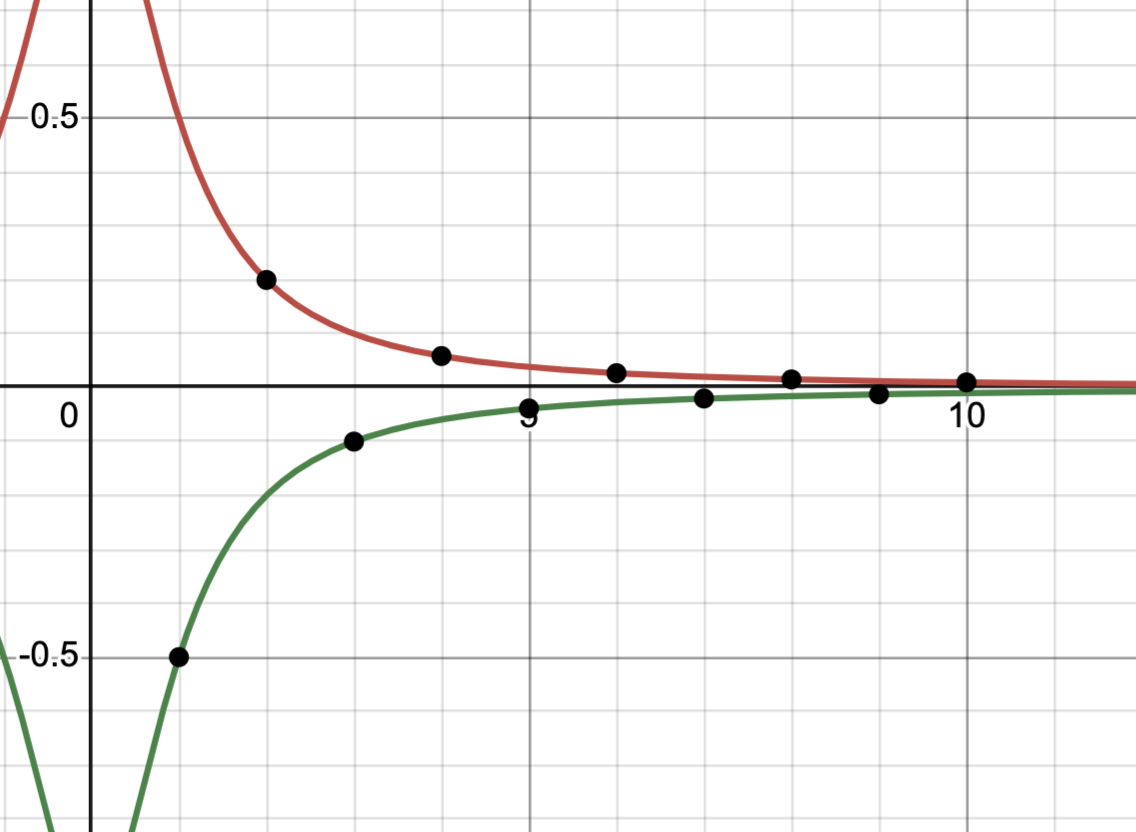
\includegraphics[width=2.5in]{./SequenceGraphics/seqlimitex03.png}

\end{center}

\end{enumerate}


\hfill \qed


\end{ex}

\medskip

The sequence in number \ref{squeezemotivation} in Example \ref{limitofsequenceexample} is an example of an \index{alternating sequence}\index{sequence ! alternating}\textbf{alternating sequence}, so-named because the terms alternate in sign.  Alternating sequences play a large role in the study of infinite series (whatever those are) in Calculus,\footnote{We'll touch on these in the next section, too.}  so it is worth pointing them out here.

\medskip

Next, the reasoning we used to determine  $\ds{\lim_{n \rightarrow \infty}}$ $\frac{(-1)^{n}}{n^2 +1} = 0$ is sound and is codified in the following theorem. We state the result for both sequences (discrete functions) and (continuous) functions.

\medskip



\colorbox{ResultColor}{\bbm

\begin{thm} \label{squeezeth}  \textbf{The Squeeze Theorem:}  $~$

\begin{itemize}

\item Suppose for some natural number $k$, $b_{n} \leq a_{n} \leq c_{n}$ for all $n \geq k$.  

\smallskip

If $\ds{\lim_{n \rightarrow \infty} b_{n} = \lim_{n \rightarrow \infty} c_{n} = L}$, then $\ds{\lim_{n \rightarrow \infty} a_{n} = L}$.

\item Suppose for some real number $M$, $g(x) \leq f(x) \leq h(x)$ for all $x \geq M$.

\smallskip

If $\ds{\lim_{x \rightarrow \infty} g(x) = \lim_{x \rightarrow \infty} h(x) = L}$, then $\ds{\lim_{x \rightarrow \infty} f(x)= L}$.

\end{itemize}

\end{thm}

\ebm}

\medskip

The Squeeze Theorem is so-named because the two sequences (functions) which bound the middle sequence (function) `squeeze' the middle function to the common limit, $L$.

\medskip

\begin{center}

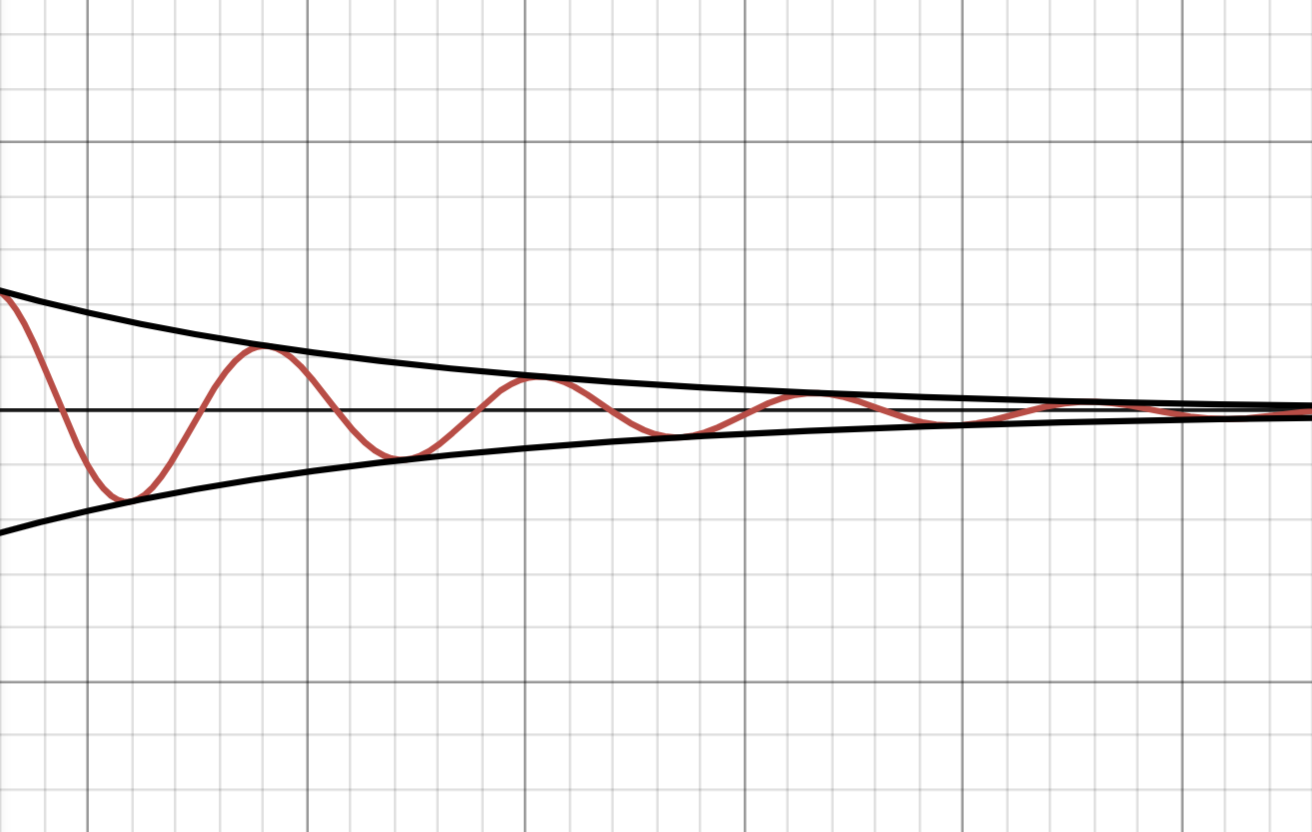
\includegraphics[width=4in]{./SequenceGraphics/squeezethm.png}

The graph of $y = f(x)$ being `squeezed' to a common limit by the graphs of $y = g(x)$  and $y = h(x)$.

\end{center}

Passing to a continuous variable in conjunction with the Squeeze Theorem can be used to prove certain classes of Geometric Sequences converge.  We have the following:

\medskip

\colorbox{ResultColor}{\bbm


\begin{thm}\label{limitsofgeometricsequences}  \textbf{Limits of Geometric Sequences:}  Given a geometric sequence with common ratio $r$:


\begin{enumerate}

\item If $-1 < r < 1$, the sequence converges to $0$.

\medskip

\item If $r=1$, the sequence converges to the first term, $a$.

\medskip

\item If $r> 1$ or $r \leq -1$, the sequence diverges.

\end{enumerate}

\end{thm}

\ebm}

\medskip

We encourage the reader to think through each of the cases stated in Theorem \ref{limitsofgeometricsequences} to make sure the conclusions seem reasonable.  We'll have occasion to cite Theorem \ref{limitsofgeometricsequences} in the next section.  For now, it's time for some Exercises. 


\newpage


\subsection{Exercises}
\documentclass{ximera}

\begin{document}
	\author{Stitz-Zeager}
	\xmtitle{TITLE}
\mfpicnumber{1} \opengraphsfile{ExercisesforSequences} % mfpic settings added 


In Exercises \ref{writeoutseqfirst} - \ref{writeoutseqlast},  write out the first four terms of the given sequence.

\begin{multicols}{2}
\begin{enumerate}


\item $a_{n} = 2^{n} - 1 \vphantom{d_{j} = (-1)^{\dfrac{j(j+1)}{2}}}$, $n \geq 0$  \label{writeoutseqfirst}
\item $d_{j} = (-1)^{\frac{j(j+1)}{2}}$, $j \geq 1$

\setcounter{HW}{\value{enumi}}
\end{enumerate}
\end{multicols}

\begin{multicols}{2}
\begin{enumerate}
\setcounter{enumi}{\value{HW}}

\item $\left\{ 5k - 2 \right\}_{k=1}^{\infty} \vphantom{\left\{ \dfrac{n^2+1}{n+1} \right\}_{n=0}^{\infty}}$
\item $\left\{ \dfrac{n^2+1}{n+1} \right\}_{n=0}^{\infty}$

\setcounter{HW}{\value{enumi}}
\end{enumerate}
\end{multicols}

\begin{multicols}{2}
\begin{enumerate}
\setcounter{enumi}{\value{HW}}

\item $\left\{ \dfrac{x^{n}}{n^{2}} \right\}_{n=1}^{\infty}$
\item $\left\{ \dfrac{\ln(n)}{n} \right\}_{n=1}^{\infty} \vphantom{\left\{ \dfrac{x^{n}}{n^{2}} \right\}_{n=1}^{\infty}}$

\setcounter{HW}{\value{enumi}}
\end{enumerate}
\end{multicols}

\begin{multicols}{2}
\begin{enumerate}
\setcounter{enumi}{\value{HW}}
 
\item  $a_{\mbox{\tiny$1$}} = 3$, $a_{n+\mbox{\tiny$1$}} = a_{n} - 1$, $n \geq 1 \vphantom{d_{m} = \dfrac{d_{m\mbox{-\tiny$1$}}}{100}}$
\item  $d_{\mbox{\tiny$0$}} = 12$, $d_{m} = \dfrac{d_{m\mbox{-\tiny$1$}}}{100}$, $m \geq 1$

\setcounter{HW}{\value{enumi}}
\end{enumerate}
\end{multicols}

\begin{multicols}{2}
\begin{enumerate}
\setcounter{enumi}{\value{HW}}

\item  $b_{\mbox{\tiny$1$}} = 2$, $b_{k\mbox{+\tiny$1$}} =3b_{k}+1 \vphantom{\dfrac{c_{j\mbox{-\tiny$1$}}}{(j+1)(j+2)}}$, $k \geq 1$
\item  $c_{\mbox{\tiny$0$}} = -2$, $c_{j} = \dfrac{c_{j\mbox{-\tiny$1$}}}{(j+1)(j+2)}$,  $j \geq 1$

\setcounter{HW}{\value{enumi}}
\end{enumerate}
\end{multicols}

\begin{multicols}{2}
\begin{enumerate}
\setcounter{enumi}{\value{HW}}

\item  $a_{\mbox{\tiny$1$}} = 117$, $a_{n\mbox{+\tiny$1$}} = \dfrac{1}{a_{n}}$, $n \geq 1$
\item  $s_{\mbox{\tiny$0$}} = 1$, $s_{n\mbox{+\tiny$1$}} = x^{n + 1} + s_{n}$, $n \geq 0$

\setcounter{HW}{\value{enumi}}
\end{enumerate}
\end{multicols}


\begin{enumerate}
\setcounter{enumi}{\value{HW}}

\item  $F_{\mbox{\tiny$0$}} = 1$, $F_{\mbox{\tiny$1$}} = 1$, $F_{n} = F_{n\mbox{-\tiny$1$}} + F_{n\mbox{-\tiny$2$}}$, $n \geq 2$  (This is the famous \href{http://en.wikipedia.org/wiki/Fibonacci_number}{\underline{Fibonacci Sequence}} ) \label{writeoutseqlast}

\setcounter{HW}{\value{enumi}}
\end{enumerate}


In Exercises \ref{alggeoneithfirst} - \ref{alggeoneithlast} determine if the given sequence is arithmetic, geometric or neither.  If it is arithmetic, find the common difference $d$; if it is geometric, find the common ratio $r$.

\begin{multicols}{2}
\begin{enumerate}
\setcounter{enumi}{\value{HW}}

 
\item  $\left\{ 3n-5 \right\}_{n=1}^{\infty}$ \label{alggeoneithfirst}

\item  $a_{n} = n^2+3n+2$, $n \geq 1$

\setcounter{HW}{\value{enumi}}
\end{enumerate}
\end{multicols}


\begin{multicols}{2}
\begin{enumerate}
\setcounter{enumi}{\value{HW}}


\item  $\dfrac{1}{3}$, $\dfrac{1}{6}$, $\dfrac{1}{12}$, $\dfrac{1}{24} \vphantom{\left\{ 3 \left(\dfrac{1}{5}\right)^{n-1} \right\}_{n=1}^{\infty}}$, \ldots

\item  $\left\{ 3 \left(\dfrac{1}{5}\right)^{n-1} \right\}_{n=1}^{\infty}$


\item  $17$, $5$, $-7$, $-19$, \ldots

\item  $2$, $22$, $222$, $2222$, \ldots

\item  $0.9$, $9$, $90$, $900 \vphantom{a_{n} = \dfrac{n!}{2}}$, \ldots

\item  $a_{n} = \dfrac{n!}{2}$, $n \geq 0$.  \label{alggeoneithlast}


\setcounter{HW}{\value{enumi}}
\end{enumerate}
\end{multicols}


In Exercises \ref{nthtermfirst} - \ref{nthtermlast}, find an explicit formula for the $n^{\mbox{\scriptsize th}}$ term of the given sequence.\footnote{Use the formulas in Equation \ref{arithgeoformula} as needed.}

\begin{multicols}{3}
\begin{enumerate}
\setcounter{enumi}{\value{HW}}

\item $3$, $5$, $7$, $9 \vphantom{-\dfrac{1}{8}}$, \ldots \label{nthtermfirst}
\item $1$, $-\dfrac{1}{2}$, $\dfrac{1}{4}$, $-\dfrac{1}{8}$, \ldots
\item $1$, $\dfrac{2}{3}$, $\dfrac{4}{5}$, $\dfrac{8}{7}$, \ldots

\setcounter{HW}{\value{enumi}}
\end{enumerate}
\end{multicols}

\begin{multicols}{3}
\begin{enumerate}
\setcounter{enumi}{\value{HW}}

\item $1$, $\dfrac{2}{3}$, $\dfrac{1}{3}$, $\dfrac{4}{27} \vphantom{\dfrac{x^7}{7}}$, \ldots
\item $1$, $\dfrac{1}{4}$, $\dfrac{1}{9}$, $\dfrac{1}{16} \vphantom{-\dfrac{x^7}{7}}$, \ldots
\item $x$, $-\dfrac{x^3}{3}$, $\dfrac{x^5}{5}$, $-\dfrac{x^7}{7}$, \ldots

\item $0.9, 0.99, 0.999, 0.9999, \ldots$
\item $27, 64, 125, 216, \ldots$
\item $1, 0, 1, 0, \ldots$ \label{nthtermlast}

\setcounter{HW}{\value{enumi}}
\end{enumerate}
\end{multicols}



In Exercises \ref{limseqexfirst} - \ref{limseqexlast}, find the indicated limit by using Theorem \ref{passingtocontinuous} and passing to a continuous variable.\footnote{See Example \ref{limitofsequenceexample}.}


\begin{multicols}{3}
\begin{enumerate}
\setcounter{enumi}{\value{HW}}

\item\label{limseqexfirst}  $\ds{\lim_{n \rightarrow \infty}}$ $\dfrac{2n^2 - 3n+1}{4-n^2}$

\item  $\ds{\lim_{k \rightarrow \infty}}$ $\dfrac{k^2 +7k-3}{3k - k^3}$

\item\label{limseqexlast}  $\ds{\lim_{m \rightarrow \infty}}$ $\dfrac{117m^{42} + 3m + 1}{e^{2m} + 6}$

\setcounter{HW}{\value{enumi}}
\end{enumerate}
\end{multicols}


In Exercises \ref{limsqueezefirst} - \ref{limsqueezelast}, use the Squeeze Theorem,  Theorem \ref{squeezeth} to help you determine the limit.\footnote{See part \ref{squeezemotivation} of Example \ref{limitofsequenceexample}.}


\begin{multicols}{3}
\begin{enumerate}
\setcounter{enumi}{\value{HW}}

\item\label{limsqueezefirst}  $\ds{\lim_{n \rightarrow \infty}}$ $\dfrac{(-1)^{n}}{3n+1}$

\item  $\ds{\lim_{k \rightarrow \infty}}$ $1 - \left( - \frac{2}{3}  \right)^{k} $

\item\label{limsqueezelast}  $\ds{\lim_{m \rightarrow \infty}}$ $\dfrac{(-1)^{ \frac{m^2-m}{2}} }{m!}$

\setcounter{HW}{\value{enumi}}
\end{enumerate}
\end{multicols}





\begin{enumerate}
\setcounter{enumi}{\value{HW}}

\item \label{arithmeticandgeometricexercise} Find a sequence which is both arithmetic and geometric.  (Hint: Start with $a_{n} = c$ for all $n$.)

\item Show that a geometric sequence can be transformed into an arithmetic sequence by taking the natural logarithm of the terms.

\item Thomas Robert Malthus is credited with saying, ``The power of population is indefinitely greater than the power in the earth to produce subsistence for man. Population, when unchecked, increases in a geometrical ratio. Subsistence increases only in an arithmetical ratio. A slight acquaintance with numbers will show the immensity of the first power in comparison with the second.''  (See this \href{http://en.wikipedia.org/wiki/Malthus}{\underline{webpage}} for more information.)  Discuss this quote with your classmates from a sequences point of view.
 
\item This classic problem involving sequences shows the power of geometric sequences.  Suppose that a wealthy benefactor agrees to give you one penny today and then double the amount she gives you each day for 30 days.  So, for example, you get two pennies on the second day and four pennies on the third day.  How many pennies do you get on the $30^{\mbox{\scriptsize th}}$ day?  What is the \underline{total} dollar value of the gift you have received?

\item Research the terms `arithmetic mean' and `geometric mean.'  With the help of your classmates, show that a given term of a arithmetic sequence $a_{k}$, $k \geq 2$ is the arithmetic mean of the term immediately preceding, $a_{k\mbox{\tiny$-1$}}$ it and immediately following it, $a_{k\mbox{\tiny$+1$}}$.  State and prove an analogous result for geometric sequences.  

\item Discuss with your classmates how the results of this section might change if we were to examine sequences of other mathematical things like complex numbers or matrices.  Find an explicit formula for the $n^{\mbox{\scriptsize th}}$ term of the sequence $i, -1, -i, 1, i, \ldots$.  List out the first four terms of the matrix sequences we discussed in Exercise \ref{Markovchain} in Section \ref{MatArithmetic}.



\end{enumerate}

\newpage

\subsection{Answers}

\begin{multicols}{2}
\begin{enumerate}

\item $0, 1, 3, 7$
\item $-1, -1, 1, 1$

\setcounter{HW}{\value{enumi}}
\end{enumerate}
\end{multicols}

\begin{multicols}{2}
\begin{enumerate}
\setcounter{enumi}{\value{HW}}

\item $3, 8, 13, 18$
\item $1, 1, \frac{5}{3}, \frac{5}{2}$

\setcounter{HW}{\value{enumi}}
\end{enumerate}
\end{multicols}

\begin{multicols}{2}
\begin{enumerate}
\setcounter{enumi}{\value{HW}}

\item $x, \frac{x^{2}}{4}, \frac{x^{3}}{9}, \frac{x^{4}}{16}$
\item $0, \frac{\ln(2)}{2}, \frac{\ln(3)}{3}, \frac{\ln(4)}{4}$

\setcounter{HW}{\value{enumi}}
\end{enumerate}
\end{multicols}

\begin{multicols}{2}
\begin{enumerate}
\setcounter{enumi}{\value{HW}}

\item $3, 2, 1, 0$
\item $12, 0.12, 0.0012, 0.000012$

\setcounter{HW}{\value{enumi}}
\end{enumerate}
\end{multicols}

\begin{multicols}{2}
\begin{enumerate}
\setcounter{enumi}{\value{HW}}

\item $2, 7, 22, 67$
\item $-2, -\frac{1}{3}, -\frac{1}{36}, -\frac{1}{720}$

\setcounter{HW}{\value{enumi}}
\end{enumerate}
\end{multicols}

\begin{multicols}{2}
\begin{enumerate}
\setcounter{enumi}{\value{HW}}

\item $117, \frac{1}{117}, 117, \frac{1}{117}$
\item $1, x + 1, x^{2} + x + 1, x^{3} + x^{2} + x + 1 $

\setcounter{HW}{\value{enumi}}
\end{enumerate}
\end{multicols}

\begin{multicols}{2}
\begin{enumerate}
\setcounter{enumi}{\value{HW}}

\item $1, 1, 2, 3$

\setcounter{HW}{\value{enumi}}
\end{enumerate}
\end{multicols}

\begin{multicols}{2}
\begin{enumerate}
\setcounter{enumi}{\value{HW}}

\item  arithmetic, $d = 3$

\item  neither


\setcounter{HW}{\value{enumi}}
\end{enumerate}
\end{multicols}

\begin{multicols}{2}
\begin{enumerate}
\setcounter{enumi}{\value{HW}}

\item  geometric, $r = \frac{1}{2}$

\item  geometric, $r = \frac{1}{5}$

\setcounter{HW}{\value{enumi}}
\end{enumerate}
\end{multicols}

\begin{multicols}{2}
\begin{enumerate}
\setcounter{enumi}{\value{HW}}


\item  arithmetic, $d = -12$

\item  neither

\setcounter{HW}{\value{enumi}}
\end{enumerate}
\end{multicols}

\begin{multicols}{2}
\begin{enumerate}
\setcounter{enumi}{\value{HW}}


\item  geometric, $r = 10$

\item  neither


\setcounter{HW}{\value{enumi}}
\end{enumerate}
\end{multicols}

\begin{multicols}{3}
\begin{enumerate}
\setcounter{enumi}{\value{HW}}

\item $a_{n} = 1 + 2n, \; n \geq 1$
\item $a_{n} = \left(-\frac{1}{2}\right)^{n - 1}, \; n \geq 1$
\item $a_{n} = \frac{2^{n - 1}}{2n - 1}, \; n \geq 1$

\setcounter{HW}{\value{enumi}}
\end{enumerate}
\end{multicols}

\begin{multicols}{3}
\begin{enumerate}
\setcounter{enumi}{\value{HW}}

\item $a_{n} = \frac{n}{3^{n - 1}}, \; n \geq 1$
\item $a_{n} = \frac{1}{n^{2}}, \; n \geq 1$
\item $\frac{(-1)^{n - 1}x^{2n - 1}}{2n -1}, \; n \geq 1$

\setcounter{HW}{\value{enumi}}
\end{enumerate}
\end{multicols}

\begin{multicols}{3}
\begin{enumerate}
\setcounter{enumi}{\value{HW}}

\item $a_{n} = \frac{10^{n} - 1}{10^{n}}, \; n \geq 1$
\item $a_{n} = (n + 2)^{3}, \; n \geq 1$
\item $a_{n} = \frac{1 + (-1)^{n-1}}{2}, \; n \geq 1$
 
\setcounter{HW}{\value{enumi}}
\end{enumerate}
\end{multicols}

\begin{multicols}{3}
\begin{enumerate}
\setcounter{enumi}{\value{HW}}

\item  $\ds{\lim_{n \rightarrow \infty}}$ $\frac{2n^2 - 3n+1}{4-n^2} = -2$

\item  $\ds{\lim_{k \rightarrow \infty}}$ $\frac{k^2 +7k-3}{3k - k^3} = 0$

\item\label{limseqexlast}  $\ds{\lim_{m \rightarrow \infty}}$ $\frac{117m^{42} + 3m + 1}{e^{2m} + 6} = 0$

\setcounter{HW}{\value{enumi}}
\end{enumerate}
\end{multicols}

\begin{multicols}{3}
\begin{enumerate}
\setcounter{enumi}{\value{HW}}

\item  $\ds{\lim_{n \rightarrow \infty}}$ $\frac{(-1)^{n}}{3n+1} = 0$

\item  $\ds{\lim_{k \rightarrow \infty}}$ $1 - \left( - \frac{2}{3}  \right)^{k} = 1$

\item  $\ds{\lim_{m \rightarrow \infty}}$ $\frac{(-1)^{ \frac{m^2-m}{2}} }{m!} = 0$

\setcounter{HW}{\value{enumi}}
\end{enumerate}
\end{multicols}





\end{document}



\closegraphsfile

\end{document}


\newpage

\section{Summation Notation}

\mfpicnumber{1}

\opengraphsfile{Summation}

\setcounter{footnote}{0}

\label{Summation}


In Section \ref{Sequences}, we showed how the formula for compound interest is a geometric sequence.  In retirement planning, it is seldom the case that an investor deposits a set amount of money into an account and waits for it to grow.  Usually, additional payments of principal are made at regular intervals and the value of the investment grows accordingly.  This kind of investment is called an \textit{annuity} and will be discussed in later in this section once we have developed more mathematical machinery that enables us to \textit{add} sequences.


\medskip


In the previous section, we introduced sequences.  Each of the numbers in the sequence is called a `term' which implies these numbers are meant to be added.  To that end, we introduce the following notation which is used to describe  the sum of (some of the) terms of a sequence.
\smallskip

\colorbox{ResultColor}{\bbm

\begin{defn} \textbf{Summation Notation:} \label{sigmanotation} \index{summation notation ! definition of} Given a sequence $\left\{ a_{n} \right\}_{n=k}^{\infty}$ and numbers $m$ and $p$ satisfying $k \leq m \leq p$, the summation from $m$ to $p$ of the sequence $\left\{a_{n}\right\}$ is written  

\[ \sum_{n=m}^{p} a_{n} = a_{m} + a_{m \mbox{\scriptsize$+ 1$}} + \ldots + a_{p}\]

The variable $n$ is called the \index{summation notation ! index of summation} \textbf{index of summation}.   The number $m$ is called the \index{summation notation ! lower limit of summation} \textbf{lower limit of summation} while the number $p$ is called the \index{summation notation ! upper limit of summation} \textbf{upper limit of summation}.

\end{defn}


\ebm}

\smallskip

In English, Definition \ref{sigmanotation} is simply defining a short-hand notation for adding up the terms of the sequence $\left\{ a_{n} \right\}_{n=k}^{\infty}$  from $a_{m}$ through $a_{p}$. The symbol $\Sigma$ is the capital Greek letter sigma and is shorthand for `sum'.  The lower and upper limits of the summation tells us which term to start with and which term to end with, respectively. For example, using the sequence $a_{n} = 2n-1$ for $n \geq 1$, we can write  $a_{\mbox{\scriptsize$3$}} +a_{\mbox{\scriptsize$4$}} + a_{\mbox{\scriptsize$5$}} + a_{\mbox{\scriptsize$6$}}$ as 

\[ \begin{array}{rcl}

\displaystyle{\sum_{n=3}^{6}(2n-1) } & = & (2(3)-1) + (2(4)-1) + (2(5)-1) +  (2(6)-1) \\
                     & = &  5 + 7 + 9 + 11 \\
                     & = & 32 \\
\end{array} \]

The index variable  is considered a `dummy variable' in the sense that it may be changed to any letter without affecting the value of the summation.  For instance, 

\[ \displaystyle{\sum_{n=3}^{6}(2n-1)} = \displaystyle{\sum_{k=3}^{6}(2k-1)} = \displaystyle{\sum_{j=3}^{6}(2j-1)}\]

One place you may encounter summation notation is in mathematical definitions.  For example, summation notation allows us to define polynomials as functions of the form

\[ f(x) = \displaystyle{\sum_{k=0}^{n} a_{k} x^{k}} \]

for real numbers $a_{k}$, $k = 0, 1, \ldots n$.  The reader is invited to compare this with what is given in Definition \ref{polynomialfunction}.  Summation notation is particularly useful when talking about matrix operations.  For example, we can write the product of the $i$th row $R_{i}$ of a matrix $A = [a_{ij}]_{m \times n}$ and the $j^{\mbox{\scriptsize th}}$ column $C_{j}$ of a matrix $B = [b_{ij}]_{n \times r}$ as

\[ Ri \cdot Cj = \displaystyle{\sum_{k=1}^{n} a_{ik}b_{kj}} \]

Again, the reader is encouraged to write out the sum and compare it to Definition \ref{rowcolumnproduct}.  Our next example gives us practice with this new notation. 

\begin{ex} \label{seriesex1} $~$

\begin{enumerate}

\item  Find the following sums.

\begin{multicols}{3}

\begin{enumerate}

\item  $\displaystyle{\sum_{k=1}^{4} \dfrac{13}{100^k} }$

\item  $\displaystyle{\sum_{n=0}^{4} \dfrac{n!}{2}}$

\item  $\displaystyle{\sum_{n=1}^{5} \dfrac{(-1)^{n+1}}{n} (x-1)^n}$

\end{enumerate}

\end{multicols}

\item  Write the following sums using summation notation.

\begin{enumerate}

\item  $1 + 3 + 5 + \ldots + 117$

\item  $1 - \dfrac{1}{2} + \dfrac{1}{3} - \dfrac{1}{4} + - \ldots + \dfrac{1}{117}$

\item  $0.9 + 0.09 + 0.009 + \ldots 0. \! \! \! \! \underbrace{0 \cdots 0}_{\text{$n-1$ zeros}} \! \! \! \! 9$

\end{enumerate}

\end{enumerate}

{ \bf Solution.}

\begin{enumerate}

\item \begin{enumerate} \item We substitute $k=1$ into the formula $\frac{13}{100^k}$ and add successive terms until we reach $k=4.$

\[ \begin{array}{rcl}

\displaystyle{\sum_{k=1}^{4} \dfrac{13}{100^k} } & = & \dfrac{13}{100^1} + \dfrac{13}{100^2} + \dfrac{13}{100^3} + \dfrac{13}{100^4} \\ 
																								& = & 0.13 + 0.0013 + 0.000013 + 0.00000013 \\
																								& = & 0.13131313 \\
\end{array}\]

\item  Proceeding as in (a), we replace every occurrence of $n$ with the values $0$ through $4$.  We recall the factorials, $n!$ as defined in number Example \ref{seqex1}, number \ref{factorialintroex} and get: 

\[ \begin{array}{rcl}

\displaystyle{\displaystyle{\sum_{n=0}^{4} \dfrac{n!}{2}}} & = & \dfrac{0!}{2} + \dfrac{1!}{2} + \dfrac{2!}{2} + \dfrac{3!}{2} = \dfrac{4!}{2} \\ [10pt]
																								& = & \dfrac{1}{2} + \dfrac{1}{2} + \dfrac{2 \cdot 1}{2} + \dfrac{3 \cdot 2 \cdot 1}{2} + \dfrac{4 \cdot 3 \cdot 2 \cdot 1 }{2} \\ [10pt]
																								& = & \dfrac{1}{2} + \dfrac{1}{2} + 1 + 3 + 12 \\ [10pt]
																								& = & 17 \\
\end{array}\]

\item  We proceed as before, replacing the index $n$, but \emph{not} the variable $x$, with the values $1$ through $5$ and adding the resulting terms.

\[ \begin{array}{rcl}

\displaystyle{\sum_{n=1}^{5} \dfrac{(-1)^{n+1}}{n} (x-1)^n} & = &  \dfrac{(-1)^{1+1}}{1} (x-1)^1 + \dfrac{(-1)^{2+1}}{2} (x-1)^2 + \dfrac{(-1)^{3+1}}{3} (x-1)^3 \\ && + \dfrac{(-1)^{1+4}}{4} (x-1)^4 + \dfrac{(-1)^{1+5}}{5} (x-1)^5 \\ [10pt]
& = & (x-1) - \dfrac{(x-1)^2}{2} +  \dfrac{(x-1)^3}{3} -  \dfrac{(x-1)^4}{4} +  \dfrac{(x-1)^5}{5} \\
\end{array} \]

\end{enumerate}

\item  The key to writing these sums with summation notation is to find the pattern of the terms. To that end, we make good use of the techniques presented in Section \ref{Sequences}.

\begin{enumerate}

\item The terms of the sum $1$, $3$, $5$, etc., form an arithmetic sequence with first term $a = 1$ and common difference $d = 2$.  Using Equation \ref{arithgeoformula}, we get $a_{n} = 1 + (n-1)2 = 2n-1$, $n \geq 1$.  

At this stage, we have the formula for the terms, namely $2n-1$, and the lower limit of the summation, $n=1$.  To finish the problem, we need to determine the upper limit of the summation.  In other words, we need to determine which value of $n$ produces the term $117$.  Setting $a_{n} = 117$, we get $2n-1=117$ or $n = 59$.  Our final answer is

\[ \begin{array}{rcl} 1 + 3 + 5 + \ldots + 117 & = & \displaystyle{\sum_{n=1}^{59} (2n-1)} \end{array} \]

\item We rewrite all of the terms as fractions, the subtraction as addition, and associate the negatives `$-$' with the numerators to get

\[ \dfrac{1}{1} + \dfrac{-1}{2} + \dfrac{1}{3} + \dfrac{-1}{4} + \ldots + \dfrac{1}{117}  \]

The numerators, $1$, $-1$, etc. can be described by the geometric sequence\footnote{This is indeed a geometric sequence with first term $a = 1$ and common ratio $r=-1$.} $C_{n} = (-1)^{n-1}$ for $n \geq 1$, while the denominators are given by the arithmetic sequence\footnote{It is an arithmetic sequence with first term $a=1$ and common difference $d=1$.} $D_{n} = n$ for $n \geq 1$.  Hence, we get the formula $a_{n} = \frac{(-1)^{n-1}}{n}$ for our terms, and we find the lower and upper limits of summation to be $n=1$ and  $n = 117$, respectively.  Thus

\[ \begin{array}{rcl} 1 - \dfrac{1}{2} + \dfrac{1}{3} - \dfrac{1}{4} + - \ldots + \dfrac{1}{117} & = & \displaystyle{\sum_{n=1}^{117} \dfrac{(-1)^{n-1}}{n}}   \end{array} \]

\item  Thanks to Example \ref{seqex2}, we know that one formula for the $n^{\mbox{\scriptsize th}}$ term is $a_{n} = \frac{9}{10^{n}}$ for $n \geq 1$.  This gives us a formula for the summation as well as a lower limit of summation.  

To determine the upper limit of summation, we note that to produce the $n-1$ zeros to the right of the decimal point before the $9$, we need a denominator of $10^{n}$.  Hence, $n$ is the upper limit of summation.  

Since $n$ is used in the limits of the summation, we need to choose a different letter for the index of summation.\footnote{To see why, try writing the summation using `$n$' as the index.}  We choose $k$ and get

  
\[ \begin{array}{rcl} 0.9 + 0.09 + 0.009 + \ldots 0.\! \! \! \! \underbrace{0 \cdots 0}_{\text{$n-1$ zeros}} \! \! \! \! 9 & = & \displaystyle{\sum_{k=1}^{n} \dfrac{9}{10^{k}}} \end{array} \]

\qed

\end{enumerate}

\end{enumerate}
                    
\end{ex}          

The following theorem presents some general properties of summation notation. 

\smallskip

\colorbox{ResultColor}{\bbm

\begin{thm}  \label{sigmaprops} \textbf{Properties of Summation Notation:} Suppose $\left\{a_{n}\right\}$ and $\left\{b_{n}\right\}$ are sequences so that the following sums are defined. \index{summation notation ! properties of}

\begin{itemize}

\item \textbf{Sum and Difference Property:} $\displaystyle{ \sum_{n=m}^{p} \left(a_{n} \pm b_{n} \right) =  \sum_{n=m}^{p} a_{n} \pm \sum_{n=m}^{p} b_{n} }$

\item \textbf{Distributive Property:} $\displaystyle{\sum_{n=m}^{p} c \, a_{n} = c \sum_{n=m}^{p} a_{n}}$, for any real number $c$.

\item \textbf{Additive Index Property:} $\displaystyle{\sum_{n=m}^{j} a_{n} + \sum_{n=j+1}^{p} a_{n} = \sum_{n=m}^{p}  a_{n}}$, for any natural number $m \leq j < j+1 \leq p$.

\item \textbf{Re-indexing:} $\displaystyle{\sum_{n=m}^{p} a_{n} = \sum_{n=m+r}^{p+r} a_{n-r}}$, for any integer $r$.

\end{itemize}

\end{thm}

\ebm}

\smallskip


There is much to be learned by thinking about why the properties hold, so we leave the proof of these properties to the reader.\footnote{To get started, remember the mantra ``When in doubt, write it out!''}  


\begin{ex}  \label{summationpropsex}  $~$

\begin{enumerate}

\item  If $\displaystyle{ \sum_{n=2}^{50}  \left(a_{n}  - 3 b_{n} \right) = 17}$ and $\displaystyle{ \sum_{n=2}^{50}  a_{n}  = 10}$, find $\displaystyle{ \sum_{n=2}^{50}  b_{n}}$.

\item If $\displaystyle{ \sum_{n=1}^{20}  a_{n}  = -3}$ and $\displaystyle{ \sum_{n=1}^{21}  a_{n}  = 7}$, find $a_{21}$.

\item  Rewrite the sum so the index starts at $0$: $\displaystyle{ \sum_{n=2}^{437} n (n-1) x^{n-2}}$


\end{enumerate}

{\bf Solution.}

\begin{enumerate}

\item Using the Sum and Difference Property along with the Distributive Property  of Theorem \ref{sigmaprops}, we get:

\[  \sum_{n=2}^{50}  \left(a_{n}  - 3 b_{n} \right) =  \sum_{n=2}^{50}  a_{n}  -  \sum_{n=2}^{50} 3 b_{n}  = \sum_{n=2}^{50}  a_{n}  - 3 \sum_{n=2}^{50} b_{n}\]

Hence,$\displaystyle{\sum_{n=2}^{50}  a_{n}  - 3 \sum_{n=2}^{50} b_{n} = 17}$. If $\displaystyle{ \sum_{n=2}^{50}  a_{n}  = 10}$, then $\displaystyle{10  - 3 \sum_{n=2}^{50} b_{n} = 17}$ so  $\displaystyle{\sum_{n=2}^{50} b_{n} = -\frac{7}{3}}$.

\item  There are at least two ways to approach this problem.  By definition,  $\displaystyle{ \sum_{n=1}^{21}  a_{n} = a_{1} + a_{2} + \ldots + a_{21}}$.  That is, we add up the first $21$ terms of the sequence $a_{n}$.  Similarly, $\displaystyle{ \sum_{n=1}^{20}  a_{n} = a_{1} + a_{2} + \ldots + a_{20}}$ means we add up the first $20$ terms of the sequence.  Hence, $a_{21} = \displaystyle{ \sum_{n=1}^{21}  a_{n}  - \sum_{n=1}^{20}  a_{n}  = 7-(-3) = 10.}$

Alternatively, we can use the Additive Index Property: 

\[ \sum_{n=1}^{21}  a_{n} = \sum_{n=1}^{20}  a_{n} + \sum_{n=21}^{21}  a_{n} =  \sum_{n=1}^{20}  a_{n}  + a_{21},\]

which gives  $a_{21} = \displaystyle{ \sum_{n=1}^{21}  a_{n}  - \sum_{n=1}^{20}  a_{n}  = 7-(-3) = 10}$ as well.

\item To re-index $\displaystyle{ \sum_{n=2}^{437} n (n-1) x^{n-2}}$ so $n$ starts at $0$,  we follow the formula in Theorem \ref{summationpropsex}  with $r=-2$:  \[ \sum_{n=2}^{437} n (n-1) x^{n-2} =  \sum_{n=2+(-2)}^{437+(-2)} (n-(-2)) (n-(-2)-1) x^{n -(-2) -2} = \sum_{n=0}^{435} (n+2) (n+1) x^{n}. \]  We leave it to the reader to check by writing out the first few, and last few, terms.

Alternatively, to better see \textit{why} the re-indexing works in this way, we can introduce a new counter, $k$.  We want this new counter to start at $k =0$ whereas the current counter starts at $n=2$, so we want $k = n-2$.   When $n=2$, $k=0$, as required, and when $n=437$, $k = 435$.  

Moreover, $n = k+2$, so substituting this into the sum, we get 

 \[ \sum_{n=2}^{437} n (n-1) x^{n-2} =  \sum_{k=0}^{435} (k+2) ((k+2)-1) x^{(k+2) -2} = \sum_{k=0}^{435} (k+2) (k+1) x^{k}, \] 

which is the same sum we had before, just with a different dummy variable. \qed

\end{enumerate}


\end{ex}


We now turn our attention to the sums involving arithmetic and geometric sequences. Given an arithmetic sequence $a_{k} = a + (k-1) d$ for $k \geq 1$, we let $S$ denote the sum of the first $n$ terms. To derive a formula for $S$, we write it out in two different ways \[ \begin{array}{ccccccccccc}

S & = & a & + & (a + d) &  + & \ldots & + & (a + (n-2)d) & + & (a + (n-1)d) \\ 

S & = & (a + (n-1)d) & + & (a + (n-2)d)  & + & \ldots & + & (a + d)  & + & a \\

\end{array}\] If we add these two equations and combine the terms which are aligned vertically, we get 

\[2S = (2a + (n-1)d) + (2a + (n-1)d) + \ldots + (2a + (n-1)d) + (2a + (n-1)d)\]


The right hand side of this equation contains $n$ terms, all of  which are equal to $(2a + (n-1)d)$ so we get $2S = n(2a + (n-1)d)$.  Dividing both sides of this equation by $2$, we obtain the formula

\[S =  \dfrac{n}{2} (2a + (n-1)d)\]

If we rewrite the quantity $2a + (n-1)d$ as $a + (a + (n-1)d) = a_{\mbox{\scriptsize$1$}} + a_{n}$, we get the formula 

\[ S = n \left(\dfrac{a_{\mbox{\scriptsize$1$}} + a_{n}}{2}\right)\]

A helpful way to remember this last formula is to recognize that we have expressed the sum as the product of the number of terms $n$ and the \textit{average} of the first and $n^{\mbox{\scriptsize th}}$ terms.

\smallskip

To derive the formula for the geometric sum, we start with a geometric sequence $a_{k} = ar^{k-1}$, $k \geq 1$, and let $S$ once again denote the sum of the first $n$ terms.  Comparing  $S$ and $rS$, we get

\[ \begin{array}{ccccccccccccccc}

S & = & a & + & ar &  + & ar^2 & + & \ldots & + & ar^{n-2} & + & ar^{n-1} & & \\ 

r S & = & & & ar & + & ar^2 & + & \ldots &  + & ar^{n-2} & + & ar^{n-1} & + & ar^{n}  \\

\end{array}\]

Subtracting the second equation from the first forces all of the terms except $a$ and $ar^{n}$ to cancel out and we get $S - rS = a - ar^{n}$.  Factoring, we get $S(1-r) = a \left(1-r^{n}\right)$.  Assuming $r \neq 1$, we can divide both sides by  the quantity $(1-r)$ to obtain

\[S =  a \left( \dfrac{1-r^n}{1-r}\right)\]

If we distribute $a$ through the numerator, we get $a - ar^{n} = a_{\mbox{\scriptsize$1$}} - a_{n\mbox{\scriptsize$ + 1$}}$ which yields the formula

\[S =  \dfrac{a_{\mbox{\scriptsize$1$}}-a_{n\mbox{\scriptsize$ + 1$}}}{1-r}\]

In the case when $r=1$, we get the formula

\[ S = \underbrace{a + a + \ldots +a }_{\text{$n$ times}} = n \, a\]

Our results are summarized below.\footnote{Alternatively, we can use Exercise \ref{geoseriespreview} in Section \ref{Polydivision}.}


\smallskip

\colorbox{ResultColor}{\bbm

\begin{eqn}  \label{arithgeosum}  \textbf{Sums of Arithmetic and Geometric Sequences:}

\begin{itemize}

\item  The sum $S$ of the first $n$ terms of an arithmetic sequence $a_{k}= a + (k-1)d$ for $k \geq 1$ is 

\[ S = \displaystyle{\sum_{k=1}^{n} a_{k}} = n \left(\dfrac{a_{\mbox{\scriptsize$1$}} + a_{n}}{2}\right) = \dfrac{n}{2} (2a + (n-1)d)\]


\item  The sum $S$ of the first $n$ terms of a geometric sequence $a_{k}= ar^{k-1}$ for $k \geq 1$ is 

\begin{enumerate}

\item $S = \displaystyle{\sum_{k=1}^{n} a_{k}} = \dfrac{a_{\mbox{\scriptsize$1$}} - a_{n\mbox{\scriptsize$ + 1$}}}{1-r} =a \left( \dfrac{1-r^n}{1-r}\right)$, if $r \neq 1$. \index{sequence ! arithmetic ! sum of first $n$ terms}

\item $S = \displaystyle{\sum_{k=1}^{n} a_{k} = \sum_{k=1}^{n} a =n a}$, if $r =1$. \index{sequence ! geometric ! sum of first $n$ terms}

\end{enumerate}

\end{itemize}

\end{eqn}

\ebm}

\smallskip

While we have made an honest effort to derive the formulas in Equation \ref{arithgeosum}, formal proofs require the machinery in Section \ref{Induction}.   

\begin{ex} \label{arithgeosumex} $~$

\begin{enumerate}

\item

\begin{enumerate}
\item  Find the sum: $1 + 3 + 5 + \ldots + 117$

\item Find a formula for the sum $\displaystyle{ \sum_{k=1}^{n} k }$.

\end{enumerate}

\item  The classic \href{https://en.wikipedia.org/wiki/Wheat_and_chessboard_problem}{\underline{wheat and chessboard problem}} asks the following question.  Given a chessboard with its squares numbered $1$ to $64$, suppose  on the first square was placed one grain of wheat, the second square, two grains, the third square, four grains, and so on, each square receiving twice the number of grains as its predecessor.   How many total grains of wheat would end up on the chessboard?

\end{enumerate}

{\bf Solution.}


\begin{enumerate}
\item 
\begin{enumerate}

\item Recognizing the terms of $1 + 3 + 5 + \ldots + 117$ as $1$, $3$, $5$, and so on, we see we have an arithmetic sequence with $a=1$ and $d=2$.  Using Equation \ref{arithgeoformula}, we get a formula for the terms  $a_{n} = 1 + 2(n-1) = 2n-1$ for $n \geq 1$.  In order to use the formula in Equation \ref{arithgeosum}, we need to determine the number of terms being added, $n$.  Setting $2n-1 = 117$, we find $n = 59$.  Feeding in all of our data into Equation \ref{arithgeosum}, we get $1 + 3 + 5 + \ldots + 117 =59 \left(\frac{1+117}{2}\right) = 3481$. 
 
\item Applying the adage `when in doubt, write it out,' we have $\displaystyle{ \sum_{k=1}^{n} k  = 1 + 2 + 3 + 4 + \ldots + n}$.  We see the terms here form an arithmetic sequence with  $a = d = 1$.  Moreover, we are adding exactly $n$ terms, so  Equation \ref{arithgeosum} gives  $\displaystyle{ \sum_{k=1}^{n} k  = 1 + 2 + 3 + 4 + \ldots + n = \dfrac{n(n+1)}{2}}$.

As a side note, the special case:  $1 + 2 + 3 + \ldots + 100$ was allegedly given to  \href{http://en.wikipedia.org/wiki/Carl_Friedrich_Gauss}{\underline{Carl  Friedrich Gauss}}  while he was in  elementary school.  Instead of computing the sum in a brute force method, he arrived at the answer by grouping $1+99 = 100$, $2+98 = 100$, etc.  so that he had $50$ groups of $100$ with $50$ left over for a total of $5050$.  This is the exact same methodology we used to prove the sum of the arithmetic sequence formula in Equation \ref{arithgeosum}.

\end{enumerate}

\item Since we are \textit{doubling} the number of grains of wheat as we move from one square to the next, a geometric sequence with $r=2$ describes the number of grains on each individual square.  

Since we start with one grain on the first square, the number of grains on the $k$th square is $a_{k} = (1) (2)^{k-1} = 2^{k-1}$ for $k \geq 1$.  

Adding up the number of grains on each square gives:

\[1 + 2 + \ldots + 2^{64-1} = 1 + 2 + \ldots 2^{63} = \dfrac{1-2^{64}}{1-2} = 2^{64} - 1 \approx 1.8 \times 10^{19},\] 

in accordance with Equation \ref{arithgeosum}. (The weight of these grains would total approximately $2.6 \times 10^{15}$ pounds which is approximately $15$ times the entire biomass of the planet.) \qed

\end{enumerate}

\end{ex}


\smallskip

An important application of the geometric sum formula is the investment plan called an \index{annuity ! ordinary ! definition of} \textit{annuity}. Annuities differ from the kind of investments we studied in Section \ref{ExpLogApplications} in that payments are deposited into the account on an on-going basis, and this complicates the mathematics a little.\footnote{The reader may wish to re-read the discussion on compound interest in Section \ref{ExpLogApplications} before proceeding.} 


Suppose you have an account with annual interest rate $r$ which is compounded $n$ times per year.  We let $i = \frac{r}{n}$ denote the interest rate  per period.  Suppose we wish to make ongoing deposits of $P$ dollars at the \textit{end} of each compounding period.  Let $A_{k}$ denote the amount in the account after $k$ compounding periods.  

Then $A_{\mbox{\scriptsize$1$}} = P$, because we have  made our first deposit at the \textit{end} of the first compounding period and no interest has been earned.  During the second compounding period, we earn interest on $A_{\mbox{\scriptsize$1$}}$ so that our initial investment has grown to $A_{\mbox{\scriptsize$1$}}(1+i) = P(1+i)$ in accordance with Equation \ref{simpleinterest}.  Adding our second payment at the end of the second period, we get

\[A_{\mbox{\scriptsize$2$}} = A_{\mbox{\scriptsize$1$}}(1+i) + P = P(1+i) + P = P(1+i)\left(1 + \dfrac{1}{1+i}\right)\]

The reason for factoring out the $P(1+i)$ will become apparent in short order. During the third compounding period, we earn interest on $A_{\mbox{\scriptsize$2$}}$ which then grows to $A_{\mbox{\scriptsize$2$}}(1+i)$.  We add our third payment at the end of the third compounding period to obtain

\[A_{\mbox{\scriptsize$3$}} = A_{\mbox{\scriptsize$2$}}(1+i) + P = P(1+i)\left(1 + \dfrac{1}{1+i}\right)(1+i) + P = P(1+i)^2\left(1 + \dfrac{1}{1+i} + \dfrac{1}{(1+i)^2}\right)\]

During the fourth compounding period, $A_{\mbox{\scriptsize$3$}}$ grows to $A_{\mbox{\scriptsize$3$}}(1+i)$, and when we add the fourth payment, we factor out $P(1+i)^3$ to get

\[A_{\mbox{\scriptsize$4$}} = P(1+i)^3 \left(1 + \dfrac{1}{1+i} + \dfrac{1}{(1+i)^2} + \dfrac{1}{(1+i)^3}\right)\]

This pattern continues so that at the end of the $k$th compounding, we get 

\[A_{k} = P(1+i)^{k-1} \left(1 + \dfrac{1}{1+i} + \dfrac{1}{(1+i)^2} + \ldots + \dfrac{1}{(1+i)^{k-1}}\right) \]

The sum in the parentheses above is the sum of the first $k$ terms of a geometric sequence with $a = 1$ and $r = \frac{1}{1+i}$.  Using Equation \ref{arithgeosum}, we get

\[1 + \dfrac{1}{1+i} + \dfrac{1}{(1+i)^2} + \ldots + \dfrac{1}{(1+i)^{k-1}} = 1 \left(\dfrac{1 - \dfrac{1}{(1+i)^k}}{1 - \dfrac{1}{1+i}}\right) = \
\dfrac{(1+i)\left(1 - (1+i)^{-k}\right)}{i}\]

Hence, we get

\[A_{k} = P(1+i)^{k-1} \left(\dfrac{(1+i)\left(1 - (1+i)^{-k}\right)}{i}\right) = \dfrac{P\left((1+i)^k - 1\right)}{i}\]

If we let $t$ be the number of years this investment strategy is followed, then $k = nt$, and we get the formula for the future value of an \index{annuity ! ordinary ! future value} \textit{ordinary annuity}.

\smallskip

\colorbox{ResultColor}{\bbm

\begin{eqn}  \label{fvannuity}  \textbf{Future Value of an Ordinary Annuity:}  Suppose an annuity offers an annual interest rate $r$ compounded $n$ times per year. Let $i = \frac{r}{n}$ be the interest rate per compounding period. If a deposit $P$ is made at the end of each compounding  period, the amount $A$ in the account after $t$ years is given by

\[A = \dfrac{P\left((1+i)^{nt} - 1\right)}{i}\]

\end{eqn}

\ebm}

\smallskip

The reader is encouraged to substitute  $i = \frac{r}{n}$ into Equation \ref{fvannuity} and simplify.  Some familiar equations arise which are cause for pause and meditation.  One last note: if the deposit $P$ is made a the \textit{beginning} of the compounding period instead of at the end, the annuity is called an \index{annuity ! annuity-due} \textit{annuity-due}.  We leave the derivation of the formula for the future value of an annuity-due as an exercise for the reader.


\begin{ex} \label{annuityex}  An ordinary annuity offers a $6 \%$ annual interest rate, compounded monthly.

\begin{enumerate}

\item  If monthly payments of $\$50$ are made, find the value of the annuity in $30$ years.

\item  How many  years will it take for the  annuity to grow to  $\$100,\! 000$?

\end{enumerate}

{\bf Solution.}

\begin{enumerate}

\item We have $r = 0.06$ and $n = 12$ so that $i = \frac{r}{n} = \frac{0.06}{12} = 0.005$.  With $P=50$ and  $t=30$,  

\[A = \dfrac{50\left((1+0.005)^{(12)(30)} - 1\right)}{0.005} \approx  50225.75\]

Our final answer is $\$50,\!225.75$.

\item To find how long it will take for the annuity to grow to $\$100,\!000$, we set $A = 100000$ and solve for $t$.  We isolate the exponential and take natural logs of both sides of the equation.

\[ \begin{array}{rcl}

100000 & = &  \dfrac{50\left((1+0.005)^{12t} - 1\right)}{0.005} \\ [10pt]

10 & = &  (1.005)^{12t} - 1 \\  [4pt]

(1.005)^{12t} & = &  11 \\ [4pt]

\ln\left((1.005)^{12t}\right) & = & \ln(11) \\ [4pt]

12t \ln(1.005) & = & \ln(11) \\ [4pt]

t & = & \frac{\ln(11)}{12 \ln(1.005)} \approx 40.06 \\

\end{array} \]

This means that it takes just over $40$ years for the investment to grow to $\$100,\!000$.  Comparing this with our answer to part 1, we see that in just $10$ additional years, the value of the annuity nearly doubles. This is a lesson worth remembering.  \qed 

\end{enumerate}

\end{ex}

\subsection{Geometric Series}
\label{GeometricSeries}

As defined in Section \ref{Sequences}, sequences are an \textit{infinite} list of numbers.  So far in this section, we have concerned ourselves with adding only \textit{finitely} many terms.   In Calculus,  \textit{infinite} sums, called \index{series}\index{infinite series}\index{series ! infinite}\textbf{series} are studied at great length.  While we do not have the mathematical machinery to embark upon an exhaustive study here, we can nevertheless focus our attention on what is arguably one of the most prevalent and useful types of series, \index{geometric series}\index{series ! geometric}\textbf{geometric series}.

As a motivating example, consider the number $0.\overline{9}$.  We can write this number as

\[ 0.\overline{9} = 0.9999... = 0.9 + 0.09 + 0.009 + 0.0009 + \ldots \]


From Example \ref{seriesex1}, we know we can write the sum of the first $n$ of these terms as 

\[ 0.\underbrace{9 \cdots 9}_{\text{$n$ nines}} = .9 + 0.09 + 0.009 + \ldots 0.\! \! \! \! \underbrace{0 \cdots 0}_{\text{$n-1$ zeros}} \! \! \! \! 9 = \displaystyle{\sum_{k=1}^{n} \dfrac{9}{10^{k}}} \]

Using Equation \ref{arithgeosum}, we have


\[\displaystyle{\sum_{k=1}^{n} \dfrac{9}{10^{k}}} = \sum_{k=1}^{n} \dfrac{9}{10} \left(\dfrac{1}{10^{k-1}}\right) = \sum_{k=1}^{n} \dfrac{9}{10} \left(\dfrac{1}{10}\right)^{k-1} =  \dfrac{9}{10} \left( \dfrac{1 - \dfrac{1}{10^{n}}}{1 - \dfrac{1}{10}} \right) = 1 - \dfrac{1}{10^{n}}   \]

It stands to reason that we should define $0.\overline{9} = \ds{\lim_{n \rightarrow \infty}}$ $\left(1 - \frac{1}{10^{n}}\right)$.  Passing to a continuous variable along with our knowledge of exponential functions  gives  $\ds{\lim_{n \rightarrow \infty}}$ $\left(1 - \frac{1}{10^{n}} \right) =$ $\ds{\lim_{x \rightarrow \infty}}$ $\left(1 - \frac{1}{10^{x}} \right) = 1 - 0 = 1$.

\medskip

We have just argued that $0.\overline{9} = 1$, which may shock some readers.\footnote{To make this more palatable, it is usually accepted that $0.\overline{3} = \frac{1}{3}$ so that $0.\overline{9} = 3\left(0.\overline{3}\right) = 3\left(\frac{1}{3} \right) = 1$.}  

Note that in this manner, any non-terminating decimal can be thought of as an infinite sum whose denominators are the powers of $10$, so the phenomenon of adding up infinitely many terms and arriving at a finite number is not as foreign of a concept as it may appear. We have the following theorem.

\medskip

\colorbox{ResultColor}{\bbm

\begin{thm}  \label{geoseries} \textbf{Geometric Series:} Given the sequence $a_{k} = ar^{k-1}$ for $k \geq 1$, where $|r| < 1$,

\[ a + ar + ar^2 + \ldots = \displaystyle{\sum_{k=1}^{\infty} ar^{k-1}} = \displaystyle{\lim_{n \rightarrow \infty} \sum_{k=1}^{n} ar^{k-1}} =  \dfrac{a}{1-r}\]

If $|r| \geq 1$, the sum $a + ar + ar^2 + \ldots $ does not exist. \index{geometric series}

\end{thm}

\ebm}

\smallskip

The justification of the result in Theorem \ref{geoseries} comes from taking the formula in Equation \ref{arithgeosum} for the sum of the first $n$ terms of a geometric sequence and taking the limit as $n \rightarrow \infty$.  

Assuming $|r|<1$ means $-1 < r < 1$, so per Theorem \ref{limitsofgeometricsequences},  $\ds{\lim_{n \rightarrow \infty}}$ $r^{n} =  0$.  Using this fact along with the Limit Properties listed in Theorem \ref{LimitProp01}:

\[\displaystyle{\lim_{n \rightarrow \infty} \sum_{k=1}^{n} a r^{k-1}} = \lim_{n \rightarrow \infty}  a \left( \dfrac{1-r^n}{1-r}\right) =  \dfrac{a}{1-r} \]

We'll explore what goes wrong when $|r| \geq 1$ in some of the Exercises. For now, we put this theorem to good use in the following example.

\begin{ex} \label{geoseriesex} $~$

\begin{enumerate}

\item  Find the sum: $\dfrac{1}{2} + \dfrac{1}{4}  + \dfrac{1}{8} + \ldots$.  

\item Represent $4.2\overline{17}$ as a fraction in lowest terms. 

\end{enumerate}

{\bf Solution.}

\begin{enumerate}

\item  We recognize $\dfrac{1}{2} + \dfrac{1}{4}  + \dfrac{1}{8} + \ldots$ as a geometric series with $a = r = \frac{1}{2}$.  Using Theorem \ref{geoseries}, we get \[\dfrac{1}{2} + \dfrac{1}{4}  + \dfrac{1}{8} + \ldots = \dfrac{\frac{1}{2}}{1 - \frac{1}{2}} = 1.\]  The interested reader is invited to research this sum as it relates to  \href{https://en.wikipedia.org/wiki/Zeno's_paradoxes}{\underline{Zeno's Dichotomy Paradox}}.

\item  To use  Theorem \ref{geoseries} as it applies to the repeating decimal $4.2\overline{17}$, we first need to rewrite this decimal in terms of a geometric series.  Expanding  $4.2\overline{17} = 4.2 + 0.017 + 0.00017 + 0.0000017 + \ldots,$ we see the series $0.017 + 0.00017 + 0.0000017 + \ldots$ is geometric with $a = 0.017$ and $r = 0.01$.  Hence, we can apply Theorem \ref{geoseries} to that part of the decimal to get:

\[ 0.017 + 0.00017 + 0.0000017 + \ldots = \dfrac{0.017}{1 - 0.01} = \dfrac{\frac{17}{1000}}{\frac{99}{100}} = \frac{17}{990} \]

Hence, $4.2\overline{17} = 4.2 + \dfrac{17}{990} = \dfrac{42}{10} + \dfrac{17}{990} = \dfrac{835}{198}$. \qed

\end{enumerate}

\end{ex}

We note that another popular method for converting repeating decimals to fractions goes something like this:  let $x =4.2\overline{17}$. Then, $100x = 421.7\overline{17}$.  Hence, $99x = 100x - x = 421.7\overline{17} - 4.2\overline{17} = 417.5$.  Hence,  $x = \frac{417.5}{99}  = \frac{835}{198}$.  While this procedure results in the same (correct!) answer, the manipulations involved (such as the multiplication and subtraction) are actually using some of the properties listed in Theorem \ref{sigmaprops}  extended to infinite sums via Theorem \ref{LimitProp01}.


\subsection{Area}
\label{AreabySum}

One of the (two) major geometric problems studied in Calculus is finding the area under a curve\footnote{The other is the concept of tangent lines which we touch on (awesome pun!) in Section \ref{IntroductiontoDerivatives}.}  (more specifically, the area between the graph of a function and the $x$-axis.)\footnote{The area can actually represent a wide variety of things such as displacement, probability, or, as odd as it sounds, volume.}  In this section, we explore how summation notation is used to help better formulate this problem, and, as with our study of Geometric Series, sneak a peak into Calculus itself.

\medskip

Suppose we wish to determine the area between the graph of a continuous function $y = f(x)$  over the interval  $[a,b]$ and the $x$-axis as shown below on the left.  Since we don't know any area formulas for arbitrary regions, we stick to what we know - rectangles.  

\medskip

To keep things simple, we  divide $[a,b]$ into $n$ equal pieces (subintervals), and use the right-endpoints of each piece to determine the height of the rectangles.\footnote{In Calculus, you'll also use left endpoints and midpoints \ldots.}  We let $x_{k}$ represent the right endpoint of the $k$th subinterval, so the height of the $k$th rectangle is $f(x_{k})$.  

\medskip

The width of the $k$th rectangle is the length of the $k$th subinterval.  Since the interval itself is $b-a$ units long and we are dividing the interval into $n$ \textit{equal} pieces, each piece is $\frac{b-a}{n}$  units long.  For brevity, we'll call this length  `$\Delta x$.'   Below on the right is a depiction of $RS_{\, 7}$, a `right endpoint sum' using $7$ (equally spaced) subintervals.\footnote{On intervals over which the function is \textit{increasing}, we find the area of rectangles \textit{overestimates} the area we want;  on intervals over which the function is \textit{decreasing}, we find the area of the rectangles \textit{underestimates} the area we want.}

\begin{center}
\begin{multicols}{2}
\begin{mfpic}[20]{-1}{9}{-1}{4}
 \fillcolor[gray]{0.7}
 \gfill \btwnfcn{1,8,0.1}{0}{cos(3.14159*x/4-3.14159/4)+ 2.5}
\axes
\tlabel[cc](0.5,4){\scriptsize $y$}
\tlabel[cc](9, -0.5){\scriptsize $x$}
\xmarks{1,2,3,4,5,6,7,8}
\tlpointsep{4pt}
\axislabels {x}{{\scriptsize $a=x_{0}$} 1, {\scriptsize $x_{1}$} 2, {\scriptsize $x_{2}$} 3, {\scriptsize $x_{3}$} 4, {\scriptsize $x_{4}$} 5, {\scriptsize $x_{5}$} 6, {\scriptsize $x_{6}$} 7, {\scriptsize $x_{7}=b$} 8}
\penwd{1.25pt}
 \function{1, 8, 0.1}{cos(3.14159*x/4-3.14159/4)+ 2.5}
 \polyline{(1,0), (1,3.5)}
 \polyline{(8,0), (8,3.2)}
 \point[4pt]{(1, 3.5), (8, 3.2)}
 
\tcaption{Area under the graph of $y = f(x)$}
 
\end{mfpic}


\begin{mfpic}[20]{-1}{9}{-1}{4}
 \fillcolor[gray]{0.7}
 \gfill \btwnfcn{1,2,0.1}{0}{3.2}
 \gfill \btwnfcn{2,3,0.1}{0}{2.5}
 \gfill \btwnfcn{3,4,0.1}{0}{1.79}
 \gfill \btwnfcn{4,5,0.1}{0}{1.5}
 \gfill \btwnfcn{5,6,0.1}{0}{1.79}
\gfill \btwnfcn{6,7,0.1}{0}{2.5}
\gfill \btwnfcn{7,8,0.1}{0}{3.2}
\point[4pt]{(1, 3.5), (2, 3.2), (3, 2.5), (4, 1.79), (5, 1.5), (6, 1.79), (7, 2.5), (8, 3.2)}

 \polyline{(2,0), (2,3.2), (1,3.2), (1,0)}
\polyline{(3,0), (3,2.5), (2, 2.5)}
\polyline{(4,0), (4,1.79), (3,1.79)}

\polyline{(5,0), (5,1.5), (4,1.5)}

\polyline{(6,0), (6,1.79), (5,1.79), (5, 1.5)}

\polyline{(7,0), (7,2.5), (6,2.5), (6, 1.79)}

\polyline{(8,0), (8,3.2), (7,3.2), (7, 2.5)}


\axes
\tlabel[cc](0.5,4){\scriptsize $y$}
\tlabel[cc](9, -0.5){\scriptsize $x$}
\xmarks{1,2,3,4,5,6,7,8}
\tlpointsep{4pt}
\axislabels {x}{{\scriptsize $a=x_{0}$} 1, {\scriptsize $x_{1}$} 2, {\scriptsize $x_{2}$} 3, {\scriptsize $x_{3}$} 4, {\scriptsize $x_{4}$} 5, {\scriptsize $x_{5}$} 6, {\scriptsize $x_{6}$} 7, {\scriptsize $x_{7}=b$} 8}
\penwd{1.25pt}
 \function{1, 8, 0.1}{cos(3.14159*x/4-3.14159/4)+ 2.5}
 
   \tcaption{Visualizing $RS_{\, 7}$, a `right endpoint sum.'}
\end{mfpic}

\end{multicols}

\end{center}

The idea here is to approximate the area of the shaded region by the sum of the areas of the rectangles.  In symbols:  \[ \text{Area} \approx f(x_{1}) \Delta x + f(x_{2}) \Delta x  + f(x_{3}) \Delta x + \ldots +  f(x_{7}) \Delta x = \sum_{k = 1}^{7} f(x_{k}) \Delta x  \] 

Our ultimate goal is to find a formula for the area approximation as described above as a function of the number of rectangles $n$ and look to see what happens as $n \rightarrow \infty$.  

We first note that the right endpoints $x_{k}$, are terms in an arithmetic sequence:  the first right endpoint,   $x_{1}$ is $\Delta x$ to the right of $a = x_{0}$, so $x_{1} = x_{0} + \Delta x$;  the second right endpoint, $x_{2}$ is $\Delta x$ units to the right of $x_{1}$, so $x_{2} = x_{1} + \Delta x$;  the third right endpoint $x_{3} = x_{2} + \Delta x$ and so on. In general, $x_{k} = x_{k-1} + \Delta x$, proving the $x_{k}$ are terms of an arithmetic sequence with common difference $d = \Delta x$.   It follows that $x_{k}$, the $k$th right endpoint is $k \Delta x$ units to the right of $x_{0} = a$, so that  $x_{k} = a + k \Delta x$.  We summarize the notation and formulas for right endpoint sums below.

\begin{center}

\colorbox{ResultColor}{\bbm

\centerline{\textbf{Summary of Formulas for  Right Endpoint Sums, $RS_{n}$}}

\bigskip

\begin{itemize}

\item  Number of rectangles:  $n$ 

\item Width of each rectangle:  $\Delta x  = \dfrac{b-a}{n}$

\item Right endpoint:  $x_{k} = a + k \Delta x$ 

\item  Height of $k$th rectangle: $f(x_{k})$

\item $\text{Area} \approx RS_{n} = \text{the sum of the area of the rectangles} = \displaystyle{\sum_{k = 1}^{n} f(x_{k}) \Delta x_{k}}$

\end{itemize}

\ebm}

\end{center}

Below we summarize some common summation formulas we'll need when actually computing these sums.  Formal proofs of these require the machinery of Section \ref{Induction} and are found there.

\begin{center}

\colorbox{ResultColor}{\bbm

\centerline{\textbf{Summation Formulas}}

\medskip

\begin{multicols}{2}
\begin{itemize}

\item  $\displaystyle{\sum_{k=1}^{n} c = c n}$

\item $\displaystyle{\sum_{k=1}^{n} k = \dfrac{n(n+1)}{2}}$

\end{itemize}

\end{multicols}

\begin{multicols}{2}
\begin{itemize}


\item $\displaystyle{\sum_{k=1}^{n} k^2 = \dfrac{n(n+1)(2n+1)}{6}}$

\item  $\displaystyle{\sum_{k=1}^{n} k^3 = \dfrac{n^2(n+1)^2}{4}}$

\end{itemize}

\end{multicols}

\smallskip

\ebm}

\end{center}

It is high time for an example.

\begin{ex} \label{rightsumex}  Consider $f(x) = 4x-x^2$ over the interval $[0,4]$.

\begin{enumerate}

\item  Graph $f$ over this interval and shade the area between the graph of $f$ and the $x$-axis.

\item  Compute $RS_{n}$ for $n=4$ and $n=8$.  Interpret your results graphically.

\item  Find a formula for $RS_{n}$ in terms of $n$ and determine  $\ds{\lim_{n \rightarrow \infty} RS_{n}}$.

\end{enumerate}

\newpage

{\bf Solution.}

\begin{enumerate}

\item The graph of $f(x) = 4x-x^2$ is a parabola with intercepts $(0,0)$ and $(4,0)$ with a vertex at $(2,4)$.

\begin{center}

\begin{mfpic}[20]{-1}{5}{-1}{5}
 \fillcolor[gray]{0.7}
 \gfill \btwnfcn{0,4,0.1}{0}{4*x-(x**2)}
\axes
\tlabel[cc](0.5,5){\scriptsize $y$}
\tlabel[cc](5, -0.5){\scriptsize $x$}
\xmarks{1,2,3,4}
\ymarks{1,2,3,4}
\tlpointsep{4pt}
\axislabels {x}{{\scriptsize $1$} 1, {\scriptsize $2$} 2, {\scriptsize $3$} 3, {\scriptsize $4$} 4}
\axislabels {y}{{\scriptsize $1$} 1, {\scriptsize $2$} 2, {\scriptsize $3$} 3, {\scriptsize $4$} 4}
\penwd{1.25pt}
 \function{0, 4, 0.1}{4*x-(x**2)}
 \point[4pt]{(0,0), (2, 4), (4,0)}
 
\tcaption{Area under the graph of $y = f(x)$}
 
\end{mfpic}

\end{center}

\item  To find $RS_{4}$, we begin by chopping up the interval $[0,4]$ into $4$ equal pieces so each subinterval has length $\Delta x  =  \frac{4}{4} = 1$ unit.  Our right endpoints are: $x_{1} = 1$, $x_{2} = 2$, $x_{3} = 3$, and $x_{4} = 4$.  We find $f(1) = 3$, $f(2) = 4$, $f(3) = 3$, and $f(4) = 0$.   Hence,

\[ RS_{4} = \sum_{k=1}^{4} f(x_{k}) \Delta x = f(x_{1}) \Delta x + f(x_{2}) \Delta x + f(x_{3}) \Delta x + f(x_{4}) \Delta x = (3)(1) + (4)(1) + 3(1) + (0)(1) = 10.\]

Geometrically we have approximated the area under the graph of $f$ to be $10$ square units by the adding the areas of the shaded rectangles shaded below on the left.  (Note that since $f(x_{4}) = f(4) = 0$, the fourth `rectangle' has $0$ height.)

\begin{center}

\begin{multicols}{2}

\begin{mfpic}[20]{-1}{5}{-1}{5}
 \fillcolor[gray]{0.7}

\gfill \btwnfcn{0,1,0.1}{0}{3}
 \gfill \btwnfcn{1,2,0.1}{0}{4}
 \gfill \btwnfcn{2,3,0.1}{0}{3}

\point[4pt]{(0,0), (1,3), (2,4), (3,3), (4,0)}

\polyline{(1,0), (1,3), (0,3), (0,0)}
\polyline{(2,0), (2,4), (1, 4), (1,0)}
\polyline{(3,0), (3,3), (2,3)}


\axes
\tlabel[cc](0.5,5){\scriptsize $y$}
\tlabel[cc](5, -0.5){\scriptsize $x$}
\xmarks{1,2,3,4}
\ymarks{1,2,3,4}
\tlpointsep{4pt}
\axislabels {x}{{\scriptsize $1$} 1, {\scriptsize $2$} 2, {\scriptsize $3$} 3, {\scriptsize $4$} 4}
\axislabels {y}{{\scriptsize $1$} 1, {\scriptsize $2$} 2, {\scriptsize $3$} 3, {\scriptsize $4$} 4}
\penwd{1.25pt}

 \function{0, 4, 0.1}{4*x-(x**2)}
 
   \tcaption{Visualizing $RS_{\, 4}$}
\end{mfpic}


\begin{mfpic}[20]{-1}{5}{-1}{5}
 \fillcolor[gray]{0.7}
\gfill \btwnfcn{0,0.5,0.1}{0}{1.75}
\gfill \btwnfcn{0.5,1,0.1}{0}{3}
 \gfill \btwnfcn{1,1.5,0.1}{0}{3.75}
 \gfill \btwnfcn{1.5,2,0.1}{0}{4}
  \gfill \btwnfcn{2,2.5,0.1}{0}{3.75}
 \gfill \btwnfcn{2.5,3,0.1}{0}{3}
  \gfill \btwnfcn{3,3.5,0.1}{0}{1.75}

\point[4pt]{(0,0), (0.5, 1.75), (1,3), (1.5, 3.75), (2,4), (2.5, 3.75), (3,3), (3.5, 1.75), (4,0)}
\polyline{(0.5,0), (0.5,1.75), (0,1.75), (0,0)}
\polyline{(1,0), (1,3), (0.5,3), (0.5,0)}
\polyline{(1.5,0), (1.5,3.75), (1,3.75), (1,0)}
\polyline{(2,0), (2,4), (1.5, 4), (1.5,0)}
\polyline{(2.5,0), (2.5,3.75), (2, 3.75), (2,0)}
\polyline{(3,0), (3,3), (2.5,3), (2.5,0)}
\polyline{(3.5,0), (3.5,1.75), (3,1.75), (3,0)}
\axes
\tlabel[cc](0.5,5){\scriptsize $y$}
\tlabel[cc](5, -0.5){\scriptsize $x$}
\xmarks{0.5, 1,1.5, 2,2.5, 3,3.5, 4}
\ymarks{1,2,3,4}
\tlpointsep{4pt}
\axislabels {x}{{\scriptsize $1$} 1, {\scriptsize $2$} 2, {\scriptsize $3$} 3, {\scriptsize $4$} 4}
\axislabels {y}{{\scriptsize $1$} 1, {\scriptsize $2$} 2, {\scriptsize $3$} 3, {\scriptsize $4$} 4}
\penwd{1.25pt}

 \function{0, 4, 0.1}{4*x-(x**2)}
 
   \tcaption{Visualizing $RS_{\, 8}$}
\end{mfpic}

\end{multicols}

\end{center}

To find $RS_{8}$, we divide the interval $[0,4]$ into $8$ equal pieces, so each has length $\Delta x = \frac{4}{8} = 0.5$ units.  This produces the right endpoints: $x_{1} = 0.5$, $x_{2} = 1$, $x_{3} = 1.5$, $x_{4} = 2$, $x_{5} = 2.5$, $x_{6} = 3$, $x_{7} = 3.5$, $x_{8} = 4$.  In addition to the function values we used to compute $RS_{4}$, we need  $f(0.5) = 1.75$,  $f(1.5) = 3.75$,  $f(2.5) = 3.75$, and  $f(3.5) = 1.75$.  Hence, 


\[ \begin{array}{rcl}

RS_{8} & = & \displaystyle{\sum_{k=1}^{8} f(x_{k}) \Delta x} \\ [5pt]
            & = &   f(x_{1}) \Delta x + f(x_{2}) \Delta x + f(x_{3}) \Delta x + f(x_{4}) \Delta x  \\[5pt]
             &  &  + f(x_{5}) \Delta x + f(x_{6}) \Delta x + f(x_{7}) \Delta x + f(x_{8}) \Delta x \\[5pt]
             & = & (1.75)(0.5) + (3)(0.5) + (3.75)(0.5) + (4)(0.5) \\[5pt]
             &    & +  (3.75)(0.5) + (3)(0.5) + (1.75)(0.5) + (0)(0.5) \\[5pt]
             & = & 10.5  \\ \end{array} \]

Hence, the area under the graph $f$ is approximately $10.5$ square units as approximated by the sum of the rectangles above on the right.  (Again, since $f(x_{8}) = f(4) = 0$, the eighth `rectangle' has $0$ height.)

\item To find a formula for $RS_{n}$, we imagine dividing the interval $[0,4]$ into $n$ equal pieces each of length $\Delta x = \frac{4}{n}$.  We have $n$ right endpoints, $x_{1}$, $x_{2}$, \ldots $x_{n}$ where $x_{k} = 0 + k \Delta x = \frac{4k}{n}$.  Since $f(x) = 4x-x^2$, 
\[ f(x_{k}) = 4x_{k} - x_{k}^2 = 4\left(\dfrac{4k}{n}\right) - \left(\dfrac{4k}{n}\right)^2 = \dfrac{16k}{n} - \dfrac{16k^2}{n^2}. \]

Hence,

\[ \begin{array}{rclr}

RS_{n} & = & \displaystyle{ \sum_{k=1}^{n} f(x_{k}) \Delta x} & \\ [15pt]
            & = & \displaystyle{ \sum_{k=1}^{n} \left[\dfrac{16k}{n} - \dfrac{16k^2}{n^2} \right] \left( \dfrac{4}{n} \right)} & \\ [15pt]
             & = & \displaystyle{ \sum_{k=1}^{n} \left[\dfrac{64k}{n^2} - \dfrac{64k^2}{n^3} \right]} & \text{Distribute the $ \dfrac{4}{n}$.}  \\ [15pt]
             & = & \displaystyle{ \sum_{k=1}^{n} \dfrac{64k}{n^2}  - \sum_{k=1}^{n} \dfrac{64k^2}{n^3} } & \text{Sum and Difference Property} \\ [15pt]
            & = & \displaystyle{ \dfrac{64}{n^2} \sum_{k=1}^{n} k  - \dfrac{64}{n^3} \sum_{k=1}^{n} k^2 } & \text{Distributive Property\footnotemark} \\ [15pt]
            & = & \displaystyle{ \dfrac{64}{n^2} \left( \dfrac{n(n+1)}{2} \right) - \dfrac{64}{n^3}\left( \dfrac{n(n+1)(2n+1)}{6} \right) } & \text{Summation Formulas} \\ [15pt]
          & = & \displaystyle{\dfrac{32(n+1)}{n}  - \dfrac{32(n+1)(2n+1)}{3n^2} =  \dfrac{32n^2-32}{3n^2}}&  \\ [15pt]
 \end{array}\] \footnotetext{Note:  the counter here is `$k$,' not `$n$,'  so as far as $k$ is concerned, `$n$' is a constant so we can factor it out of the summation.}
 
 Note we can partially check our answer at thus point by substituting $n=4$ and $n=8$ to our formula to $RS_{n}$ to see if we recover our answers from above.  We get $RS_{4} = \frac{32(4)^2 - 32}{3(4^2)}= \frac{480}{48} = 10$ and $RS_{8} = \frac{32(8)^2 - 32}{3(8)^2} = \frac{2016}{192} = 10.5$, as required.
 
To find  $\ds{\lim_{n \rightarrow \infty} RS_{n}=\lim_{n \rightarrow \infty}}$  $\frac{32n^2-32}{3n^2}$, we compare the leading term of the numerator and denominator.  As $n \rightarrow \infty$, $\frac{32n^2-32}{3n^2} \approx \frac{32n^2}{3n^2} = \frac{32}{3}$.  Hence, $\ds{\lim_{n \rightarrow \infty} RS_{n}}=$  $\frac{32}{3}$.  Hence, as we use more and more rectangles,\footnote{even though they become skinnier and skinner and hence, \textit{individually} have smaller and smaller areas \ldots} the sum total of the area of those rectangles approaches $\frac{32}{3}$ square units.  In  Calculus, we more or less  \textbf{define} the area under $f$ to be $\frac{32}{3}$ square units. \qed

\end{enumerate}

\end{ex}

It is worth noting that, as with other examples in the text,  Example \ref{rightsumex} is more or less lifted straight out of  a Calculus lecture.  That being said, the vast majority of the mechanics here involve precalculus notions.\footnote{The only Calculus bit is the limit concept which I guess is precalculus now \ldots}   In general, the machinations in Calculus amount to applying the limit concept to the mechanics of precalculus.  

\newpage

\subsection{Exercises}
In Exercises \ref{sumfirst} - \ref{sumlast}, find the value of each sum using Definition \ref{sigmanotation}.

\begin{multicols}{4} 
\begin{enumerate}

\item $\displaystyle \sum_{g = 4}^{9} (5g + 3)$  \label{sumfirst}
\item $\displaystyle \sum_{k = 3}^{8} \frac{1}{k}$
\item $\displaystyle \sum_{j = 0}^{5} 2^{j}$
\item $\displaystyle \sum_{k = 0}^{2} (3k - 5)x^{k}$

\setcounter{HW}{\value{enumi}}
\end{enumerate}
\end{multicols}

\begin{multicols}{4}
\begin{enumerate}
\setcounter{enumi}{\value{HW}}

\item $\displaystyle \sum_{i = 1}^{4} \frac{1}{4}(i^{2} + 1)$
\item $\displaystyle \sum_{n = 1}^{100} (-1)^{n}$
\item $\displaystyle \sum_{n = 1}^{5} \frac{(n+1)!}{n!}$
\item $\displaystyle \sum_{j = 1}^{3} \frac{5!}{j! \, (5-j)!}$  \label{sumlast}

\setcounter{HW}{\value{enumi}}
\end{enumerate}
\end{multicols}

In Exercises \ref{writesumfirst} - \ref{writesumlast},  rewrite the sum using summation notation.


\begin{multicols}{2}
\begin{enumerate}
\setcounter{enumi}{\value{HW}}

\item $8 + 11 + 14 + 17 + 20$  \label{writesumfirst}
\item $1 - 2 + 3 - 4 + 5 - 6 + 7 - 8$

\setcounter{HW}{\value{enumi}}
\end{enumerate}
\end{multicols}

\begin{multicols}{2}
\begin{enumerate}
\setcounter{enumi}{\value{HW}}

\item $x - \dfrac{x^{3}}{3} + \dfrac{x^{5}}{5} - \dfrac{x^{7}}{7}$
\item $1 + 2 + 4 + \cdots + 2^{29} \vphantom{x - \dfrac{x^{3}}{3} + \dfrac{x^{5}}{5} - \dfrac{x^{7}}{7}}$

\setcounter{HW}{\value{enumi}}
\end{enumerate}
\end{multicols}

\begin{multicols}{2}
\begin{enumerate}
\setcounter{enumi}{\value{HW}}

\item $2 + \frac{3}{2} + \frac{4}{3} + \frac{5}{4} + \frac{6}{5}$
\item $-\ln(3) + \ln(4) - \ln(5) + \cdots + \ln(20)$

\setcounter{HW}{\value{enumi}}
\end{enumerate}
\end{multicols}

\begin{multicols}{2}
\begin{enumerate}
\setcounter{enumi}{\value{HW}}

\item $1 - \frac{1}{4} + \frac{1}{9} - \frac{1}{16} + \frac{1}{25} - \frac{1}{36}$
\item $\frac{1}{2}(x - 5) + \frac{1}{4}(x - 5)^{2} + \frac{1}{6}(x - 5)^{3} + \frac{1}{8}(x - 5)^{4}$  \label{writesumlast}

\setcounter{HW}{\value{enumi}}
\end{enumerate}
\end{multicols}


In Exercises \ref{findsumformfirst} - \ref{findsumformulalast}, use the formulas in Equation \ref{arithgeosum} to find the sum.

\begin{multicols}{3}
\begin{enumerate}
\setcounter{enumi}{\value{HW}}

\item $\displaystyle \sum_{n = 1}^{10} 5n+3$ \label{findsumformfirst}

\item $\displaystyle \sum_{n = 1}^{20} 2n-1$ 

\item $\displaystyle \sum_{k = 0}^{15} 3-k$ 

\setcounter{HW}{\value{enumi}}
\end{enumerate}
\end{multicols}

\begin{multicols}{3}
\begin{enumerate}
\setcounter{enumi}{\value{HW}}

\item $\displaystyle \sum_{n = 1}^{10} \left(\frac{1}{2}\right)^{n}$

\item $\displaystyle \sum_{n = 1}^{5} \left(\frac{3}{2}\right)^{n}$ 

\item $\displaystyle \sum_{k = 0}^{5} 2\left(\frac{1}{4}\right)^{k}$ 

\setcounter{HW}{\value{enumi}}
\end{enumerate}
\end{multicols}

\begin{multicols}{3}
\begin{enumerate}
\setcounter{enumi}{\value{HW}}

\item  $1+4+7+ \ldots +295$  

\item  $4+2+0-2- \ldots - 146$  

\item $1+3+9+ \ldots + 2187$ 
\setcounter{HW}{\value{enumi}}
\end{enumerate}
\end{multicols}

\begin{multicols}{3}
\begin{enumerate}
\setcounter{enumi}{\value{HW}}

\item  $\frac{1}{2} + \frac{1}{4} + \frac{1}{8} + \ldots + \frac{1}{256}\vphantom{\displaystyle \sum_{n = 1}^{10} -2n + \left(\frac{5}{3}\right)^{n}}$ 

\item $3 - \frac{3}{2} + \frac{3}{4} - \frac{3}{8}+- \dots +\frac{3}{256} \vphantom{\displaystyle \sum_{n = 1}^{10} -2n + \left(\frac{5}{3}\right)^{n}}$



\item $\displaystyle \sum_{n = 1}^{10} -2n + \left(\frac{5}{3}\right)^{n}$ \label{findsumformulalast}

\setcounter{HW}{\value{enumi}}
\end{enumerate}
\end{multicols}



In Exercises \ref{geoseriesexamplefirst} - \ref{geoseriesexamplelast}, use Theorem \ref{geoseries} to find the sum of the given geometric series.\footnote{Remember, when in doubt \ldots}

\begin{multicols}{4}
\begin{enumerate}
\setcounter{enumi}{\value{HW}}
\item $\ds{ \sum_{n = 1}^{\infty} \left( \frac{1}{2} \right)^{n-1}}$  \label{geoseriesexamplefirst}
\item $\ds{ \sum_{n = 0}^{\infty}  \dfrac{(-1)^n \, 3^{n-1}}{4^{n}}}$ 
\item $\ds{ \sum_{m = 2}^{\infty}   \dfrac{3}{2^{m-1}}}$ 
\item $\ds{ \sum_{k =0}^{\infty}  x^{k}}$, $|x|<1$.  \label{geoseriesexamplelast}
\setcounter{HW}{\value{enumi}}
\end{enumerate}

\end{multicols}

\pagebreak

In Exercises \ref{dectofracfirst} - \ref{dectofraclast}, use Theorem \ref{geoseries} to express each repeating decimal as a fraction of integers.

\begin{multicols}{4}

\begin{enumerate}
\setcounter{enumi}{\value{HW}}
\item $0.\overline{7}$ \label{dectofracfirst}
\item $0.\overline{13}$
\item $10.\overline{159}$
\item $-5.8\overline{67}$ \label{dectofraclast}
\setcounter{HW}{\value{enumi}}
\end{enumerate}

\end{multicols}


In Exercises \ref{annuityfirst} - \ref{annuitylast}, use Equation \ref{fvannuity} to compute the future value of the annuity with the given terms.  In all cases, assume the payment is made monthly, the interest rate given is the annual rate, and interest is compounded monthly.

\begin{enumerate}
\setcounter{enumi}{\value{HW}}

\item payments are \$300, interest rate is 2.5\%, term is 17 years. \label{annuityfirst}

\item payments are \$50, interest rate is 1.0\%,  term is 30 years. 

\item payments are \$100, interest rate is 2.0\%, term is 20 years 

\item  payments are \$100, interest rate is 2.0\%,  term is  25 years

\item  payments are \$100, interest rate is 2.0\%,  term is  30 years


\item  payments are \$100, interest rate is 2.0\%,  term is  35 years
\label{annuitylast}   
 
\item Suppose an ordinary annuity offers an annual interest rate of $2 \%$, compounded monthly, for 30 years. What should the monthly payment be to have $\$100,\!000$ at the end of the term? 

\setcounter{HW}{\value{enumi}}
\end{enumerate}

\begin{enumerate}
\setcounter{enumi}{\value{HW}}

\item\label{seriesforfunctionex}  In this exercise,  we  Theorem \ref{geoseries}  to represent  $f(x) = \dfrac{1}{x^2+4}$ as a series.

\begin{enumerate}

\item  Show that $f(x) = \dfrac{\frac{1}{4}}{1 - \left( -\frac{x^2}{4} \right)}$.

\item  Use the formula  in Theorem \ref{geoseries}: $\dfrac{a}{1-r} = \displaystyle{\sum_{k=1}^{\infty} ar^{k-1}}$ to write $f(x)$ as an infinite series.

\item Graph $y = f(x)$ along with some partial sums of the series.  What do you notice?


\end{enumerate}



\item  Using Example \ref{rightsumex} as a guide, find the area between the graph of each function below and the $x$-axis by evaluating the limit of a right endpoint sum.



\begin{enumerate}

\item  $f(x) = 4-x$ over the interval $[0,4]$.   %Ans:  8 $\text{units}^2$

\item  $f(x) = 3x^2$ over the interval $[1,3]$.    %Ans:  26 $\text{units}^2$

\item  $f(x) = 12-x-x^2$ over the interval $[0,3]$.   %Ans:  22.5 $\text{units}^2$


\end{enumerate}




\item Prove the properties listed in Theorem \ref{sigmaprops}.

\item Show that the formula for the future value of an annuity due is \[A = P(1 + i)\left[\frac{(1 + i)^{nt} - 1}{i}\right]\]


\newpage

\item  Discuss with your classmates what goes wrong when trying to find the following sums.\footnote{When in doubt \ldots }


\begin{enumerate}

\begin{multicols}{3}

\item  $\displaystyle{ \sum_{k=1}^{\infty} 2^{k-1}}$


\item  $\displaystyle{ \sum_{k=1}^{\infty} (1.0001)^{k-1}}$

\item  $\displaystyle{ \sum_{k=1}^{\infty} (-1)^{k-1}}$

\end{multicols}

\end{enumerate}


\item  \label{CauchyBoundProofExercise}  In this exercise, we walk through the proof of Cauchy's Bound, Theorem \ref{CauchysBound} in Section \ref{RealZeros}.  

\smallskip

Let $f(x) = a_{n} x^{n} + a_{n-\mbox{\tiny$1$}}x^{n-\mbox{\tiny$1$}} + \ldots + a_{\mbox{\tiny$1$}} x + a_{\mbox{\tiny$0$}}$ be a polynomial of degree $n$ and let $Z$ be the largest zero of $f$ in absolute value and let $M$ be the largest of the numbers: $\frac{|a_{0}|}{|a_{n}|}$, $\frac{|a_{1}|}{|a_{n}|}$, \ldots, $\frac{|a_{n-1}|}{|a_{n}|}$.

\begin{enumerate}

\item  Since $P(Z) = 0$, solve for $Z^{n}$:   $Z^{n} = \frac{a_{n-\mbox{\tiny$1$}}}{a_{n}} \, Z^{n-\mbox{\tiny$1$}} + \ldots + \frac{a_{\mbox{\tiny$1$}}}{a_{n}} \,  Z + \frac{a_{\mbox{\tiny$0$}}}{a_{n}}$.

\item  If $-1 \leq Z \leq 1$, then Cauchy's Bound is immediately satisfied since $Z$ would automatically lie in the interval $\left[-(M+1), M+1\right]$. So we assume $|Z|>1$.  

\smallskip

Under the assumption $|Z|>1$. explain why\footnote{Feel free to use the \href{http://en.wikipedia.org/wiki/Triangle_inequality}{\underline{Triangle Inequality}}, as needed.  See Exercise \ref{triangleinequalityreals} in Section \ref{AbsoluteValueFunctions}.} 

\[\begin{array}{rcl} 

 |Z|^{n} & = &  \left| \frac{a_{n-\mbox{\tiny$1$}}}{a_{n}} \, Z^{n-\mbox{\tiny$1$}} + \ldots + \frac{a_{\mbox{\tiny$1$}}}{a_{n}} \,  Z + \frac{a_{\mbox{\tiny$0$}}}{a_{n}} \right|  \\[10pt]
 
 & \leq &  \frac{|a_{n-1}|}{|a_{n}|} \, |Z|^{n-1} + \ldots + \frac{|a_{1}|}{|a_{n}|} \, |Z| + \frac{|a_{0}|}{|a_{n}|} \\ \end{array} \]

\item  Use the definition of  $M$  along with the Geometric Sum Formula, Equation \ref{arithgeosum} to show:

\[ |Z|^{n} \leq M \left( |Z|^{n-1} + \ldots + |Z| + 1\right) = M \, \dfrac{1 - |Z|^n}{1 - |Z|} =  M \,  \dfrac{ |Z|^n - 1}{|Z| - 1} \]

\item  Now use the fact that $|Z| > 1$ to rearrange the above inequality to get:

\[ |Z| - 1 \leq M \, \dfrac{|Z|^{n} - 1}{|Z|^n} = M \left( 1 - \frac{1}{|Z|^n} \right) \]

\item  Use the fact that $1 - \frac{1}{|Z|^n} < 1$ to get:  

\[ |Z| - 1 \leq  M \left( 1 - \frac{1}{|Z|^n} \right)  < M (1) = M\]

\item  From $|Z| - 1 < M$, we get $|Z| < M+1$.  Hence, $Z$ lies in the interval  $\left[-(M+1), M+1\right]$.

\end{enumerate}



\end{enumerate}
\newpage

\subsection{Answers}

\begin{multicols}{4} 
\begin{enumerate}

\item $213$
\item $\frac{341}{280}$
\item $63$
\item $-5 - 2x + x^{2}$

\setcounter{HW}{\value{enumi}}
\end{enumerate}
\end{multicols}

\begin{multicols}{4} 
\begin{enumerate}
\setcounter{enumi}{\value{HW}}


\item $\frac{17}{2}$
\item $0$
\item  $20$
\item  $25$

\setcounter{HW}{\value{enumi}}
\end{enumerate}
\end{multicols}


\begin{multicols}{4} 
\begin{enumerate}
\setcounter{enumi}{\value{HW}}

\item $\displaystyle \sum_{k = 1}^{5} (3k + 5)$
\item $\displaystyle \sum_{k = 1}^{8} (-1)^{k - 1}k$
\item $\displaystyle \sum_{k = 1}^{4} (-1)^{k - 1} \frac{x^{2k - 1}}{2k - 1}$
\item $\displaystyle \sum_{k = 1}^{30} 2^{k-1}$

\setcounter{HW}{\value{enumi}}
\end{enumerate}
\end{multicols}


\begin{multicols}{4} 
\begin{enumerate}
\setcounter{enumi}{\value{HW}}


\item $\displaystyle \sum_{k = 1}^{5} \frac{k + 1}{k}$
\item $\displaystyle \sum_{k = 3}^{20} (-1)^{k} \ln(k)$
\item $\displaystyle \sum_{k = 1}^{6} \frac{(-1)^{k - 1}}{k^{2}}$
\item $\displaystyle \sum_{k = 1}^{4} \frac{1}{2k}(x - 5)^{k}$

\setcounter{HW}{\value{enumi}}
\end{enumerate}
\end{multicols}


\begin{multicols}{4} 
\begin{enumerate}
\setcounter{enumi}{\value{HW}}

\item $305$

\item  $400$

\item  $-72$

\item $\dfrac{1023}{1024}$

\setcounter{HW}{\value{enumi}}
\end{enumerate}
\end{multicols}

\begin{multicols}{4}
\begin{enumerate}
\setcounter{enumi}{\value{HW}}

\item $\dfrac{633}{32}$

\item $\dfrac{1365}{512}$

\item  $14652$

\item  $-5396$

\setcounter{HW}{\value{enumi}}
\end{enumerate}
\end{multicols}

\begin{multicols}{4}
\begin{enumerate}
\setcounter{enumi}{\value{HW}}

\item  $3280$

\item  $\dfrac{255}{256}$



\item $\dfrac{513}{256}$

\item $\dfrac{17771050}{59049}$

\setcounter{HW}{\value{enumi}}
\end{enumerate}
\end{multicols}

\begin{multicols}{4}
\begin{enumerate}
\setcounter{enumi}{\value{HW}}

\item $\ds{ \sum_{n = 1}^{\infty} \left( \frac{1}{2} \right)^{n-1} = 2}$  
\item $\ds{ \sum_{n = 0}^{\infty}  \dfrac{(-1)^n \, 3^{n-1}}{4^{n}} = \frac{4}{21}}$ 
\item $\ds{ \sum_{m = 2}^{\infty}   \dfrac{3}{2^{m-1}} = 3}$ 
\item $\ds{ \sum_{k =0}^{\infty}  x^{k} = \frac{1}{1-x}}$
\setcounter{HW}{\value{enumi}}
\end{enumerate}
\end{multicols}



\begin{multicols}{4}
\begin{enumerate}
\setcounter{enumi}{\value{HW}}



\item $\dfrac{7}{9}$

\item $\dfrac{13}{99}$


\item $\dfrac{3383}{333}$
\item $-\dfrac{5809}{990}$

\setcounter{HW}{\value{enumi}}
\end{enumerate}
\end{multicols}



\begin{multicols}{4}
\begin{enumerate}
\setcounter{enumi}{\value{HW}}

\item \$76,\!163.67
\item $\$20,\!981.40$

\item $\$29,\!479.69$

\item  $\$38,\!882.12$ 

\setcounter{HW}{\value{enumi}}
\end{enumerate}
\end{multicols}

\begin{multicols}{4}
\begin{enumerate}
\setcounter{enumi}{\value{HW}}


\item $49,\!272.55$

\item  $60,\!754.80$
 
\setcounter{HW}{\value{enumi}}
\end{enumerate}

\end{multicols}

\begin{enumerate}
\setcounter{enumi}{\value{HW}}

\item  For $\$100,\!000$, the monthly payment is $\approx \$202.95$.

\item  \begin{enumerate} \addtocounter{enumii}{1}  \item $f(x) = \dfrac{\frac{1}{4}}{1 - \left( -\frac{x^2}{4} \right)} = \ds{\sum_{k=1}^{\infty} \frac{1}{4} \,\left( -\frac{x^2}{4} \right)^{k-1}} = \ds{\sum_{k=1}^{\infty} \frac{(-1)^{k-1} \, x^{2k-2}}{4^{k}}} $
\item  No matter how many terms are added, the graph of the series seems to only account for a portion of the graph of $y = f(x)$.  This is due to the fact that geometric series converge only when the ratio $|r| < 1$.  In this case, $r =  -\frac{x^2}{4}$ so $|r| < 1$ corresponds to the interval $(-2,2)$.

\end{enumerate}

\item  Using Example \ref{rightsumex} as a guide, find the area between the graph of each function below and the $x$-axis by evaluating the limit of a right endpoint sum.



\begin{enumerate}

\item  $RS_{n} = 8 - \frac{8}{n}$;  8 $\text{units}^2$

\item    $RS_{n} = 26 + \frac{24}{n} + \frac{4}{n^2}$; 26 $\text{units}^2$

\item  $RS_{n} = \frac{45}{2}  - \frac{18}{n} - \frac{9}{2n^2}$;     $\frac{45}{2}$  $\text{units}^2$


\end{enumerate}



\end{enumerate}




\closegraphsfile

\newpage

\section{Mathematical Induction}

\mfpicnumber{1}

\opengraphsfile{Induction}

\setcounter{footnote}{0}

\label{Induction}

The Chinese philosopher \href{http://en.wikipedia.org/wiki/Confucius}{\underline{Confucius}} is credited with the saying, ``A journey of a thousand miles begins with a single step.''  In many ways, this is the central theme of this section.  Here we introduce a method of proof, Mathematical Induction, which allows us to \textit{prove} many of the formulas we have merely \textit{motivated} in Sections \ref{Sequences} and \ref{Summation} by starting with just a single step.  A good example is the formula for arithmetic sequences we touted in Equation \ref{arithgeoformula}.  Arithmetic sequences are defined recursively, starting with $a_{1} = a$ and then $a_{n+1} = a_{n} + d$ for $n \geq 1$.  This tells us that we start the sequence with  $a$ and we go from one term to the next by successively adding $d$.  In symbols,

\[ a, a+d, a+2d, a + 3d, a + 4d +  \ldots\]

The pattern \textit{suggested} here is  that to reach the $n$th term, we start with $a$ and add $d$ to it exactly $n-1$ times, leading to the formula $a_{n} = a + (n-1)d$ for $n \geq 1$.  In order to  \textit{prove} this is the case, we have:

\smallskip

\colorbox{ResultColor}{\bbm

\label{PMI} \textbf{The Principle of Mathematical Induction (PMI):}  

Suppose $P(n)$ is a sentence involving the natural number $n$. \index{Principle of Mathematical Induction}

\smallskip

\textbf{IF}

\begin{enumerate}

\item  $P(1)$ is true \textbf{and}

\item  whenever $P(k)$ is true, it follows that $P(k+1)$ is also true

\end{enumerate}

\textbf{THEN} the sentence $P(n)$ is true for all natural numbers $n$.

\ebm}


\smallskip

 The Principle of Mathematical Induction, or PMI for short, is exactly that - a principle.\footnote{Another word for this you may have seen is `axiom.'}  It is a property of the natural numbers we either choose to accept or reject.  The notation which is used here, `$P(n)$,' acts just like function notation.  For example, if $P(n)$ is the sentence (formula)  `$n^2 + 1 = 3$', then $P(1)$ would be `$1^2 + 1 = 3$', which is false.  In this case, the construction $P(k+1)$ would be `$(k+1)^2 + 1 = 3$'.  

\smallskip

In English, the PMI says that if we want to prove that a formula works for all natural numbers $n$, we start by showing it is true for $n=1$ (the \index{induction ! base step} `\textit{base step}') and then show that \textit{if} it is true for a generic natural number $k$, \textit{then} it must be true for the next natural number, $k+1$ (the \index{induction ! inductive step} `\textit{inductive step}').  In essence, by showing that $P(k+1)$ must always be true when $P(k)$ is true, we are showing that the formula $P(1)$ can be used to get the formula $P(2)$, which in turn can be used to derive the formula $P(3)$, which in turn can be used to establish the formula $P(4)$, and so on, for all natural numbers $n$.


\smallskip

One might liken Mathematical Induction to a repetitive process like climbing stairs.\footnote{Falling dominoes is the most widely used metaphor in the mainstream College Algebra books.}  If you are sure that (1) you can get on the stairs (the base case) and (2) you can climb from any one step to the next step (the inductive step), then presumably you can climb the entire staircase.\footnote{This is how Carl climbed the stairs in the Cologne Cathedral.  Well, that, and  encouragement from  Kai.}  We get some more practice with induction in the following example.

\newpage


\begin{ex} \label{inductionex01}  Prove the following assertions using the Principle of Mathematical Induction.

\begin{enumerate}


\item If $a_{1} = 4$ and $a_{n+1} = -\dfrac{a_{n}}{2}$ for $n \geq 1$,  then prove $a_{n} = (-1)^{n-1} 2^{3-n}$ for $n \geq 1$.

\item $1 + 3 + 5 + \ldots + (2n-1) = n^2$

\item  $3^{n} > 100n$ for $n > 5$.


\end{enumerate}


{\bf Solution.}

\begin{enumerate}

\item To prove $a_{n} = (-1)^{n-1} 2^{3-n}$ for $n \geq 1$ by induction, we first identify the sentence $P(n)$ as the equation $a_{n} = (-1)^{n-1} 2^{3-n}$.  The sentence $P(1)$ is the equation $a_{1} = (-1)^{1-1}2^{3-1}$ or, after simplifying,  $a_{1} = 4$, which we are told is true.
 
 Next, we \textit{assume} the sentence $P(k)$ is true, that is, $a_{k}= (-1)^{k-1} 2^{3-k}$ (this is called the\index{induction ! induction hypothesis} `\textit{induction hypothesis}') and must use this to \textit{deduce} $P(k+1)$ is true. That is, we need to use the fact that  $a_{k}= (-1)^{k-1} 2^{3-k}$ to show $a_{k+1} = (-1)^{(k+1)-1}2^{3-(k+1)}$ or, after simplifying, $a_{k+1} = (-1)^{k} 2^{2-k}$.
 
 We are told $a_{k+1} =  -\frac{a_{k}}{2}$ and we are assuming $a_{k}= (-1)^{k-1} 2^{3-k}$, so we put these together to get \[ a_{k+1} =  -\frac{a_{k}}{2} =  -\frac{(-1)^{k-1} 2^{3-k}}{2}  = (-1)^{1} \frac{(-1)^{k-1} 2^{3-k}}{2^{1}}=  (-1)^{k-1+1} 2^{3-k+1} = (-1)^{k} 2^{2-k},\]
 
 as required.  Hence, by induction, $a_{n} = (-1)^{n-1} 2^{3-n}$ for $n \geq 1$.

We take a moment and recognize the sequence here, as described, is a geometric sequence with $a = 4$ and $r  = -\frac{1}{2}$.  Using Equation \ref{arithgeoformula} we arrive at the explicit formula for $a_{n} = 4 \left(- \frac{1}{2} \right)^{n-1}$ for $n \geq 1$ which we leave to the reader to show reduces to  $a_{n} = (-1)^{n-1} 2^{3-n}$.    (Note: You'll be asked to prove Equation \ref{arithgeoformula}  in Exercise \ref{proofgeosequeneex}.)

\item  As above, our first step is to identify the sentence $P(n)$ which is the equation $1 + 3 + 5 + \ldots + (2n-1) = n^2$ which is more precisely written using summation notation: $\displaystyle{ \sum_{j=1}^{n} (2j-1) = n^2}$. (Note we use `$j$' as our dummy variable here since `$n$' is already used and we usually reserve `$k$' for the induction variable.)

The sentence $P(1)$ is $\displaystyle{ \sum_{j=1}^{1} (2j-1) = 1^2}$ which reduces to $2(1)-1 = 1$ which is true.  Next, we assume $P(k)$ is true, $\displaystyle{ \sum_{j=1}^{k} (2j-1) = k^2}$,   and use it to show $P(k+1)$ is true: $\displaystyle{ \sum_{j=1}^{k+1} (2j-1) = (k+1)^2}$.  We have: 

\[ \underbrace{\displaystyle{\sum_{j=1}^{k+1} (2j-1)}}_{\text{adding $k+1$ terms}}  = \underbrace{\displaystyle{\sum_{j=1}^{k} (2j-1)}}_{\text{adding the first $k$ terms}} + \underbrace{(2(k+1)-1) \vphantom{\displaystyle{\sum_{j=1}^{k+1}}}}_{\text{adding the first $k+1$ term}} = \underbrace{k^2 \vphantom{\displaystyle{\sum_{j=1}^{k+1}}}}_{\text{$P(k)$}}+ \underbrace{2k+1 \vphantom{\displaystyle{\sum_{j=1}^{k+1}}}}_{\text{simplify}} =\underbrace{(k+1)^2 \vphantom{\displaystyle{\sum_{j=1}^{k+1}}}}_{\text{factor}} , \]

as required.  Hence, by induction, $1 + 3 + 5 + \ldots + (2n-1) = n^2$ for all natural numbers $n \geq 0$.  

As with the first example, this problem, too, can be shown using a previous result.  The sequence being added in the equation $1 + 3 + 5 + \ldots + (2n-1)=n^2$ is arithmetic, so Equation \ref{arithgeosum} applies to give the sum as $\frac{n}{2} (1 + (2n-1)) = n^2$.  We'll prove Equation \ref{arithgeosum} for arithmetic sequences in the next example. We leave the case for geometric sequences to the reader in Exercise \ref{proofgeosumex}.

\item The first wrinkle we encounter in this problem is that we are asked to prove this formula for $n > 5$ instead of $n \geq 1$.  Since $n$ is a natural number, this means our base step occurs at $n=6$.  We can still use the PMI in this case, but our conclusion will be that the formula is valid for all $n \geq 6$.  

\smallskip

We let $P(n)$ be the inequality  $3^{n} > 100n$, and check that $P(6)$ is true. Comparing $3^6 =  729$ and $100(6) = 600$, we see $3^6 > 100(6)$ as required.  

\smallskip

Next, we assume that $P(k)$ is true, that is we assume $3^{k} > 100k$.  We need to show that $P(k+1)$ is true, that is, we need to show $3^{k+1} > 100(k+1)$.  Since $3^{k+1} = 3 \cdot 3^{k}$, the induction hypothesis gives $3^{k+1} = 3 \cdot 3^{k} > 3(100k) = 300k$.  

\smallskip

To complete the proof, we need to show $300k > 100(k+1)$ for $k \geq 6$. Solving $300k > 100(k+1)$ we get $k > \frac{1}{2}$.  Since $k \geq 6$, we know this is true.  

\smallskip

Putting all of this together, we have $3^{k+1} = 3 \cdot 3^{k} > 3(100k) = 300k > 100(k+1)$, and hence $P(k+1)$ is true.  By induction, $3^{n} > 100n$ for all $n \geq 6$.  \qed

\end{enumerate}

\end{ex}

One of the things that may seem troubling about proving statements by induction is the induction hypothesis:  that is, assuming that $P(k)$ is true.  After all, isn't that what we are trying to prove?   When we assume $P(k)$ is true, we are doing so with the \textit{express purpose} of showing that $P(k+1)$ follows. That is, we are interested in showing \textit{how} we go `from one step to the next.'  

\smallskip

As mentioned at the beginning of this section, induction is the formal way to prove many the formulas we've used in Sections \ref{Sequences} and \ref{Summation}.  Indeed, now that we have some experience using the PMI to prove formulas, we return to proving the formula for an arithmetic sequence.

\smallskip

Recall we define an arithmetic sequence recursively as:  $a_{1} = a$ and $a_{n+1} = a_{n} + d$ for $n \geq 1$.  We need to prove $a_{n} = a + (n-1) d$ for $n \geq 1$.  Identifying $P(n)$ as the formula $a_{n} = a + (n-1)d$, we see $P(1)$ is $a_{1} = a + (1-1) d = a$, which is true.  
\smallskip

Next, we assume $P(k)$ is true, that is, $a_{k} = a + (k-1)d$ and use this to show  $P(k+1)$, or $a_{k+1} = a+((k+1)-1)d$ or $a_{k+1} = a + kd$ is true.  We know $a_{k+1} = a_{k} + d$ from the definition of arithmetic sequence, hence \[ a_{k+1} = a_{k} + d = a + (k-1)d + d= a + kd,\]
as required.  Hence, $a_{n} = a + (n-1)d$, for all natural numbers $n \geq 1$.

\smallskip

We conclude this section with three more proofs by induction.

\newpage


\begin{ex} \label{inductionex02} Prove the following assertions using the Principle of Mathematical Induction.

\begin{enumerate}

\item  The sum formula for arithmetic sequences: $\displaystyle{\sum_{j=1}^{n} (a + (j-1)d) = \dfrac{n}{2}(2a + (n-1)d)}$.

\item  For a complex number $z$, $\left(\overline{z}\right)^n = \overline{z^{n}}$ for $n \geq 1$.

\item  Let $A$ be an $n \times n$ matrix and let $A'$ be the matrix obtained by replacing a row $R$ of $A$ with $cR$ for some real number $c$.  Use the definition of determinant to show $\det(A') = c \det(A)$.


\end{enumerate}

{\bf Solution.}

\begin{enumerate}

\item We set $P(n)$ to be the equation we are asked to prove, namely  $\displaystyle{\sum_{j=1}^{n} (a + (j-1)d) = \dfrac{n}{2}(2a + (n-1)d)}$.  The statement $P(1)$,  $\displaystyle{\sum_{j=1}^{1} (a + (j-1)d) = \dfrac{1}{2}(2a + (1-1)d)}$ ,  reduces to  $a+(0)d = \frac{1}{2} (2a)$ or $a = a$, which is true.  Next we assume $P(k)$ is true, that is, we assume $\displaystyle{\sum_{j=1}^{k} (a + (j-1)d)  = \dfrac{k}{2}(2a + (k-1)d)}$ and use this to  show $P(k+1)$ is true: $\displaystyle{\sum_{j=1}^{k+1} (a + (j-1)d)  =  \dfrac{k+1}{2}(2a + (k+1-1)d) = \dfrac{k+1}{2}(2a + kd)}$:

\[ \underbrace{\displaystyle{\sum_{j=1}^{k+1} (a + (j-1)d)}}_{\text{adding $k+1$ terms}}  = \underbrace{\displaystyle{\sum_{j=1}^{k} (a + (j-1)d)}}_{\text{adding the first $k$ terms}} + \underbrace{(a+((k+1)-1)d ) \vphantom{\displaystyle{\sum_{j=1}^{k+1}}} }_{\text{adding the first $k+1$ term}} =  \underbrace{\dfrac{k}{2}(2a + (k-1)d)\vphantom{\displaystyle{\sum_{j=1}^{k+1}}} }_{\text{$P(k)$}} +\underbrace{a+kd \vphantom{\displaystyle{\sum_{j=1}^{k+1}}} }_{\text{simplify}}.\]


We leave it  to the reader to show that, indeed, \[\frac{k}{2}(2a + (k-1)d) + a + kd = \frac{k+1}{2}(2a+d),\] which completes the proof that $P(k+1)$ is true.  By induction, $\displaystyle{\sum_{j=1}^{n} (a + (j-1)d) = \dfrac{n}{2}(2a + (n-1)d)}$ for all natural numbers $n$.

\item  We let $P(n)$ be the equation $\left(\overline{z}\right)^n = \overline{z^{n}}$.  The base case $P(1)$ is $\left(\overline{z}\right)^1 = \overline{z^{1}}$ reduces to $\overline{z} = \overline{z}$ which is true.  We now assume $P(k)$ is true, that is, we assume $\left(\overline{z}\right)^k = \overline{z^{k}}$ and use this to show that $P(k+1)$ is true, namely  $\left(\overline{z}\right)^{k+1} = \overline{z^{k+1}}$.  

\smallskip

Since $\left(\overline{z}\right)^{k+1} = \left(\overline{z}\right)^{k} \, \overline{z}$, we can use the induction hypothesis to write $\left(\overline{z}\right)^k = \overline{z^{k}}$.  Hence,  \[\left(\overline{z}\right)^{k+1} = \left(\overline{z}\right)^{k} \, \overline{z} =  \overline{z^{k}} \, \overline{z} = \overline{z^{k} z} = \overline{z^{k+1}}, \]  where the second-to-last equality is courtesy of the product rule for conjugates\footnote{See Exercise \ref{zbarexercise} in Section \ref{ComplexZeros}:  $\overline{z} \, \overline{w} = \overline{zw}$.}  This shows $P(k+1)$ is true and hence, by induction, $\left(\overline{z}\right)^n = \overline{z^{n}}$ for all natural numbers $n$.

\item  To prove this determinant property, we use induction on $n$, where we take $P(n)$ to be that the property we wish to prove is true for all $n \times n$ matrices. For the base case, we note that if $A$ is a $1 \times 1$ matrix, then $A = [a]$ so $A' = [ca]$.  By definition, $\det(A) = a$ and $\det(A') = ca$ so we have $\det(A') = c \det(A)$.

\smallskip

Now suppose that the property we wish to prove is true for all $k \times k$ matrices.  Let $A$ be a $(k+1) \times (k+1)$ matrix.  We have two cases, depending on if the row $R$ being replaced is the first row of $A$.  

{ \sc Case 1: } The row $R$ being replaced is the first row of $A$. By definition,

\[ \det(A') = \displaystyle{\sum_{p=1}^{n} a'_{\mbox{\tiny$1$}p} C'_{\mbox{\tiny$1$}p}}\]

where the $1p$ cofactor of $A'$ is $C'_{\mbox{\tiny$1$}p} = (-1)^{(1+p)} \det\left(A'_{\mbox{\tiny$1$}p}\right)$ and $A'_{\mbox{\tiny$1$}p}$ is the $k \times k$ matrix obtained by deleting the $1$st row and $p$th column of $A'$.\footnote{See Section \ref{Determinants} for a review of this notation.} 

\smallskip

Since the first row of $A'$ is $c$ times the first row of $A$,  we have $a'_{\mbox{\tiny$1$}p} = c \, a_{\mbox{\tiny$1$}p}$.  In addition, since the remaining rows of $A'$ are identical to those of $A$, $A'_{\mbox{\tiny$1$}p} = A_{\mbox{\tiny$1$}p}$.  (To obtain these matrices, the first row of $A'$ is removed.)  Hence $\det\left(A'_{\mbox{\tiny$1$}p}\right) = \det\left(A_{\mbox{\tiny$1$}p}\right)$, so that $C'_{\mbox{\tiny$1$}p} = C_{\mbox{\tiny$1$}p}$.  As a result, we get

\[ \det(A') = \displaystyle{\sum_{p=1}^{n} a'_{\mbox{\tiny$1$}p} C'_{\mbox{\tiny$1$}p}} = \displaystyle{\sum_{p=1}^{n} c \, a_{\mbox{\tiny$1$}p} C_{\mbox{\tiny$1$}p}} = c \displaystyle{\sum_{p=1}^{n} a_{\mbox{\tiny$1$}p} C_{\mbox{\tiny$1$}p}} = c \det(A), \]

as required.  Hence, $P(k+1)$ is true in this case, which means the result is true in this case for all natural numbers $n \geq 1$. (You'll note that we did not use the induction hypothesis at all in this case.  It is possible to restructure the proof so that induction is only used where it is needed.  While mathematically more elegant, it is less intuitive.)

{\sc Case 2:} The row $R$ being replaced is the not the first row of $A$.  By definition,

\[ \det(A') = \displaystyle{\sum_{p=1}^{n} a'_{\mbox{\tiny$1$}p} C'_{\mbox{\tiny$1$}p}},\]

where in this case, $a'_{\mbox{\tiny$1$}p} = a_{\mbox{\tiny$1$}p}$, since the first rows of $A$ and $A'$ are the same. The matrices $A'_{\mbox{\tiny$1$}p}$ and $A_{\mbox{\tiny$1$}p}$, on the other hand, are different but in a very predictable way $-$ the row in $A'_{\mbox{\tiny$1$}p}$ which corresponds to the row $cR$ in $A'$ is exactly $c$ times the row in $A_{\mbox{\tiny$1$}p}$ which corresponds to the row $R$ in $A$. 

\smallskip

This means $A'_{\mbox{\tiny$1$}p}$ and $A_{\mbox{\tiny$1$}p}$ are $k \times k$ matrices which satisfy the induction hypothesis.  Hence, we know $\det\left(A'_{\mbox{\tiny$1$}p}\right) = c \det\left(A_{\mbox{\tiny$1$}p}\right)$ and $C'_{\mbox{\tiny$1$}p} = c \, C_{\mbox{\tiny$1$}p}$.  We get

\[ \det(A') = \displaystyle{\sum_{p=1}^{n} a'_{\mbox{\tiny$1$}p} C'_{\mbox{\tiny$1$}p}} = \displaystyle{\sum_{p=1}^{n} a_{\mbox{\tiny$1$}p} c\, C_{\mbox{\tiny$1$}p}} = c \displaystyle{\sum_{p=1}^{n} a_{\mbox{\tiny$1$}p} C_{\mbox{\tiny$1$}p}} = c \det(A), \]

which establishes $P(k+1)$ to be true.  Hence by induction, we have shown that the result holds in this case for $n \geq 1$ and we are done.  \qed

\end{enumerate}

\end{ex}

While we have used the Principle of Mathematical Induction to prove some of the formulas we have merely motivated in the text, our main use of this result comes in Section \ref{Binomial} to prove the celebrated Binomial Theorem.  The ardent Mathematics student will no doubt see the PMI in many courses yet to come.  Sometimes it is explicitly stated and sometimes it remains hidden in the background.  If ever you see a property stated as being true `for all natural numbers $n$', it's a solid bet that the formal proof requires the Principle of Mathematical Induction.

\newpage

\subsection{Exercises}
\documentclass{ximera}

\begin{document}
	\author{Stitz-Zeager}
	\xmtitle{TITLE}
\mfpicnumber{1} \opengraphsfile{ExercisesforInduction} % mfpic settings added 


In Exercises \ref{proofindfirst} - \ref{proofindlast}, prove each assertion using the Principle of Mathematical Induction.

\begin{enumerate}

\item  $\displaystyle{ \sum_{j=1}^{n} j^2 = \dfrac{n(n+1)(2n+1)}{6}}$ \label{proofindfirst}

\item  $\displaystyle{ \sum_{j=1}^{n} j^3 = \dfrac{n^2(n+1)^2}{4}}$

\item  $2^{n} > 500 n$ for $n > 12$

\item  $3^{n} \geq n^3$ for $n \geq 4$

\item  Use the Product Rule for Absolute Value to show  $\left|x^{n}\right| = |x|^{n}$ for all real numbers $x$ and all natural numbers $n \geq 1$

\item  Use the Product Rule for Logarithms to show $\log\left(x^{n}\right) = n \log(x)$ for all real numbers $x > 0$ and all natural numbers $n \geq 1$.

\item  $\left[ \begin{array}{cc} a & 0 \\ 0 & b \\ \end{array} \right]^{n} = \left[ \begin{array}{cc} a^{n} & 0 \\ 0 & b^{n} \\ \end{array} \right]$ for $n \geq 1$. \label{proofindlast}


\item  Prove Equations \ref{arithgeoformula} and \ref{arithgeosum} for the case of geometric sequences.  That is:

\begin{enumerate}

\item \label{proofgeosequeneex} For the sequence  $a_{\mbox{\tiny $1$}} = a$, $a_{n\mbox{\tiny{$+1$}}} = r a_{n}$, $n \geq 1$, prove $a_{n} = ar^{n-1}$, $n \geq 1$.

\item  \label{proofgeosumex} $\displaystyle{\sum_{j=1}^{n} a r^{j-1} = a \left( \dfrac{1-r^n}{1-r}\right)}$, if $r \neq 1$, $\displaystyle{\sum_{j=1}^{n} a r^{j-1} = na}$, if $r=1$.

\end{enumerate}

\item  Prove that the determinant of a lower triangular matrix is the product of the entries on the main diagonal.  (See Exercise \ref{triangularmatrices} in Section \ref{MatArithmetic}.)  Use this result to then show $\det\left(I_{n}\right) = 1$ where $I_{n}$ is the $n \times n$ identity matrix.

\item  \label{limitpowerruleproof} Prove the Power Rule for Limits (see Theorem \ref{LimitProp01} in Section \ref{IntroductiontoLimits}): $\ds{\lim_{x \rightarrow a} \left[f(x)\right]^{n} = \left[\lim_{x \rightarrow a} f(x) \right]^{n}= L^{n}}$, where $n$ is any natural number.

\item  Discuss the classic  `paradox' \href{http://en.wikipedia.org/wiki/All_horses_are_the_same_color}{\underline{All Horses are the Same Color}} problem with your classmates.

\end{enumerate}

\newpage

\subsection{Selected Answers}

\begin{enumerate}

\item  Let $P(n)$ be the sentence $\displaystyle{ \sum_{j=1}^{n} j^2 = \dfrac{n(n+1)(2n+1)}{6}}$. For the base case, $n=1$, we get

\[ \begin{array}{rcl} 

\displaystyle{ \sum_{j=1}^{1} j^2} & \stackrel{?}{=} &  \dfrac{(1)(1+1)(2(1)+1)}{6} \\ [15pt]
 1^2  & = & 1 \, \checkmark \\ \end{array} \]


We now assume $P(k)$ is true and use it to show $P(k+1)$ is true.  We have


\[ \begin{array}{rcl} 

\displaystyle{ \sum_{j=1}^{k+1} j^2} & \stackrel{?}{=} &  \dfrac{(k+1)((k+1)+1)(2(k+1)+1)}{6} \\ [15pt]
\displaystyle{ \sum_{j=1}^{k} j^2}  + (k+1)^2 &  \stackrel{?}{=}  & \dfrac{(k+1)(k+2)(2k+3)}{6} \\ [15pt]
\underbrace{\dfrac{k(k+1)(2k+1)}{6}}_{\text{Using $P(k)$}} + (k+1)^2 &  \stackrel{?}{=}  & \dfrac{(k+1)(k+2)(2k+3)}{6}  \\ 

&& \\

\dfrac{k(k+1)(2k+1)}{6} + \dfrac{6(k+1)^2}{6} &  \stackrel{?}{=}  & \dfrac{(k+1)(k+2)(2k+3)}{6}  \\ [10pt]
\dfrac{k(k+1)(2k+1)+6(k+1)^2}{6} &  \stackrel{?}{=}  & \dfrac{(k+1)(k+2)(2k+3)}{6}  \\ [10pt]
\dfrac{(k+1)(k(2k+1)+6(k+1))}{6} &  \stackrel{?}{=}  & \dfrac{(k+1)(k+2)(2k+3)}{6}  \\ [10pt]
\dfrac{(k+1)\left(2k^2+7k+6\right)}{6} &  \stackrel{?}{=}  & \dfrac{(k+1)(k+2)(2k+3)}{6}  \\ [10pt]
\dfrac{(k+1)(k+2)(2k+3)}{6} & = & \dfrac{(k+1)(k+2)(2k+3)}{6}  \, \checkmark \\ [10pt]
 \end{array} \]
 
 By induction, $\displaystyle{ \sum_{j=1}^{n} j^2 = \dfrac{n(n+1)(2n+1)}{6}}$ is true for all natural numbers $n \geq 1$.

\addtocounter{enumi}{2}

\item Let $P(n)$  be the sentence $3^n > n^3$.  Our base case is $n=4$ and we check $3^4 = 81$ and $4^3 = 64$ so that $3^4 > 4^3$ as required.  We now assume $P(k)$ is true, that is $3^k > k^3$, and try to show $P(k+1)$ is true.  We note that $3^{k+1} = 3 \cdot 3^{k} > 3k^3$ and so we are done if we can show $3k^3 > (k+1)^3$ for $k \geq 4$. We can solve the inequality $3x^3 > (x+1)^3$ using the techniques of Section \ref{RootRadicalFunctions}, and doing so gives us $x > \frac{1}{\sqrt[3]{3}-1} \approx 2.26.$  Hence, for $k \geq 4$, $3^{k+1} = 3 \cdot 3^{k} > 3k^3 > (k+1)^3$ so that $3^{k+1} > (k+1)^3$.   By induction, $3^n > n^3$ is true for all natural numbers $n \geq 4$.

\addtocounter{enumi}{1}

\item  Let $P(n)$ be the sentence $\log\left(x^n \right) = n \log(x)$.  For the duration of this argument, we assume $x > 0$. The base case $P(1)$ amounts checking that $\log\left(x^1\right) = 1 \log(x)$ which is clearly true.  Next we assume $P(k)$ is true, that is $\log\left(x^{k}\right) = k \log(x)$ and try to show $P(k+1)$ is true.  Using the Product Rule for Logarithms along with the induction hypothesis, we get

 \[\log\left(x^{k+1}\right) = \log\left(x^{k} \cdot x\right) = \log\left(x^{k}\right) + \log(x) = k \log(x) + \log(x) = (k+1) \log(x) \]
 
 Hence, $\log\left(x^{k+1}\right) = (k+1) \log(x)$.  By induction  $\log\left(x^n \right) = n \log(x)$ is true for all $x>0$ and all natural numbers $n \geq 1$.


\addtocounter{enumi}{2}

\item  Let $A$ be an $n \times n$ lower triangular matrix.  We proceed to prove the $\det(A)$ is the product of the entries along the main diagonal by inducting on $n$.  For $n=1$, $A = [a]$ and $\det(A) = a$, so the result is (trivially) true.  Next suppose the result is true for $k \times k$ lower triangular matrices.  Let $A$ be a $(k+1) \times (k+1)$ lower triangular matrix.  Expanding $\det(A)$ along the first row, we have

\[ \det(A)  = \displaystyle{\sum_{p=1}^{n} a_{\mbox{\tiny$1$}p} C_{\mbox{\tiny$1$}p}} \]

Since $a_{\mbox{\tiny$1$}p} = 0$ for $2 \leq p \leq k+1$, this simplifies $\det(A) = a_{\mbox{\tiny$11$}}C_{\mbox{\tiny$11$}}$.  By definition, we know that $C_{\mbox{\tiny$11$}} = (-1)^{1+1} \det\left(A_{\mbox{\tiny$11$}}\right) =\det\left(A_{\mbox{\tiny$11$}}\right)$ where $A_{\mbox{\tiny$11$}}$ is $k \times k$  matrix obtained by deleting the first row and first column of $A$. Since $A$ is lower triangular, so is $A_{\mbox{\tiny$11$}}$ and, as such, the induction hypothesis applies to $A_{\mbox{\tiny$11$}}$. In other words, $\det\left(A_{\mbox{\tiny$11$}}\right)$ is the product of the entries along $A_{\mbox{\tiny$11$}}$'s main diagonal.  Now, the entries on the main diagonal of $A_{\mbox{\tiny$11$}}$ are the entries $a_{\mbox{\tiny$22$}}$, $a_{\mbox{\tiny$33$}}$, \ldots, $a_{(k\mbox{\tiny$+1$})(k\mbox{\tiny$+1$})}$ from the main diagonal of $A$.  Hence,

\[ \det(A) = a_{\mbox{\tiny$11$}} \det\left(A_{\mbox{\tiny$11$}}\right) = a_{\mbox{\tiny$11$}} \left(a_{\mbox{\tiny$22$}}a_{\mbox{\tiny$33$}} \cdots a_{(k\mbox{\tiny$+1$})(k\mbox{\tiny$+1$})} \right) = a_{\mbox{\tiny$11$}} a_{\mbox{\tiny$22$}}a_{\mbox{\tiny$33$}} \cdots a_{(k\mbox{\tiny$+1$})(k\mbox{\tiny$+1$})}\]

We have $\det(A)$ is the product of the entries along its main diagonal.  This shows $P(k+1)$ is true, and, hence, by induction, the result holds for all $n \times n$ upper triangular matrices. The $n \times n$ identity matrix $I_{n}$ is a lower triangular matrix whose main diagonal consists of all $1$'s.  Hence,  $\det\left(I_{n}\right) = 1$, as required.

\end{enumerate}




\end{document}



\closegraphsfile

\newpage

\section{The Binomial Theorem}

\documentclass{ximera}

\begin{document}
	\author{Stitz-Zeager}
	\xmtitle{TITLE}


\mfpicnumber{1}

\opengraphsfile{Binomial}

\setcounter{footnote}{0}

\label{Binomial}

In this section, we aim to prove the celebrated \textit{Binomial Theorem}.  Simply stated, the Binomial Theorem is a formula for the expansion of quantities $(a+b)^n$ for natural numbers $n$.  In High School Algebra, you probably have seen specific instances of the formula, namely

\[ \begin{array}{rclr}

(a+b)^1 & = & a + b & \\
(a+b)^2 & = & a^2 + 2ab + b^2 & \\
(a+b)^3 & = & a^3 + 3a^2 b + 3ab^2 + b^3 & \\
\end{array}\]

If we wanted the expansion for $(a+b)^4$ we would write $(a+b)^4 = (a+b)(a+b)^3$ and use the formula that we have for $(a+b)^3$ to get $(a+b)^4 = (a+b) \left( a^3 + 3a^2 b + 3ab^2 + b^3 \right) = a^4 + 4a^3b + 6a^2b^2 + 4ab^3 + b^4$.  Generalizing this a bit, we see that if we have a formula for $(a+b)^{k}$, we can obtain a formula for $(a+b)^{k+1}$ by rewriting the latter as $(a+b)^{k+1} = (a+b)(a+b)^{k}$.  Clearly this means Mathematical Induction plays a major role in the proof of the Binomial Theorem.\footnote{It's pretty much the reason Section \ref{Induction} is in the book.}  Before we can state the theorem we need to revisit the sequence of factorials which were introduced in Example \ref{seqex1} number \ref{factorialintroex} in Section \ref{Sequences}.

\medskip

\colorbox{ResultColor}{\bbm 

\begin{definition}  \label{factorialdefn}  \textbf{Factorials:}  

For a whole number $n$, \index{factorial} {\boldmath $n$} \textbf{factorial}, denoted $n!$,  is the term $f_{n}$ of the sequence: \[ f_{\mbox{\tiny$0$}} = 1, f_{n} =n \cdot f_{n-\mbox{\tiny$1$}}, \quad n \geq 1.\]


\end{definition}

\ebm}


\medskip

Recall this means $0! = 1$ and $n! = n(n-1)!$ for $n \geq 1$.  Hence, $1! = 1 \cdot 0! = 1 \cdot 1 = 1$, $2! = 2 \cdot 1! = 2 \cdot 1 = 2$, $3! = 3 \cdot 2! = 3 \cdot 2 \cdot 1 = 6$ and  $4! = 4 \cdot 3! = 4 \cdot 3 \cdot 2 \cdot 1 = 24$. Informally, $n! = n\cdot(n -1)\cdot(n -2) \cdots 2 \cdot 1$ with $0! = 1$ as our `base case.'  Our first example familiarizes us with some of the basics of factorial computations.

\begin{example}  \label{factorialex}  $~$

\begin{enumerate} 

\item  Simplify the following expressions.

\begin{multicols}{4}

\begin{enumerate}

\item  $\dfrac{3! \, 2!}{0!}$

\item  $\dfrac{7!}{5!}$

\item  $\dfrac{1000!}{998! \, 2!}$

\item  $\dfrac{(k+2)!}{(k-1)!}$, $k \geq 1$

\end{enumerate}

\end{multicols}

\item  Prove $n! > 3^n$ for all $n \geq 7$.

\end{enumerate}

{\bf Solution.}  

\begin{enumerate}

\item  We keep in mind the mantra, ``When in doubt, write it out!'' as we simplify the following.

\begin{enumerate}

\item  Recall $0! = 1$, by definition,  $3! = 3 \cdot 2 \cdot 1 = 6$ and $2! = 2 \cdot 1 = 2$. Hence, $\frac{3! \, 2!}{0!} = \frac{(6)(2)}{1} = 12$.

\item We have $7! = 7 \cdot 6 \cdot 5 \cdot 4 \cdot 3 \cdot 2 \cdot 1 = 5040$ and $5! = 5 \cdot 4 \cdot 3 \cdot 2 \cdot 1 = 120$ so $\frac{7!}{5!} = \frac{5040}{120} = 42$. 

\smallskip

While this is correct, we note that we could have saved ourselves some of time had we approached the problem as follows:

\[ \dfrac{7!}{5!} = \dfrac{7 \cdot 6 \cdot 5 \cdot 4 \cdot 3 \cdot 2 \cdot 1}{5 \cdot 4 \cdot 3 \cdot 2 \cdot 1} = \dfrac{7 \cdot 6 \cdot \cancel{5} \cdot \cancel{4} \cdot \cancel{3} \cdot \cancel{2} \cdot \cancel{1}}{\cancel{5} \cdot \cancel{4} \cdot \cancel{3} \cdot \cancel{2} \cdot \cancel{1}} = 7 \cdot 6 = 42\]

In fact, should we want to fully exploit the recursive nature of the factorial, we can write

\[ \dfrac{7!}{5!} = \dfrac{7 \cdot 6 \cdot 5!}{5!} = \dfrac{7 \cdot 6 \cdot \cancel{5!}}{\cancel{5!}} = 42\]


\item  Keeping in mind the lesson we learned from the previous problem, we have

\[ \dfrac{1000!}{998! \, 2!} = \dfrac{1000 \cdot 999 \cdot 998!}{998! \cdot 2!} = \dfrac{1000 \cdot 999 \cdot \cancel{998!}}{\cancel{998!} \cdot 2!} = \dfrac{999000}{2} = 499500\]

\item  This problem continues the theme which we have seen in the previous two problems.  We first note that since $k+2$ is larger than $k-1$, $(k+2)!$ contains all of the factors of $(k-1)!$ and as a result we can get the $(k-1)!$ to cancel from the denominator.  

\smallskip

To see this,  we begin by writing out $(k+2)!$ starting with $(k+2)$ and multiplying it by the numbers which precede it until we reach $(k-1)$: $(k+2)! = (k+2)(k+1)(k)(k-1)!$.  As a result, we have

\[ \dfrac{(k+2)!}{(k-1)!} = \dfrac{(k+2)(k+1)(k)(k-1)!}{(k-1)!} = \dfrac{(k+2)(k+1)(k) \cancel{(k-1)!}}{\cancel{(k-1)!}} = k(k+1)(k+2)\]


The stipulation $k \geq 1$ is there to ensure that all of the factorials involved are defined.


\end{enumerate}

\item  We proceed by induction and let $P(n)$ be the inequality $n! > 3^n$.  The base case here is $n=7$ and we see that $7! = 5040$ is larger than $3^7 = 2187$, so $P(7)$ is true.  

\smallskip

Next, we assume that $P(k)$ is true, that is, we assume $k! > 3^k$ and attempt to show $P(k+1)$ follows. Using the properties of the factorial, we have $(k+1)! = (k+1) k!$ and since $k! > 3^k$, we have $(k+1)! > (k+1) 3^{k}$.  Since $k \geq 7$, $k+1 \geq 8$, so $(k+1) 3^{k} \geq 8 \cdot 3^{k} > 3 \cdot 3^{k} = 3^{k+1}$.  

\smallskip

Putting all of this together, we have $(k+1)! = (k+1) k! > (k+1)3^{k} > 3^{k+1}$ which shows $P(k+1)$ is true.  By the Principle of Mathematical Induction, we have $n! > 3^{n}$ for all $n \geq 7$. \qed

\end{enumerate}

\end{example} 

Of all of the mathematical functions we have discussed in the text, factorials grow most quickly.  In  Example \ref{factorialex} above, we proved that $n!$ overtakes $3^{n}$ at $n=7$.  `Overtakes' may be too polite a word, since $n!$ thoroughly trounces $3^n$ for $n \geq 7$, as any reasonable set of data will show. 

\smallskip

It can be shown that for any real number $x > 0$, not only does $n!$ eventually overtake $x^n$, but the ratio $\frac{x^n}{n!} \rightarrow 0$ as $n \rightarrow \infty$. (This is extremely important for Calculus.)

\smallskip

Applications of factorials in the wild often involve counting arrangements. For example, if you have fifty songs on your mp3 player and wish arrange these songs in a playlist in which the order of the songs matters, it turns out that there are $50!$ different possible playlists. 

\smallskip

If you wish to select only ten of the songs to create a playlist, then there are $\frac{50!}{40!}$ such playlists.  If, on the other hand, you just want to select ten song files out of the fifty to put on a flash memory card so that now the order no longer matters, there are $\frac{50!}{40! 10!}$ ways to achieve this.\footnote{For reference, \[\begin{array}{ccl} 50! & = &  30414093201713378043612608166064768844377641568960512000000000000, \\  \dfrac{50!}{40!} & = & 37276043023296000, \quad \text{and} \\ [5pt] \dfrac{50!}{40!  10!} & = & 10272278170 \\ \end{array}\]} 

\smallskip

 While some of these ideas are explored in the Exercises, the authors encourage you to take courses such as Finite Mathematics, Discrete Mathematics and Statistics. We introduce these concepts here because this is how the factorials make their way into the Binomial Theorem, as our next definition indicates.

\smallskip

\colorbox{ResultColor}{\bbm

\begin{definition} \label{binomialcoeff}  \textbf{Binomial Coefficients:}  Given two whole numbers $n$ and $j$ with $n \geq j$, the \index{binomial coefficient} binomial coefficient  {\boldmath $\displaystyle \binom{n}{j}$} (read, `$n$ choose $j$') is the whole number given by

\[ \binom{n}{j} = \dfrac{n!}{j! (n-j)!} \]

\end{definition}
\ebm}

\smallskip
 
The name `binomial coefficient' will be justified shortly.  For now, we can physically interpret $\binom{n}{j}$as the number of ways to select $j$ items from $n$ items where the order of the items selected is unimportant.   For example, suppose you won two free tickets to a special screening of the latest Hollywood blockbuster and have five good friends each of whom would love to accompany you to the movies.  There are $\binom{5}{2}$ ways to choose who goes with you.  Applying Definition \ref{binomialcoeff}, we get

\[ \binom{5}{2} = \dfrac{5!}{2! (5-2)!} = \dfrac{5!}{2! 3!} = \dfrac{5 \cdot 4}{2} = 10\] 

So there are $10$ different ways to distribute those two tickets among five friends. (Some will see it as $10$ ways to decide which three friends have to stay home.)  The reader is encouraged to verify this by actually taking the time to list all of the possibilities.  

\smallskip



We now state and prove a theorem which is crucial to the proof of the Binomial Theorem.

\smallskip

\colorbox{ResultColor}{\bbm

\begin{theorem}  \label{addbinomcoeff}  For natural numbers $n$ and $j$ with $n \geq j$, 

\[ \binom{n}{j-1} + \binom{n}{j} = \binom{n+1}{j} \]



\end{theorem}

\ebm}

\smallskip

The proof of Theorem \ref{addbinomcoeff} is purely computational and uses the definition of binomial coefficients, the recursive property of factorials and common denominators.

\[ \begin{array}{rcl}

\displaystyle{\binom{n}{j-1} + \binom{n}{j}} & = & \dfrac{n!}{(j-1)! (n-(j-1))!} + \dfrac{n!}{j! (n-j)!}  \\ [15pt]

& = & \dfrac{n!}{(j-1)! (n-j+1)!} + \dfrac{n!}{j! (n-j)!}  \\ [15pt]

& = & \dfrac{n!}{(j-1)! (n-j+1)(n-j)!} + \dfrac{n!}{j(j-1)! (n-j)!}  \\ [15pt]

& = & \dfrac{n! \, j}{j(j-1)! (n-j+1)(n-j)!} + \dfrac{n! (n-j+1)}{j(j-1)! (n-j+1)(n-j)!} \\ [15pt]

& = & \dfrac{n! \, j}{j! (n-j+1)!} + \dfrac{n! (n-j+1)}{j! (n-j+1)!} \\ [15pt]

& = & \dfrac{n! \, j + n! (n-j+1)}{j! (n-j+1)!} \\ [15pt]

& = & \dfrac{n!\left( j + (n-j+1)\right)}{j! (n-j+1)!} \\ [15pt]

& = & \dfrac{(n+1) n!}{j! (n+1-j))!} \\ [15pt] 

& = & \dfrac{(n+1)!} {j! ((n+1)-j))!} \\ [15pt]

& = & \displaystyle{\binom{n+1}{j}} \, \checkmark \\ 

\end{array} \]

We are now in position to state and prove the Binomial Theorem where we see that binomial coefficients are just that - coefficients in the binomial expansion.

\smallskip

\colorbox{ResultColor}{\bbm

\begin{theorem}  \label{BinomialTheorem} \index{Binomial Theorem} \textbf{Binomial Theorem:}  For nonzero real numbers $a$ and $b$,

\[(a+b)^{n} =\displaystyle{\sum_{j=0}^{n} \binom{n}{j} a^{n-j} b^{\, j}} \]

for all natural numbers $n$.

\end{theorem}

\ebm}

\smallskip

To get a feel of what this theorem is saying and how it really isn't as hard to remember as it may first appear, let's consider the specific case of $n=4$.  According to the theorem, we have

\[ \begin{array}{rcl}

(a+b)^{4} & = & \displaystyle{\sum_{j=0}^{4} \binom{4}{j} a^{4-j} b^{\, j}} \\ [15pt]
          & = & \displaystyle{\binom{4}{0}a^{4-0}b^{0} + \binom{4}{1}a^{4-1}b^{1} + \binom{4}{2}a^{4-2}b^{2} + \binom{4}{3}a^{4-3}b^{3} + \binom{4}{4}a^{4-4}b^{4}} \\ [15pt] 
          & = & \displaystyle{\binom{4}{0}a^{4} + \binom{4}{1}a^{3}b + \binom{4}{2}a^{2}b^{2} + \binom{4}{3}ab^{3} + \binom{4}{4}b^{4}} \\
          
\end{array} \] 

We forgo the simplification of the coefficients in order to note the pattern in the expansion.  First note that in each term, the total of the exponents is $4$ which matched the exponent of the binomial $(a+b)^{4}$.  The exponent on $a$ begins at $4$ and decreases by one as we move from one term to the next while the exponent on $b$ starts at $0$ and increases by one each time.  

\smallskip

Also note that the binomial coefficients themselves have a pattern. The upper number, $4$, matches the exponent on the binomial $(a+b)^4$ whereas the lower number changes from term to term and matches the exponent of $b$ in that term.  

\smallskip

This is no coincidence and corresponds to the kind of counting we discussed earlier.  If we think of obtaining $(a+b)^4$ by multiplying $(a+b)(a+b)(a+b)(a+b)$, our answer is the sum of all possible products with exactly four factors - some $a$, some $b$.  If we wish to count, for instance, the number of ways we obtain $1$ factor of $b$ out of a total of $4$ possible factors, thereby forcing the remaining $3$ factors to be $a$, the answer is $\binom{4}{1}$.  Hence, the term  $\binom{4}{1}a^{3}b$ is in the expansion.  The other terms which appear cover the remaining cases.  

\smallskip

While the foregoing discussion gives an indication as to \textit{why} the theorem is true, a formal proof requires Mathematical Induction.\footnote{and a fair amount of tenacity and attention to detail.}

\medskip

To prove the Binomial Theorem, we let $P(n)$ be the expansion formula given in the statement of the theorem and we note that $P(1)$ is true since


\[ \displaystyle{\sum_{j=0}^{1} \binom{1}{j} a^{1-j} b^{\, j}} =  \displaystyle{\binom{1}{0}a^{1-0}b^{0} +  \binom{1}{1}a^{1-1}b^{1}} = a+b = (a+b)^{1}. \]



Now we assume that $P(k)$ is true.  That is, we assume that we can expand $(a+b)^k$ using the formula given in Theorem \ref{BinomialTheorem}  and attempt to show that $P(k+1)$ is true.

\[ \begin{array}{rcl}

(a+b)^{k+1} & = & (a+b)(a+b)^{k} \\ [15pt]
            & = & (a+b) \displaystyle{\sum_{j=0}^{k} \binom{k}{j} a^{k-j} b^{\, j}}  \\ [15pt]
            & = & a \displaystyle{\sum_{j=0}^{k} \binom{k}{j} a^{k-j} b^{\, j}} +  b \displaystyle{\sum_{j=0}^{k} \binom{k}{j} a^{k-j} b^{\, j}} \\ [15pt]
            & = & \displaystyle{\sum_{j=0}^{k} \binom{k}{j} a^{k+1-j} b^{\, j}} +  \displaystyle{\sum_{j=0}^{k} \binom{k}{j} a^{k-j} b^{\, j+1}} \\ [15pt]           
            
\end{array} \]

Our goal is to combine as many of the terms as possible within the two summations. 

\smallskip

As the counter $j$ in the first summation runs from $0$ through $k$, we get terms involving $a^{k+1}$, $a^{k}b$, $a^{k-1}b^2$, \ldots, $ab^{k}$.   In the second summation,   we get terms involving $a^{k}b$, $a^{k-1}b^{2}$, \ldots, $ab^{k}$, $b^{k+1}$.  In other words, apart from the first term in the first summation and the last term in the second summation, we have terms common to both summations. 

\smallskip

Our next move is to `kick out' the terms which we cannot combine and rewrite the summations so that we can combine them.  To that end, we note

\[ \displaystyle{\sum_{j=0}^{k} \binom{k}{j} a^{k+1-j} b^{\, j} = a^{k+1}+ \sum_{j=1}^{k} \binom{k}{j} a^{k+1-j} b^{\, j}}\]

and

\[ \displaystyle{\sum_{j=0}^{k} \binom{k}{j} a^{k-j} b^{\, j+1} = \sum_{j=0}^{k-1} \binom{k}{j} a^{k-j} b^{\, j+1} + b^{k+1}}\]

so that

\[ (a+b)^{k+1} = \displaystyle{a^{k+1} + \sum_{j=1}^{k} \binom{k}{j} a^{k+1-j} b^{\, j} + \sum_{j=0}^{k-1} \binom{k}{j} a^{k-j} b^{\, j+1}  + b^{k+1}}\]

We now wish to write

\[\displaystyle{\sum_{j=1}^{k} \binom{k}{j} a^{k+1-j} b^{\, j} + \sum_{j=0}^{k-1} \binom{k}{j} a^{k-j} b^{\, j+1}}\]

as a single summation.  The wrinkle is that the first summation starts with $j=1$, while the second starts with $j=0$. Even though the sums produce terms with the same powers of $a$ and $b$, they do so for different values of $j$.  To resolve this, we need to shift the index on the second summation so that the index $j$ starts at $j=1$ instead of $j=0$ and we make use of Theorem \ref{sigmaprops} in the process.

\[ \begin{array}{rcl}

\displaystyle{ \sum_{j=0}^{k-1} \binom{k}{j} a^{k-j} b^{\, j+1}} & = & \displaystyle{\sum_{j=0+1}^{k-1+1} \binom{k}{j-1} a^{k-(j-1)} b^{\, (j-1)+1}} \\[15pt]
                                                              & = & \displaystyle{\sum_{j=1}^{k} \binom{k}{j-1} a^{k+1-j} b^{\, j}} \\ [15pt] 
\end{array} \]

We can now combine our two sums using Theorem \ref{sigmaprops} and simplify using Theorem \ref{addbinomcoeff}

\[ \begin{array}{rcl}

\displaystyle{\sum_{j=1}^{k} \binom{k}{j} a^{k+1-j} b^{\, j} + \sum_{j=0}^{k-1} \binom{k}{j} a^{k-j} b^{\, j+1}} & = & \displaystyle{\sum_{j=1}^{k} \binom{k}{j} a^{k+1-j} b^{\, j} + \sum_{j=1}^{k} \binom{k}{j-1} a^{k+1-j} b^{\, j}} \\ [15pt] 

& = & \displaystyle{\sum_{j=1}^{k} \left[ \binom{k}{j} + \binom{k}{j-1} \right] a^{k+1-j} b^{\, j} } \\ [15pt]

& = & \displaystyle{\sum_{j=1}^{k} \binom{k+1}{j} a^{k+1-j} b^{\, j} } \\

\end{array} \]

Using this and the fact that $\binom{k+1}{0} = 1$ and $\binom{k+1}{k+1} = 1$, we get

\[ \begin{array}{rcl}

(a+b)^{k+1} & = & a^{k+1} + \displaystyle{\sum_{j=1}^{k} \binom{k+1}{j} a^{k+1-j} b^{\, j} } + b^{k+1} \\ [15pt]
            & = & \displaystyle{ \binom{k+1}{0} a^{k+1} b^{0} + \sum_{j=1}^{k} \binom{k+1}{j} a^{k+1-j} b^{\, j}  + \binom{k+1}{k+1} a^{0} b^{k+1}} \\ [15pt]
            & = & \displaystyle{  \sum_{j=0}^{k+1} \binom{k+1}{j} a^{(k+1)-j} b^{\, j}} \\ [15pt]
 \end{array}\]
 
which shows that $P(k+1)$ is true.  Hence, by induction, we have established that the Binomial Theorem holds for all natural numbers $n$.

\begin{example} \label{binomialthmex}  Use the Binomial Theorem to find the following.

\begin{enumerate}

%%FAILS%% \begin{multicols}{2}
\item  $(x-2)^4$

\item  $2.1^{3}$

%% \end{multicols}

\item  The term containing $x^3$ in the expansion $(2x+y)^{5}$

\end{enumerate}

{\bf Solution.}
\begin{enumerate}
\item  Since $(x-2)^4 = (x+(-2))^4$, we identify $a = x$, $b = -2$ and $n=4$ and obtain

\[ \begin{array}{rcl}

(x-2)^4\! &\hspace{-.1in} =  & \hspace{-.1in}\displaystyle{\sum_{j=0}^{4} \binom{4}{j} x^{4-j} (-2)^{\, j}} \\ [15pt]
        & \hspace{-.1in} =  & \hspace{-.1in}\displaystyle{\binom{4}{0} x^{4-0} (-2)^{0} \!+\! \binom{4}{1} x^{4-1} (-2)^{1} \!+\! \binom{4}{2} x^{4-2} (-2)^{2} \!+\! \binom{4}{3} x^{4-3} (-2)^{3} \!+\! \binom{4}{4} x^{4-4} (-2)^{4}} \\ [15pt]
        &\hspace{-.1in}  =  & \hspace{-.1in}x^4 -8x^3 + 24x^2 - 32x + 16 \\
\end{array} \]

\item  At first this problem seem misplaced, but we can write $2.1^{3} = (2 + 0.1)^3$.  Identifying $a =2$, $b = 0.1$ and $n=3$, we get

\[ \begin{array}{rcl}

(2+0.1)^3 & = & \displaystyle{\sum_{j=0}^{3} \binom{3}{j} 2^{3-j} (0.1) ^{\, j}} \\ [15pt]
        & = & \displaystyle{\binom{3}{0} 2^{3-0}(0.1)^{0} + \binom{3}{1} 2^{3-1} (0.1)^{1} + \binom{3}{2} 2^{3-2}(0.1)^{2} + \binom{3}{3} 2^{3-3}(0.1)^{3}} \\ [15pt]
        & = & 8 + 1.2 + 0.06 + 0.001 \\
        & = & 9.261 \\
\end{array} \]

\item  Identifying $a = 2x$, $b = y$ and $n=5$, the Binomial Theorem gives 

\[ (2x+y)^{5} = \displaystyle{\sum_{j=0}^{5} \binom{5}{j} (2x)^{5-j} y^{\, j}} \]

Since we are concerned with only the term containing $x^3$, there is no need to expand the entire sum.  The exponents on each term must add to $5$ and if the exponent on $x$ is $3$, the exponent on $y$ must be $2$.  Plucking out the term $j=2$, we get

\[  \displaystyle{\binom{5}{2} (2x)^{5-2} y^{2}} = 10 (2x)^3y^2 = 80x^3y^2 \]

\qed


\end{enumerate}
\end{example}


An important application of binomial coefficients is computing probabilities using the eponymous \index{binomial distribution}\textit{binomial distribution}.  Suppose an experiment has a probability $p$ of `success' and a probability of $1-p$ of `failure.'\footnote{In other words, there are just two possible outcomes: success or failure, and the fact these probabilities add to $1$ means one or the other, but not both, will happen.  This situation is called a \textit{Bernoulli Trial}.}   For instance, suppose we roll a `fair' six-sided die.  Let us say a `success' is rolling a four. Then the probability here of a success is $p = \frac{1}{6}$ while the probability of failure here, or \textit{not} rolling a four,  is $1-\frac{1}{6} = \frac{5}{6}$.

\smallskip

If we run this experiment  $n$ times, then the probability of \textit{exactly} $j$ successes is given by $\displaystyle{\binom{n}{j} p^{\, j} (1-p)^{n-j}}$.    

\newpage

Here,  the binomial coefficient  counts the number of ways we can produce $j$ successes out of $n$ trials.  The `bi' in `binomial' comes from the fact that each trial produces one of two outcomes:  a `success' (with a probability of $p$) or `failure' (with probability $1-p$).  

\smallskip

So, for instance, if we roll the fair die $5$ times, the probability we get \textit{exactly} $2$ fours is:

\[ \binom{5}{2} \left( \frac{1}{6} \right)^{2} \left( \frac{5}{6} \right)^{5-2} =  \frac{625}{3888} \approx  16 \%\] 

\smallskip

Moreover,  the probability $\displaystyle{\binom{n}{j} p^{\, j} (1-p)^{n-j}}$ is the $j$th term in the binomial expansion of $((1-p)+p)^{n} = 1^{n} = 1$. That is,

\[ 1 = 1^{n} = ((1-p)+p)^{n} = \displaystyle{\sum_{j=0}^{n} \binom{n}{j} (1-p)^{n-j} p^{\, j}} \]

The fact that  the \textit{sum} of the probabilities of all the possibilities ($0$ successful trials up through $n$ successful trials) is $1$ can be loosely translated as the probability \textit{something} will happen  is $100 \%$.

\smallskip



Suppose we wanted to compute the probability of rolling \textit{at least} $2$ fours on $5$ rolls.  To achieve this, we  add the probabilities of obtaining exactly $2$ fours, $3$ fours, $4$ fours, and $5$ fours.  That is, we get a partial sum of the binomial expansion: 

\[ \begin{array}{rcl}

\displaystyle{\sum_{j=2}^{5} \binom{5}{j} \left( \frac{5}{6} \right)^{5-j} \left(\frac{5}{6} \right)^{\, j}} &  = &  \underbrace{\binom{5}{2} \left( \frac{1}{6} \right)^{2} \left( \frac{5}{6} \right)^{5-2}}_{\text{probability of $2$ fours}}   + \underbrace{\binom{5}{3} \left( \frac{1}{6} \right)^{3} \left( \frac{5}{6} \right)^{5-3}}_{\text{probability of $3$ fours}}  \\[30pt]
  && + \underbrace{\binom{5}{4} \left( \frac{1}{6} \right)^{4} \left( \frac{5}{6} \right)^{5-4}}_{\text{probability of $4$ fours}} + \underbrace{\binom{5}{5} \left( \frac{1}{6} \right)^{5} \left( \frac{5}{6} \right)^{5-5}}_{\text{probability of $5$ fours}} \\[30pt]
  
  & = &  \frac{736}{3888} \approx 20 \%  \\ \end{array} \]
  
 We summarize the properties of the binomial distribution below.
 
  \smallskip

\colorbox{ResultColor}{\bbm

\begin{theorem}  \label{BinomialDistribution} \index{Binomial Theorem} \textbf{Binomial Distribution:}  If an experiment has a probability of success of $p$ then the probability of \textit{exactly} $j$ successes in $n$ independent Bernoulli Trials is:

\[ \displaystyle{\binom{n}{j} p^{\, j} (1-p)^{n-j}} \]

for $0 \leq j \leq n$.

The probability of \textit{at least} $k$ successes in $n$ independent Bernoulli Trials is:

\[ \displaystyle{ \sum_{j=k}^{n} \binom{n}{j} p^{\, j} (1-p)^{n-j}} \]

for $0 \leq k \leq n$.

\end{theorem}

\ebm}


\smallskip

We close this section with \index{Pascal's Triangle} \href{http://en.wikipedia.org/wiki/Pascal's_triangle}{\underline{Pascal's Triangle}}, named in honor of the mathematician \href{http://en.wikipedia.org/wiki/Blaise_Pascal}{\underline{Blaise Pascal}}.  Pascal's Triangle is obtained by arranging the binomial coefficients in the triangular fashion below.

\[\begin{array}{ccccccccc} 
&	&	&	&	\displaystyle{\binom{0}{0}}	&	&	&	&	\\ [5pt]
&	&	&	\displaystyle{\binom{1}{0}}	&	&	\displaystyle{\binom{1}{1}}	&	&	&\\ [5pt]
&	&	&	&	\searrow \, \swarrow &	&	&	&	\\ [5pt]
&	&	\displaystyle{\binom{2}{0}}	&	&	\displaystyle{\binom{2}{1}}	&	&	\displaystyle{\binom{2}{2}}	&	&\\ [5pt]
&                             &  & 	\searrow \, \swarrow      & & 	\searrow \, \swarrow      & &                             & \\ [5pt]
&	\displaystyle{\binom{3}{0}}	&	&	\displaystyle{\binom{3}{1}}	&	&	\displaystyle{\binom{3}{2}}	&	&	\displaystyle{\binom{3}{3}}	&	\\ [5pt]
                            &	&	\searrow \, \swarrow 	&	&	\searrow \, \swarrow 	&	&	\searrow \, \swarrow 	&	& \\ [5pt]
\displaystyle{\binom{4}{0}}	&	&	\displaystyle{\binom{4}{1}}	&	&	\displaystyle{\binom{4}{2}}	&	&	\displaystyle{\binom{4}{3}}	&	&	\displaystyle{\binom{4}{4}} \\ [5pt]
 	&	&	 	&	&	\vdots	&	&	 	&	&	  \\
\end{array} \]

Since $\displaystyle{\binom{n}{0} = 1}$ and $\displaystyle{\binom{n}{n} = 1}$ for all whole numbers $n$, each row of Pascal's Triangle is bookended with $1$.

\smallskip

 To generate the numbers in the middle of the rows (from the third row onwards), we take advantage of the additive relationship expressed in  Theorem \ref{addbinomcoeff}.  For instance, \[ \binom{1}{0} + \binom{1}{1} = \binom{2}{1}, \quad  \binom{2}{0} + \binom{2}{1} = \binom{3}{1}, \quad \binom{2}{1} + \binom{2}{2} = \binom{3}{2} \] and so forth.  This relationship is indicated by the arrows in the array above. 
 
 \smallskip
 
 With these two facts in hand, we can quickly generate Pascal's Triangle in the following way:  we start with the first two rows, $1$ and $1 \quad 1$.   Each successive row begins and ends with $1$ and the middle numbers are generated using Theorem \ref{addbinomcoeff}.  
 
 \smallskip
 
 Below we attempt to demonstrate this building process to generate the first five rows of Pascal's Triangle.


\[ \begin{array}{ccc}

\begin{array}{ccccccccc} 
&	&	&	&	1	&	&	&	&	\\ 
&	&	&	1	&	&	1	&	&	&\\
&	&	&	&	\searrow \, \swarrow &	&	&	&	\\ 
&	&	\fbox{1}	&	&	\underline{1+1}	&	& 	\fbox{1}	&	&\\
\end{array} 

&

\xrightarrow{\hspace{.5in}}

&


\begin{array}{ccccccccc} 
&	&	&	&	1	&	&	&	&	\\ 
&	&	&	1	&	&	1	&	&	&\\
&	&	1	&	&	2	&	&1	&	&\\
\end{array} \\

&& \\

\begin{array}{ccccccccc} 
&	&	&	&	1	&	&	&	&	\\ 
&	&	&	1	&	&	1	&	&	&\\
&	&	1	&	&	2	&	&1	&	&\\ 
& &  & 	\searrow \, \swarrow & & 	\searrow \, \swarrow & &  & \\ 
&		\fbox{1}	&	&	\underline{1+2}	&	&	\underline{2+1}	&	&		\fbox{1}	&	\\
\end{array} 

&

\xrightarrow{\hspace{.5in}}

&

\begin{array}{ccccccccc} 
&	&	&	&	1	&	&	&	&	\\ 
&	&	&	1	&	&	1	&	&	&\\
&	&	1	&	&	2	&	&1	&	&\\ 
&	1	&	&	3	&	&	3	&	&	1	&	\\
\end{array} \\

&& \\

\begin{array}{ccccccccc} 
&	&	&	&	1	&	&	&	&	\\ 
&	&	&	1	&	&	1	&	&	&\\
&	&	1	&	& 2	&	&1	&	&\\ 
&	1	&	&	3	&	& 3	&	&	1	&	\\ 
&	&	\searrow \, \swarrow 	&	&	\searrow \, \swarrow 	&	&	\searrow \, \swarrow 	&	& \\ 
	\fbox{1}	&	&	\underline{1+3}	&	&	\underline{3+3}	&	&	\underline{3+1}	&	&		\fbox{1} \\ 

\end{array}

&

\xrightarrow{\hspace{.5in}}

&


\begin{array}{ccccccccc} 
&	&	&	&	1	&	&	&	&	\\ 
&	&	&	1	&	&	1	&	&	&\\
&	&	1	&	& 2	&	&1	&	&\\ 
&	1	&	&	3	&	& 3	&	&	1	&	\\ 
1	&	&	4	&	&	6	&	&	4 &	&	1 \\ 

\end{array} \\

\end{array} \]

\smallskip

To see how we can use Pascal's Triangle to expedite the Binomial Theorem, suppose we wish to expand $(3x-y)^{4}$.  The coefficients we need are $\binom{4}{j}$ for $j = 0, 1, 2, 3, 4$ and are the numbers which form the fifth row of Pascal's Triangle. 

\smallskip

Since we know that the exponent of $(3x)$ in the first term is $4$ and then decreases by one as we go from left to right while the exponent of $(-y)$ starts at $0$ in the first term and then increases by one as we move from left to right, we quickly obtain
 
\[ \begin{array}{rcl}

(3x-y)^{4} & = & (1)(3x)^{4} + (4)(3x)^3(-y) + (6)(3x)^2(-y)^2 + 4(3x)(-y)^3 + 1(-y)^4 \\
           & = & 81x^4 - 108x^3y + 54x^2y^2 -12xy^3 + y^4 \\
\end{array} \]

We would like to stress that Pascal's Triangle is a very quick method to expand an \textit{entire} binomial.  If only a term (or two or three) is required, then the Binomial Theorem is definitely the way to go.  

\newpage

\subsection{Exercises}
%% SKIPPED %% In Exercises \ref{simpfactfirst} - \ref{simpfactlast},  simplify the given expression.

\begin{multicols}{3}
\begin{enumerate}

\item  $\left(3!\right)^2$ \label{simpfactfirst}


\item  $\dfrac{10!}{7!}$


\item  $\dfrac{7!}{2^3 3!}$

\setcounter{HW}{\value{enumi}}
\end{enumerate}
\end{multicols}

\begin{multicols}{3}
\begin{enumerate}
\setcounter{enumi}{\value{HW}}



\item  $\dfrac{9!}{4! 3! 2!}$


\item  $\dfrac{(n+1)!}{n!}$, $n \geq 0$.


\item  $\dfrac{(k-1)!}{(k+2)!}$, $k \geq 1$.

\setcounter{HW}{\value{enumi}}
\end{enumerate}
\end{multicols}

\begin{multicols}{3}
\begin{enumerate}
\setcounter{enumi}{\value{HW}}



\item  $\displaystyle{\binom{8}{3}}$


\item  $\displaystyle{\binom{117}{0}}$


\item  $\displaystyle{\binom{n}{n-2}}$, $n \geq 2$ \label{simpfactlast}


\setcounter{HW}{\value{enumi}}
\end{enumerate}
\end{multicols}


In Exercises \ref{pascalfirst} - \ref{pascallast}, use Pascal's Triangle to expand the given binomial.

\begin{multicols}{4}
\begin{enumerate}
\setcounter{enumi}{\value{HW}}


\item  $(x+2)^5$ \label{pascalfirst}

\item  $(2x-1)^4$

\item  $\left(\frac{1}{3} x +  y^2\right)^3$

\item  $\left(x - x^{-1} \right)^{4}$ \label{pascallast}

\setcounter{HW}{\value{enumi}}
\end{enumerate}
\end{multicols}

In Exercises \ref{pascalcomplexfirst} - \ref{pascalcomplexlast},   use Pascal's Triangle to simplify the given power of a complex number.

\begin{multicols}{2}
\begin{enumerate}
\setcounter{enumi}{\value{HW}}

\item  $(1+2i)^4$ \label{pascalcomplexfirst}

\item  $\left(-1 + i \sqrt{3}\right)^3$

\setcounter{HW}{\value{enumi}}
\end{enumerate}
\end{multicols}

\begin{multicols}{2}
\begin{enumerate}
\setcounter{enumi}{\value{HW}}

\item  $\left(\dfrac{\sqrt{3}}{2} +  \dfrac{1}{2}\, i\right)^3$

\item  $\left(\dfrac{\sqrt{2}}{2} - \dfrac{\sqrt{2}}{2} \, i\right)^4$  \label{pascalcomplexlast}

\setcounter{HW}{\value{enumi}}
\end{enumerate}
\end{multicols}

In Exercises \ref{usebinomfirst} - \ref{usenbinomlast}, use the Binomial Theorem to find the indicated term.

\begin{enumerate}
\setcounter{enumi}{\value{HW}}

\item  The term containing $x^3$ in the expansion $(2x-y)^{5}$ \label{usebinomfirst}

\item  The term containing $x^{117}$ in the expansion $(x+2)^{118}$

\item  The term containing $x^{\frac{7}{2}}$ in the expansion $\left(\sqrt{x}-3\right)^8$

\item  The term containing $x^{-7}$ in the expansion  $\left(2x - x^{-3} \right)^{5}$

\item  The constant term in the expansion $\left(x + x^{-1} \right)^{8}$ \label{usenbinomlast}

\setcounter{HW}{\value{enumi}}
\end{enumerate}

\begin{enumerate}
\setcounter{enumi}{\value{HW}}

\item  Use the Prinicple of Mathematical Induction to prove $n! > 2^{n}$ for $n \geq	4$.

\item  Prove $\displaystyle{\sum_{j=0}^{n} \binom{n}{j} = 2^{n}}$ for all natural numbers $n$.  (HINT:  Use the Binomial Theorem!)

\item  With the help of your classmates, research \href{http://en.wikipedia.org/wiki/Pascal's_triangle#Patterns_and_properties}{\underline{Patterns and Properties of Pascal's Triangle}}.  

\item  You've just won three tickets to see the new film, `$8.\overline{9}$.'  Five of your friends, Albert, Beth, Chuck, Dan, and Eugene, are interested in seeing it with you.  With the help of your classmates, list all the possible ways to distribute your two extra tickets among your five friends.  Now suppose you've come down with the flu.  List all the different ways you can distribute the three tickets among these five friends.  How does this compare with the first list you made?  What does this have to do with the fact that $\binom{5}{2} = \binom{5}{3}$? 

\setcounter{HW}{\value{enumi}}
\end{enumerate}

\newpage

\subsection{Answers}



\begin{multicols}{3}
\begin{enumerate}

\item  $36$

\item  $720$

\item  $105$

\setcounter{HW}{\value{enumi}}
\end{enumerate}
\end{multicols}

\begin{multicols}{3}
\begin{enumerate}
\setcounter{enumi}{\value{HW}}

\item  $1260$

\item  $n+1$

\item  $\frac{1}{k(k+1)(k+2)}$

\setcounter{HW}{\value{enumi}}
\end{enumerate}
\end{multicols}

\begin{multicols}{3}
\begin{enumerate}
\setcounter{enumi}{\value{HW}}

\item  $56$

\item  $1$

\item  $\frac{n(n-1)}{2}$

\setcounter{HW}{\value{enumi}}
\end{enumerate}
\end{multicols}


\begin{enumerate}
\setcounter{enumi}{\value{HW}}

\item  $(x+2)^5 = x^5+10x^4+40x^3+80x^2+80x+32$

\item  $(2x-1)^4 = 16x^4-32x^3+24x^2-8x+1$

\item  $\left(\frac{1}{3} x +  y^2\right)^3 = \frac{1}{27} x^3+\frac{1}{3}x^2y^2+xy^4+y^6$

\item  $\left(x - x^{-1} \right)^{4} = x^4-4x^2+6-4x^{-2}+x^{-4}$

\setcounter{HW}{\value{enumi}}
\end{enumerate}


\begin{multicols}{4}
\begin{enumerate}
\setcounter{enumi}{\value{HW}}

\item  $-7-24i$

\item  $8$

\item $i$

\item  $-1$

\setcounter{HW}{\value{enumi}}
\end{enumerate}
\end{multicols}


\begin{multicols}{5}

\begin{enumerate}
\setcounter{enumi}{\value{HW}}

\item  $80x^3y^2$

\item  $236x^{117}$

\item  $-24x^{\frac{7}{2}}$

\item  $-40 x^{-7}$

\item  $70$

\end{enumerate}

\end{multicols}


\newpage
\closegraphsfile

\end{document}


\newpage



\end{document}